\chapter{Mean-tilted intervals: foundations, tolerance inference, and dynamic extensions}
\label{ch:research-d}

\begin{singlespace}
\noindent\textit{This chapter combines two closely related manuscript lines by Antonio de Leon, Raquel Prado, and Bruno Sans'o. The mean-tilted interval and tolerance article provides the first spine; its proofs and validation details are placed with the corresponding claims. The regression and dynamic endpoint paper then extends the same target, with its computational details integrated in the same body.}
\end{singlespace}

\section{Chapter overview}
\noindent
Intervals with the same probability content can have different endpoint
placements and widths. This matters for tolerance inference, where a reported
interval must also satisfy a repeated-sampling content--confidence statement.
We develop mean-tilted intervals (MTIs), a fixed-content family indexed by
retained-mean balance. The zero-tilt member is the mean-preserving interval
(MPI) induced by the residual-product criterion of Pouplin et al.; nonzero
tilts move through admissible contiguous windows, including
distribution-specific central and shortest intervals.

For tolerance inference, we introduce TCSP, a tolerance-calibrated shortest-path
procedure. TCSP chooses the retained order-statistic count by distribution-free
scan calibration and reports the shortest closed window at that count. The
tolerance guarantee applies to the reported empirical interval;
generalized-posterior endpoint summaries are treated separately. We also study
a calibrated MTI-ECM comparator that profiles fitted content and tilt over a
prespecified grid and applies an independent
Dirichlet-process content-probability check. In iid simulations at tolerance
confidence \(0.95\), we compare TCSP, MTI-ECM, Young--Mathew interpolation, and
Wilks intervals across feasible content--sample-size cells and eight continuous
distributions. The study emphasizes skewed distributions, where placement
matters most, and excludes cells where the sample range cannot support the
requested two-sided distribution-free statement.
A pharmaceutical batch-level application provides a descriptive real-data
illustration of endpoint placement on historical manufacturing batches.
\section{Introduction}
\label{rqr:sec:introduction}

A prescribed probability content defines a class of possible intervals. Equal-tailed,
shortest-contiguous, and other intervals may contain the same population fraction
while placing their endpoints in different parts of the distribution. Tolerance
intervals add a second requirement: with confidence \(1-\alpha\), the reported
random interval should contain at least content \(c\) of the population
\citep{rqr-Wilks1941ToleranceLimits,rqr-Wilks1942StatisticalPrediction,rqr-Robbins1944DistributionFreeTolerance}.
Thus content, placement, and repeated-sampling confidence are separate parts of
the problem. Fitting the two conditional quantiles at \((1-c)/2\) and
\((1+c)/2\) is appropriate for a central equal-tailed target
\citep{qdesn-KoenkerBassett1978}. Shortest-interval and mean-preserving questions
require different functionals, so their validation should be aligned with the
interval being estimated \citep{rqr-BrehmerGneiting2021Intervals,rqr-FisslerEtAl2021SetValued}.

Pouplin et al. introduced a residual-product criterion under the name Relaxed
Quantile Regression \citep{rqr-PouplinEtAl2024RQR}. The loss depends on
\((y-\eta_1)(y-\eta_2)\), whose sign records whether \(y\) lies between two raw
roots. The population score equations identify the unrestricted regular target:
among contiguous intervals with content \(c\), the minimizer is the interval
whose retained mean equals the population mean. We call this target the
mean-preserving interval (MPI). The terminology is descriptive; the original
residual-product construction is due to Pouplin et al.

The same score structure gives a placement family. The mean-tilted interval
(MTI) loss keeps the MPI content score and replaces retained-mean equality by a
fixed retained-mean offset \(\delta\). MPI is the \(\delta=0\) member of the
family. Nonzero tilts move the interval within the content-\(c\) class, and the
equal-tailed and shortest-contiguous intervals correspond to
distribution-specific tilts. The tilt is therefore part of the target
specification, or it is selected by a separate calibration rule before empirical
claims are made.

This target geometry leads to a calibrated tolerance procedure. The shortest
contiguous interval is the minimum-width member of the fixed-content class, but
a sample shortest window must still satisfy a content--confidence requirement.
TCSP denotes the tolerance-calibrated shortest-path procedure used here: first
calibrate a retained count from the uniform scan statistic, then report the
shortest closed order-statistic window at that count. The scan calibration
supplies the tolerance statement. Any generalized-posterior calculation after
\((c,\delta)\), or after a selected retained count, describes endpoint
uncertainty for a fixed target; the finite-sample tolerance guarantee still
comes from the calibrated empirical interval.

A fixed-target MTI-ECM calculation is included to connect the tolerance study to
the MTI generalized-Bayes construction. For each validation cell, a
prespecified adaptive rule profiles fitted content and retained-mean tilt,
keeps candidates that satisfy a direct Dirichlet-process fixed-interval
content-probability check, and applies a width-stability restriction relative
to TCSP. This makes MTI-ECM a calibrated empirical comparator tied to the MTI
loss. The distribution-free tolerance guarantee comes from TCSP. A companion
manuscript develops generalized-Bayes endpoint regression, basis-expansion
endpoint models, and time-varying endpoint models; the present paper keeps only the
parts needed for fixed-content geometry and iid tolerance validation.

The contributions are as follows. First, the residual-product loss is shown to
target MPI, and MTI is shown to generalize MPI by indexing admissible contiguous
fixed-content windows through retained-mean tilt. Second, this geometry is used
to define TCSP, a scan-calibrated minimum-width empirical tolerance procedure for
iid continuous samples. Third, a prespecified validation study compares TCSP,
the calibrated MTI-ECM comparator, Young--Mathew interpolation, and Wilks
intervals across feasible sample-size/content cells and a distributional panel
chosen to include symmetric, heavy-tailed, and strongly skewed cases.
Finally, a pharmaceutical-manufacturing application illustrates endpoint
placement on historical batch data using the same prespecified rules.

The formal setting is intentionally bounded. The tolerance statement in this
paper concerns iid continuous univariate samples and the closed order-statistic
window convention used by TCSP. Regression-family and dynamic tolerance
calibration require additional theory. Generalized-posterior endpoint summaries
are loss-based summaries of interval-root functionals; response prediction would
require a separate response-distribution model. Proper scoring rules remain useful when their target matches the
forecast object \citep{exd-gneiting2007,qdesn-Gneiting2011,qdesn-GneitingKatzfuss2014};
the usual interval score targets an equal-tailed interval and is secondary here
\citep{rqr-BrehmerGneiting2021Intervals}.

The paper proceeds as follows. Section~\ref{rqr:sec:interval-functionals} defines
the fixed-content interval class. Sections~\ref{rqr:sec:mpi-loss}
and~\ref{rqr:sec:mti-loss} identify the MPI target and the MTI placement family.
Section~\ref{rqr:sec:static-theory-statements} records the empirical balance
identity and the fixed-target MTI-ECM bridge used in the validation study.
Section~\ref{rqr:sec:tcsp} defines the scan-calibrated tolerance procedure and its
finite-sample feasibility condition. Section~\ref{rqr:sec:evaluation} gives the confirmatory
validation design, Section~\ref{rqr:sec:pharma-application} presents the
pharmaceutical application, and Section~\ref{rqr:sec:discussion} concludes.

\section{Fixed-Content Interval Targets}
\label{rqr:sec:interval-functionals}

Let \(Y\) have a nondegenerate continuous distribution with finite mean
\(\mu\) and strictly increasing quantile function \(Q\) on \((0,1)\). Apart
from probability-zero subsets outside the support, every contiguous interval
of content \(c\) can be represented by the probability window
\[
I_c(u)=[Q(u),Q(u+c)],\qquad 0\le u\le1-c.
\]
Define its retained mean and geometric width by
\[
M_c(u)=\frac{1}{c}\int_u^{u+c}Q(v)\,dv,\qquad
W_c(u)=Q(u+c)-Q(u).
\]
Probability content fixes the length of the window on the probability scale,
but not its lower-tail index \(u\). We use ET for equal-tailed, MPI for
mean-preserving, and SH for shortest-contiguous intervals.
Table~\ref{rqr:tab:interval-functionals} summarizes these three principal
placement rules.
\begin{table}[h!]
\centering
\caption{\textbf{Three contiguous fixed-content interval functionals.}}
\label{rqr:tab:interval-functionals}
\TableStyle
\begin{tabularx}{\textwidth}{@{}>{\raggedright\arraybackslash}p{0.19\textwidth}
  >{\raggedright\arraybackslash}X
  >{\raggedright\arraybackslash}X@{}}
\toprule
Target & Probability-window rule & Placement principle\\
\midrule
Equal-tailed
& \(u=(1-c)/2\)
& Equal omitted tail probabilities\\
MPI
& \(M_c(u)=\mu\)
& Mean-preserving truncation\\
Shortest contiguous
& \(u\in S_{\mathrm{SH}}=\argmin_v W_c(v)\)
& Minimum geometric width\\
\bottomrule
\end{tabularx}
\end{table}
For a regular interior shortest interval under a positive density,
\(f\{Q(u)\}=f\{Q(u+c)\}\). Under multimodality, a highest-density region may
be disconnected, whereas the targets above remain contiguous
\citep{rqr-BrehmerGneiting2021Intervals}. Figure~\ref{rqr:fig:three-interval-principles}
compares the three principal balance conditions for one strongly asymmetric
distribution.

\begin{figure}[H]
\centering
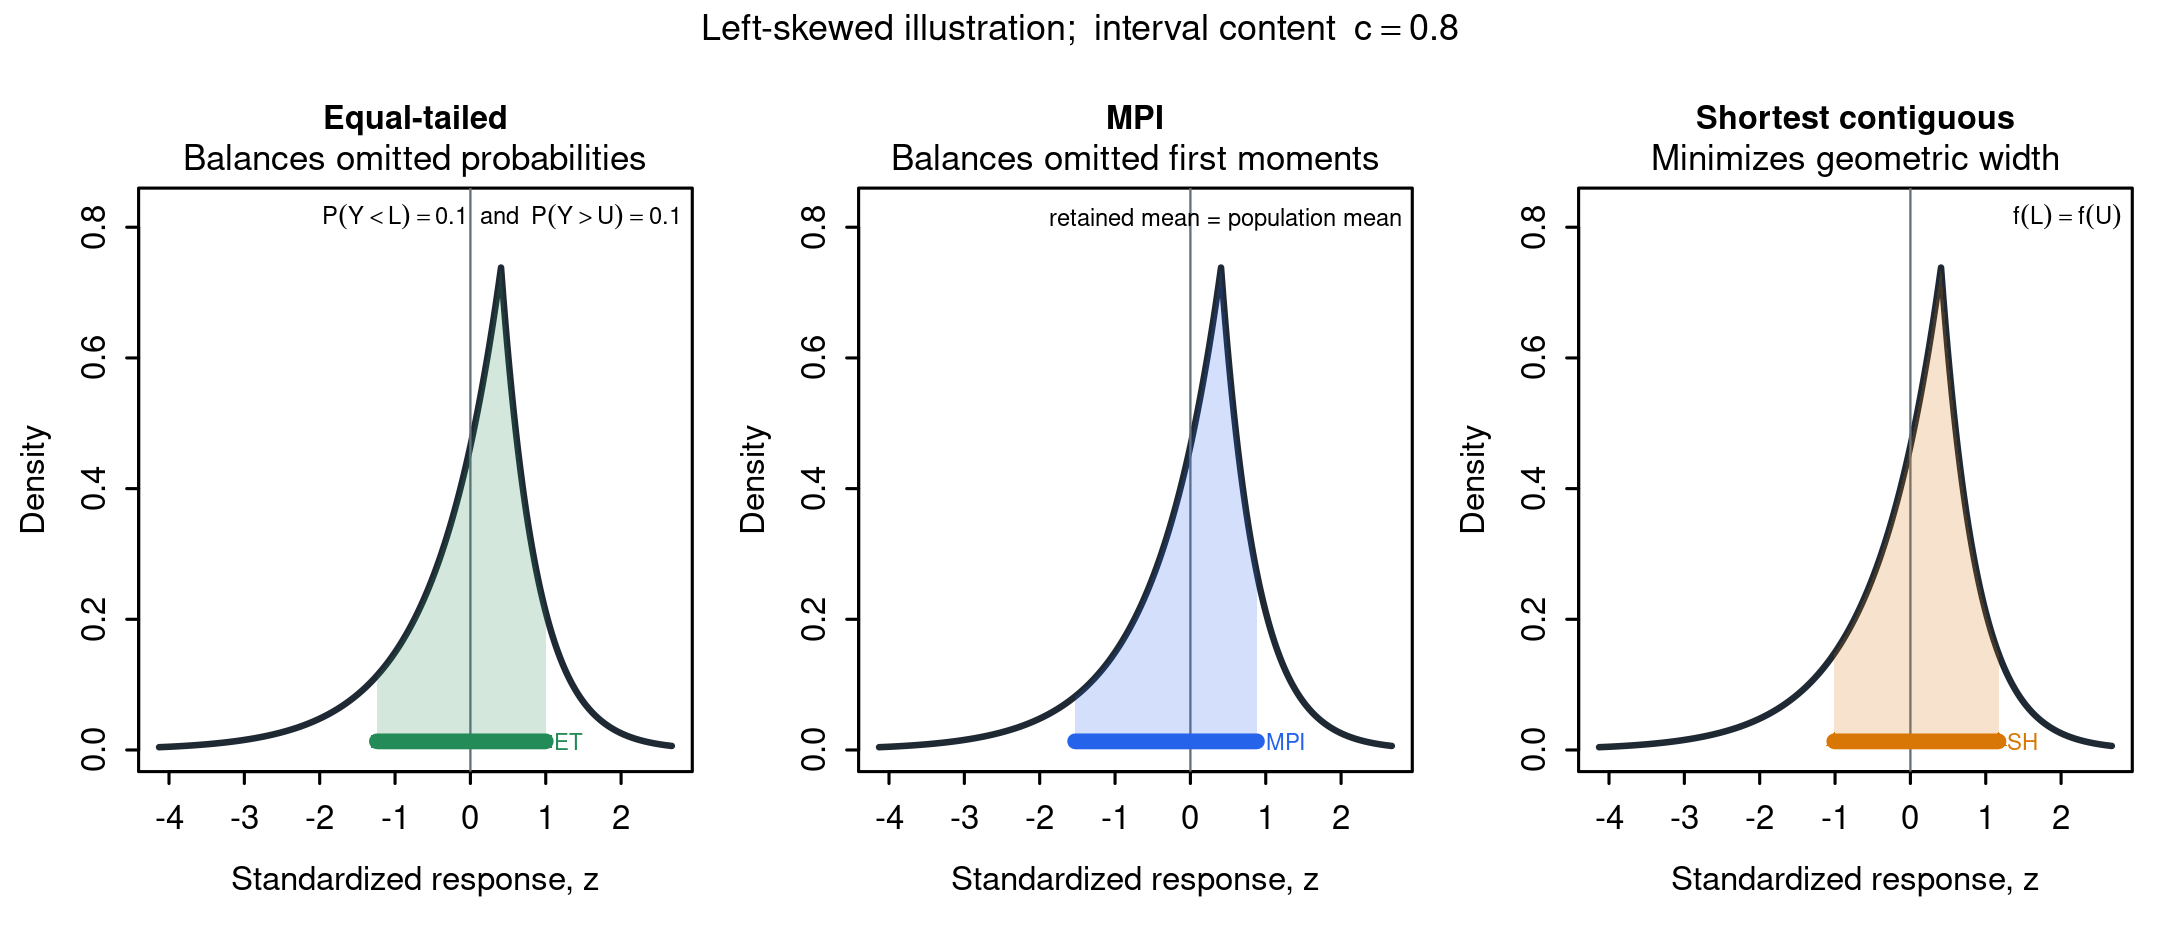
\includegraphics[width=\textwidth]{figures/ch05-mti/generated/fig01_three_balance_principles.png}
\caption{\textbf{Three interval-selection principles under left skewness.}
All panels use the same continuous left-skewed population illustration with
content \(c=0.80\), displayed after standardization. Equal-tailed (ET)
intervals balance omitted probabilities, MPI balances omitted first
moments, and shortest-contiguous (SH) intervals minimize geometric width.
These deterministic population calculations compare functionals; they are not
finite-sample or comparative-performance evidence.}
\label{rqr:fig:three-interval-principles}
\end{figure}

\section{Proofs for Fixed-Content Interval Targets}
\label{rqr:sec:supp-interval-functionals}

The population interval class is most transparent on the probability scale.
Suppress \(x\) and write
\[
I_c(u)=[Q(u),Q(u+c)],\qquad
M_c(u)=\frac{1}{c}\int_u^{u+c}Q(v)\,dv,\qquad
W_c(u)=Q(u+c)-Q(u).
\]
The equal-tailed interval fixes \(u_{\mathrm{ET}}=(1-c)/2\). MPI
solves \(M_c(u_{\mathrm{MPI}})=\mu\). Define the possibly set-valued collection
of shortest contiguous windows by
\[
S_{\mathrm{SH}}
=\argmin_{0\le u\le1-c}W_c(u).
\]
If a positive density exists at an interior \(u_{\mathrm{SH}}\in
S_{\mathrm{SH}}\), then
\[
W_c'(u_{\mathrm{SH}})
=\frac{1}{f\{Q(u_{\mathrm{SH}}+c)\}}
-\frac{1}{f\{Q(u_{\mathrm{SH}})\}}=0,
\]
so the endpoint densities agree. For a continuous strictly unimodal density
and a unique regular shortest interval, this interval agrees with the
corresponding highest-density interval. Under multimodality, a highest-density
region can be disconnected; the present construction remains restricted to
one contiguous interval
\citep{rqr-BrehmerGneiting2021Intervals}.

Under a symmetric unimodal distribution, all three intervals coincide. Under
asymmetry, their widths need not coincide; only the shortest interval is
ordered against the other two by definition. The standard interval score is
aligned with the central equal-tailed target and is not a target-neutral score
for this comparison
\citep{exd-gneiting2007,rqr-BrehmerGneiting2021Intervals,rqr-FisslerEtAl2021SetValued}.

\section{The Mean-Preserving Interval Target}
\label{rqr:sec:mpi-loss}

The residual-product loss becomes a statistical procedure once its target is
identified. This section first defines the pointwise loss, then shows that its
regular unrestricted population solution is the mean-preserving member of the
fixed-content interval class.

Fix a desired interval content \(c\in(0,1)\) and ordered endpoints \(a<b\).
The pointwise MPI loss is
\begin{equation}
\ell_c^{\mathrm{MPI}}(a,b;y)=
\begin{cases}
(1-c)(y-a)(b-y), & a<y<b,\\
c(y-a)(y-b), & y\le a\ \text{or}\ y\ge b.
\end{cases}
\label{rqr:eq:mpi-loss-piecewise}
\end{equation}
Both branches are nonnegative and meet continuously at zero when \(y=a\) or
\(y=b\). An observation inside the interval is weighted by \(1-c\), whereas a
miss is weighted by \(c\). The two factors also encode distance from both
endpoints, so the criterion weights membership and endpoint displacement
together. Increasing \(c\) raises the relative cost of a miss; at a regular
population optimum, this weighting
produces the content equation established below. For data
\(y_1,\ldots,y_n\), MPI minimizes
\(\sum_{i=1}^n\ell_c^{\mathrm{MPI}}(a,b;y_i)\), or the corresponding regression
loss when the two endpoints depend on predictors.

The familiar check-loss notation gives an equivalent compact representation.
For a scalar argument \(r\), let
\[
\rho_c(r)=r\{c-\ind(r<0)\}
=
\begin{cases}
(1-c)|r|, & r<0,\\
cr, & r\ge0.
\end{cases}
\]
Now define the product residual
\[
e(a,b;y)=(y-a)(y-b).
\]
Because \(e(a,b;y)<0\) exactly when \(a<y<b\),
\begin{equation}
\ell_c^{\mathrm{MPI}}(a,b;y)=\rho_c\{e(a,b;y)\}.
\label{rqr:eq:mpi-product-check}
\end{equation}
This representation also makes clear that the loss is symmetric in its two
roots; the ordering \(a<b\) is imposed only to interpret them as lower and
upper endpoints.
The check loss therefore acts on the scalar product residual, not on
\(y-a\) or \(y-b\) separately. In particular, \(c\) is the desired interval
content; it is neither an assigned response-quantile level for either endpoint
nor the generalized-Bayes learning rate.

The midpoint--half-width parameterization makes the interval geometry
explicit. Write \(a=m-h\) and \(b=m+h\), where \(h>0\). Then
\[
e(a,b;Y)=(Y-m)^2-h^2,
\]
so \(e<0\) means that \(Y\) is within distance \(h\) of \(m\). The half-width
and midpoint are estimated jointly by minimizing the expected loss
\(R_c(a,b)=\E\{\ell_c^{\mathrm{MPI}}(a,b;Y)\}\). Its first-order conditions determine both
the interval content and its placement. The loss defines this population
estimand. When a generalized-Bayes update is used later for a fixed target, its
learning rate controls the strength of the loss update rather than the
population content. The results below concern an unrestricted pointwise
population problem. Restricted regression classes generally recover only
design-weighted projections of these identities.

The endpoint scores have two population consequences: they set the interval
content and make the retained conditional distribution preserve the conditional
mean.

\begin{proposition}[Mean-preserving score characterization]
\label{rqr:prop:population-characterization}
Fix \(x\) and let \(a<b\). Suppose
\(\E(Y^2\mid X=x)<\infty\), the conditional distribution has no mass at \(a\)
or \(b\), differentiation may be interchanged with conditional expectation,
and \((a,b)\) is an interior stationary point over an unrestricted pointwise
endpoint class. Then the two population first-order conditions imply
\[
\Pr(a<Y<b\mid X=x)=c,
\]
and
\[
\E\{Y\ind(a<Y<b)\mid X=x\}
=c\,\E(Y\mid X=x).
\]
Equivalently,
\[
\E(Y\mid a<Y<b,X=x)=\E(Y\mid X=x).
\]
\end{proposition}

The population content equation is due to
\citet{rqr-PouplinEtAl2024RQR}. The retained-mean equation is a further
consequence of the same first-order system: conditional on \(X=x\), interval
membership has zero covariance with \(Y\). In omitted-tail form, the same
identity balances first-moment mass around the conditional mean:
\[
\E[\{\mu_x-Y\}\ind(Y<a)\mid X=x]
=
\E[\{Y-\mu_x\}\ind(Y>b)\mid X=x],
\qquad \mu_x=\E(Y\mid X=x).
\]
Tail probabilities may differ; MPI balances their first moments around
\(\mu_x\). The retained core and its excluded complement consequently have the
same conditional mean, although the endpoint midpoint may differ from that
mean. The integrated material further shows that the retained core is a mean-preserving
contraction of the full distribution in convex order. A finite first moment is
enough for the retained-mean identity once the endpoint scores are valid. The
stronger second-moment assumption ensures that the expected MPI loss
is finite and supports the profiled-risk analysis. This distinction matters
because the loss grows quadratically in an extreme response.

The next theorem converts the score identities into a quantile-window
functional. This is the object that the unrestricted population loss estimates.

\begin{theorem}[Quantile-window identification]
\label{rqr:thm:quantile-window}
In addition to the conditions of
Proposition~\ref{rqr:prop:population-characterization}, suppose that \(F_x\) is
continuous and strictly increasing on its support, and let \(Q_x=F_x^{-1}\).
Define
\[
M_{c,x}(u)=\frac{1}{c}\int_u^{u+c}Q_x(v)\,dv,
\qquad 0\le u\le1-c.
\]
Then \(M_{c,x}\) is strictly increasing. There is a unique index \(u_c(x)\)
satisfying
\[
M_{c,x}\{u_c(x)\}=\mu_x.
\]
The nondegenerate unrestricted MPI stationary interval is therefore
\[
a_c(x)=Q_x\{u_c(x)\},\qquad
b_c(x)=Q_x\{u_c(x)+c\}.
\]
If \(F_x\) is symmetric about \(\mu_x\), then
\(u_c(x)=(1-c)/2\), and the MPI and equal-tailed intervals coincide.
\end{theorem}

This theorem identifies the unique regular stationary window.
Theorem~\ref{rqr:thm:profiled-mean-tilt} below strengthens that statement to
the unique global expected-loss minimizer by profiling over the half-width.
The integrated material proves these results and records the restricted score
equations. Under the connected-support and local positive-density conditions
used in Theorem~\ref{rqr:thm:profiled-mean-tilt}, the regular unrestricted
population intervals form a nested path. If the conditional quantile function
is continuous at \(p_{\mu,x}=F_x(\mu_x)\) and
\(Q_x(p_{\mu,x})=\mu_x\), the two endpoints converge to \(\mu_x\) as
\(c\downarrow0\). Without this local support condition, the zero-content
limit may straddle a support gap. At fixed positive content, the midpoint's
role remains interval placement, while the conditional mean is imposed through
retained-mean balance. If the
conditional law has endpoint atoms,
the corresponding directional conditions give
\[
\Pr(a<Y<b\mid X=x)\le c\le\Pr(a\le Y\le b\mid X=x),
\]
so exact open-interval coverage requires endpoint continuity. Coincident roots
reduce the loss to \(c(Y-a)^2\) and target the conditional mean rather than a
nontrivial interval. Exact retained-mean equality is not asserted at endpoint
atoms without a separate joint subgradient and mass-allocation analysis.

MPI therefore targets an interval directly and can accommodate asymmetric
conditional distributions without assigning endpoint quantile levels in
advance. The characterization is pointwise and unrestricted; it holds only
under the stated conditions. Linear and other restricted root classes instead
satisfy design-weighted score equations and need not attain conditional
coverage or mean preservation at every covariate value. Nor does the
finite-sample unbiasedness argument for fixed endpoints apply automatically to
fitted endpoints: the endpoints depend on the data, and the empirical
objective is nonsmooth when an observation coincides with a root. Finite-sample
or asymptotic guarantees require a separate empirical-process argument.

\section{Mean-Preserving Interval Scores}
\label{rqr:sec:supp-population-target}

The derivation starts from the endpoint scores because those scores determine
both content and placement. Fix a covariate value \(x\), a desired content
\(c\in(0,1)\), and endpoints
\(a=L(x)<U(x)=b\). The pointwise loss is
\begin{equation}
\ell_c(a,b;y)
=
\begin{cases}
(1-c)(y-a)(b-y), & a<y<b,\\
c(y-a)(y-b), & y\le a\ \text{or}\ y\ge b.
\end{cases}
\label{rqr:eq:supp-mpi-loss-piecewise}
\end{equation}
Equivalently, with
\(e(a,b;y)=(y-a)(y-b)\) and
\(\rho_c(r)=r\{c-\ind(r<0)\}\),
\begin{equation}
\ell_c(a,b;y)=\rho_c\{e(a,b;y)\}.
\label{rqr:eq:supp-mpi-product-check}
\end{equation}
The check function is applied to the product residual. Its index \(c\) denotes
the desired interval content rather than a prescribed response-quantile level
for either endpoint or a generalized-Bayes learning rate. The loss is symmetric
in its two roots; ordering is used only for the endpoint interpretation.

Define \(I_{a,b}(Y)=\ind(a<Y<b)\). Away from the two roots, the derivative of
the check loss with respect to its scalar argument is
\(c-I_{a,b}(Y)\). Assume
\(\E(Y^2\mid X=x)<\infty\), the conditional risk is differentiable at an
interior stationary point, differentiation and conditional expectation may be
interchanged, and the conditional distribution places no mass at \(a\) or
\(b\). Since
\[
\frac{\partial}{\partial a}(Y-a)(Y-b)=b-Y,
\qquad
\frac{\partial}{\partial b}(Y-a)(Y-b)=a-Y,
\]
the pointwise first-order conditions are
\begin{align}
\E\left[\{c-I_{a,b}(Y)\}(b-Y)\mid X=x\right]&=0,
\label{rqr:eq:pop-foc-a}\\
\E\left[\{c-I_{a,b}(Y)\}(a-Y)\mid X=x\right]&=0.
\label{rqr:eq:pop-foc-b}
\end{align}
Subtracting \eqref{rqr:eq:pop-foc-b} from \eqref{rqr:eq:pop-foc-a} and using
\(b-a>0\) gives
\[
\Pr\{a<Y<b\mid X=x\}=c.
\]
Substitution into either first-order condition then gives
\[
\E\{Y\ind(a<Y<b)\mid X=x\}=c\E(Y\mid X=x).
\]

The second equation is equivalently
\[
\E(Y\mid a<Y<b,X=x)=\E(Y\mid X=x)
\]
and
\(\operatorname{Cov}\{Y,I_{a,b}(Y)\mid X=x\}=0\). This covariance statement is
compatible with dependence, asymmetry, and unequal-tailed endpoints. The
coverage implication is established by \citet{rqr-PouplinEtAl2024RQR}; the
conditional first-moment implication is a further consequence of their
first-order system.

Let \(\mu_x=\E(Y\mid X=x)\). Since
\(\E(Y-\mu_x\mid X=x)=0\), the first-moment equation is also equivalent to
\begin{equation}
\E[\{\mu_x-Y\}\ind(Y<a)\mid X=x]
=
\E[\{Y-\mu_x\}\ind(Y>b)\mid X=x].
\label{rqr:eq:rqr-tail-moment-balance}
\end{equation}
Thus MPI balances omitted tail probability multiplied by average
tail displacement from the conditional mean. The two omitted tail probabilities
may differ.

\begin{theorem}[Quantile-window identification]
\label{rqr:thm:supp-quantile-window}
Suppose, in addition, that \(F_x\) is continuous and strictly increasing on
its support, and let \(Q_x=F_x^{-1}\). Define
\[
M_{c,x}(u)=\frac{1}{c}\int_u^{u+c}Q_x(v)\,dv,
\qquad 0\le u\le1-c.
\]
Then \(M_{c,x}\) is strictly increasing, and there is a unique \(u_c(x)\)
satisfying \(M_{c,x}\{u_c(x)\}=\mu_x\). The corresponding interval is
\[
\left[Q_x\{u_c(x)\},Q_x\{u_c(x)+c\}\right].
\]
\end{theorem}

\begin{proof}
Modulo conditional probability-zero portions outside the support, every
contiguous interval having content \(c\) has the displayed
quantile-window form. If \(v>u\), then
\[
M_{c,x}(v)-M_{c,x}(u)
=\frac{1}{c}\int_0^c
\{Q_x(v+s)-Q_x(u+s)\}\,ds>0.
\]
The average of the lowest conditional \(c\)-fraction is below \(\mu_x\), and
the average of the highest conditional \(c\)-fraction is above \(\mu_x\), for
a nondegenerate distribution with finite mean. Continuity and strict
monotonicity therefore give existence and uniqueness. The first-moment
equation identifies the stated endpoints.
\end{proof}

If \(F_x\) is symmetric about \(\mu_x\), then
\(Q_x(1-v)=2\mu_x-Q_x(v)\). The window beginning at
\((1-c)/2\) has retained mean \(\mu_x\), so uniqueness gives the equal-tailed
interval. Conversely, coincidence at one coverage level does not establish
global symmetry.

The distribution conditional on interval membership and its complementary
tail distribution both have mean \(\mu_x\). This is a first-moment statement,
not independence between \(Y\) and interval membership. It also clarifies why
the endpoint midpoint need not equal \(\mu_x\) under asymmetry.

\begin{proposition}[Mean-preserving contraction]
\label{rqr:prop:supp-convex-order}
Let \(Y_{\mathrm{in}}\) and \(Y_{\mathrm{out}}\) have the conditional
distributions of \(Y\) given \(a<Y<b\) and \(Y\notin(a,b)\), respectively,
at a regular MPI target. For every convex function \(\varphi\) for
which the required expectations exist,
\[
\E\{\varphi(Y_{\mathrm{in}})\}
\le
\E\{\varphi(Y)\}
\le
\E\{\varphi(Y_{\mathrm{out}})\}.
\]
Consequently,
\[
Y_{\mathrm{in}}\preceq_{\mathrm{cx}}Y
\preceq_{\mathrm{cx}}Y_{\mathrm{out}}.
\]
If second moments exist, the same ordering holds for the corresponding
variances.
\end{proposition}

\begin{proof}
Let \(s_\varphi\) be the affine secant through
\(\{a,\varphi(a)\}\) and \(\{b,\varphi(b)\}\). Convexity gives
\(\varphi(y)\le s_\varphi(y)\) on \([a,b]\) and
\(\varphi(y)\ge s_\varphi(y)\) outside that interval. Both conditional
distributions have mean \(\mu_x\), so
\[
\E\{\varphi(Y_{\mathrm{in}})\}
\le s_\varphi(\mu_x)
\le \E\{\varphi(Y_{\mathrm{out}})\}.
\]
The full conditional distribution is their mixture with weights \(c\) and
\(1-c\), which places its convex expectation between the two. Taking
\(\varphi(y)=(y-\mu_x)^2\) gives the variance statement.
\end{proof}

\subsection{Interval Paths and Tail Sensitivity}

Retain the quantile-window characterization and assume, for this derivative
calculation, connected support and positive continuous density at the relevant
endpoint quantiles. Write \(u_c\) for the MPI index, and set
\(L_c=Q(u_c)\) and \(U_c=Q(u_c+c)\). Differentiating
\[
\int_{u_c}^{u_c+c}\{Q(v)-\mu\}\,dv=0
\]
with respect to \(c\), at regular interior values, gives
\[
\frac{du_c}{dc}
=-\frac{U_c-\mu}{U_c-L_c}<0,
\qquad
\frac{d(u_c+c)}{dc}
=\frac{\mu-L_c}{U_c-L_c}>0.
\]
The MPI population intervals are therefore nested as content
increases, with analogous one-sided statements at isolated nonsmooth support
transitions. If \(p_\mu=F(\mu)\) satisfies \(Q(p_\mu)=\mu\) and \(Q\) is
continuous at \(p_\mu\), then \(Q(u_c)\le\mu\le Q(u_c+c)\), so
\(p_\mu\in[u_c,u_c+c]\). Since this probability window has length \(c\),
\[
L_c\longrightarrow\mu,\qquad U_c\longrightarrow\mu
\quad\text{as }c\downarrow0.
\]
This zero-content limit needs the local support condition above. It is false
under the quantile-window assumptions alone: for the symmetric distribution
with density \(1/2\) on \([-2,-1]\cup[1,2]\), \(\mu=0\) and the MPI
window has \(u_c=(1-c)/2\), hence \(L_c=-1-c\) and \(U_c=1+c\), so the
zero-content limit straddles the support gap rather than contracting to
\(\mu\). The corrected zero-content limit is a property of the population
interval path; the
midpoint at a fixed positive \(c\) is not generally the mean, and independent
fits at several content levels do not by themselves define joint
generalized-posterior draws of that path.

For \(Y^\star=r+sY\), \(s>0\), the MPI endpoints transform as
\[
L_c^\star=r+sL_c,\qquad U_c^\star=r+sU_c.
\]
For the tilted family, \(\delta^\star=s\delta\) and
\[
\ell^\star_{c,\delta^\star}
(r+sa,r+sb;r+sy)
=s^2\ell_{c,\delta}(a,b;y).
\]
Thus the population target is positive-affine equivariant. A corresponding
generalized posterior uses the transformed prior and
\(\omega_{\mathrm R}^\star=\omega_{\mathrm R}/s^2\). Conversely, if the
original response is standardized as \(\widetilde Y=(Y-r)/s\), use
\(\widetilde\delta=\delta/s\) and
\(\widetilde\omega_{\mathrm R}=\omega_{\mathrm R}s^2\).
Nonlinear monotone transformations generally change the mean-preserving
functional rather than merely re-expressing it.

Finally, with fixed endpoints,
\(\rho_c\{(y-a)(y-b)\}=O(y^2)\) as \(|y|\to\infty\), and the endpoint scores
grow linearly in \(|y|\). MPI is distribution-free in the sense that it does
not posit a parametric response density. Its retained-mean target still depends
on second moments, so the finite-second-moment assumption and response-scale
choice are scientifically consequential.

Endpoint atoms require directional conditions. Write
\(m=(a+b)/2\), \(h=(b-a)/2>0\), so
\(e=(Y-m)^2-h^2\). The left and right derivatives in \(h\) are
\[
D_-R_x(m,h)=2h\{\Pr(a<Y<b\mid x)-c\},
\]
and
\[
D_+R_x(m,h)=2h\{\Pr(a\le Y\le b\mid x)-c\}.
\]
At a local minimum, \(D_-R_x\le0\le D_+R_x\), and therefore
\[
\Pr(a<Y<b\mid X=x)\le c\le\Pr(a\le Y\le b\mid X=x).
\]
Without a separate joint subgradient and endpoint-mass allocation analysis,
these directional conditions do not imply the exact retained-mean equality
derived above under endpoint continuity.
If \(a=b=m\), then \(e=(Y-m)^2\) and the risk is
\(c\E\{(Y-m)^2\mid X=x\}\); the coincident-root target is the conditional
mean when the second moment exists.

These implications are conditional, pointwise, and assumption dependent. They
do not follow by treating estimated data-dependent endpoints as fixed. For
linear roots \(\eta_k(X)=X^\top\beta_k\), the corresponding population score
conditions are instead
\begin{align}
\E\left[X\{c-I_{\eta_1,\eta_2}(Y)\}(\eta_2-Y)\right]&=0,\\
\E\left[X\{c-I_{\eta_1,\eta_2}(Y)\}(\eta_1-Y)\right]&=0,
\end{align}
where \(I_{\eta_1,\eta_2}(Y)\) indicates that \(Y\) lies between the
unordered roots. These design-weighted projection equations need not imply
conditional coverage for every \(x\).

The finite-sample unbiasedness calculation in
\citet{rqr-PouplinEtAl2024RQR} treats fitted, data-dependent endpoints as fixed,
and its zero-gradient argument does not cover nonsmooth optima when an
observation coincides with a fitted root. We therefore do not use that
calculation as a finite-sample guarantee; such a result requires a separate
empirical-process analysis.

\section{Mean-Tilted Intervals}
\label{rqr:sec:mti-loss}

The MTI family is the fixed-tilt generalization of MPI. It preserves the MPI
content score and replaces the zero retained-mean-balance equation by a fixed
retained-mean tilt \(\delta\), measured in response units. To move through the
content-\(c\) family without changing the coverage score, define
\[
\ell_{c,\delta}^{\mathrm{MTI}}(m,h;y)
=
\rho_c\{(y-m)^2-h^2\}-2c\delta(m-y).
\]
Equivalently,
\[
\ell_{c,\delta}^{\mathrm{MTI}}(a,b;y)
=
\rho_c\{(y-a)(y-b)\}-c\delta(a+b-2y).
\]
The second form shows that the loss remains invariant to exchanging the two
roots. MPI is exactly the \(\delta=0\) member of the MTI family.

This generalization changes placement but not content. The proposition records
that separation explicitly.

\begin{proposition}[Fixed-content mean tilt]
\label{rqr:prop:mean-tilt}
Under the regularity conditions of
Proposition~\ref{rqr:prop:population-characterization}, a nondegenerate interior
stationary point of the mean-tilted population risk satisfies
\[
\Pr(a_\delta<Y<b_\delta)=c,\qquad
\E(Y\mid a_\delta<Y<b_\delta)=\mu+\delta.
\]
If \(F\) is continuous and strictly increasing on its support, then for every
\(\delta\) strictly between \(M_c(0)-\mu\) and
\(M_c(1-c)-\mu\), its unique interior quantile-window index solves
\[
M_c(u_\delta)=\mu+\delta.
\]
\end{proposition}

The score equations identify stationary points. Global identification follows
by profiling over the unique content-\(c\) radius at each midpoint and
differentiating the profiled risk; the integrated technical material gives the radius and
envelope-derivative argument.

\begin{theorem}[Global identification of the MTI target]
\label{rqr:thm:profiled-mean-tilt}
Suppose that the support closure is an interval (possibly with infinite
endpoints), \(F\) is absolutely continuous and strictly increasing between its
support endpoints, its density is positive and continuous on the support
interior, and \(\E(Y^2)<\infty\). Extend \(F\) by zero and one beyond finite
support endpoints. For every tilt satisfying
\[
M_c(0)-\mu<\delta<M_c(1-c)-\mu,
\]
the expected MTI loss has a unique global minimizer over finite ordered
roots. Its probability-window index \(u_\delta\in(0,1-c)\) is the unique
solution of
\[
M_c(u_\delta)=\mu+\delta.
\]
Nondegeneracy gives \(M_c(0)<\mu<M_c(1-c)\), so MPI is the interior
special case \(\delta=0\).
\end{theorem}

Finite second moments make both endpoint tilt values finite, even when a
support endpoint is infinite. Boundary tilts correspond to one-sided
probability-window limits. Infinite support endpoints lead to semi-infinite
limiting intervals, and finite endpoints require a support constraint to choose
a unique inactive-root representation. Outside the closed admissible tilt range,
the unrestricted risk is unbounded below along the corresponding escaping-root
direction. A proper Gaussian prior can nevertheless yield a proper
finite-sample generalized posterior.

The recovery tilts translate familiar placement rules into the MTI coordinate.
There are three distinct uses of the tilt notation. A fixed target tilt is
chosen before generalized-posterior computation; a population recovery tilt
identifies which \(\delta\) reproduces a familiar interval functional under a
known distribution; an empirical plug-in tilt estimates such a value through a
separate target-selection rule.

\begin{corollary}[Recovery tilts for familiar interval functionals]
\label{rqr:cor:recovery-tilts}
MPI is recovered by \(\delta_{\mathrm{MPI}}=0\). Define
\[
S_{\mathrm{SH}}
=
\argmin_{0\le u\le1-c}W_c(u),\qquad
\Delta_{\mathrm{SH}}
=
\{M_c(u)-\mu:u\in S_{\mathrm{SH}}\}.
\]
The population recovery tilt for the equal-tailed interval is
\[
\delta_{\mathrm{ET}}=M_c\{(1-c)/2\}-\mu.
\]
Each \(u\in S_{\mathrm{SH}}\) has recovery tilt
\(\delta_{\mathrm{SH}}(u)=M_c(u)-\mu\). Singular notation is used only when the
shortest-contiguous window is unique or one minimizer has been selected.
\end{corollary}

At regular interior points where the endpoint quantiles are differentiable
and have positive densities,
\[
\frac{du_\delta}{d\delta}=\frac{c}{W_c(u_\delta)},\qquad
\frac{dW_c(u_\delta)}{d\delta}
=\frac{c\,W_c'(u_\delta)}{W_c(u_\delta)}.
\]
Thus an interior width minimum along the tilt path satisfies the usual
equal-endpoint-density condition.
Figure~\ref{rqr:fig:mean-tilt-map} visualizes the same recovery map across
symmetric and skewed population laws before adding any finite-sample
approximation layer.

\begin{figure}[!htbp]
\centering
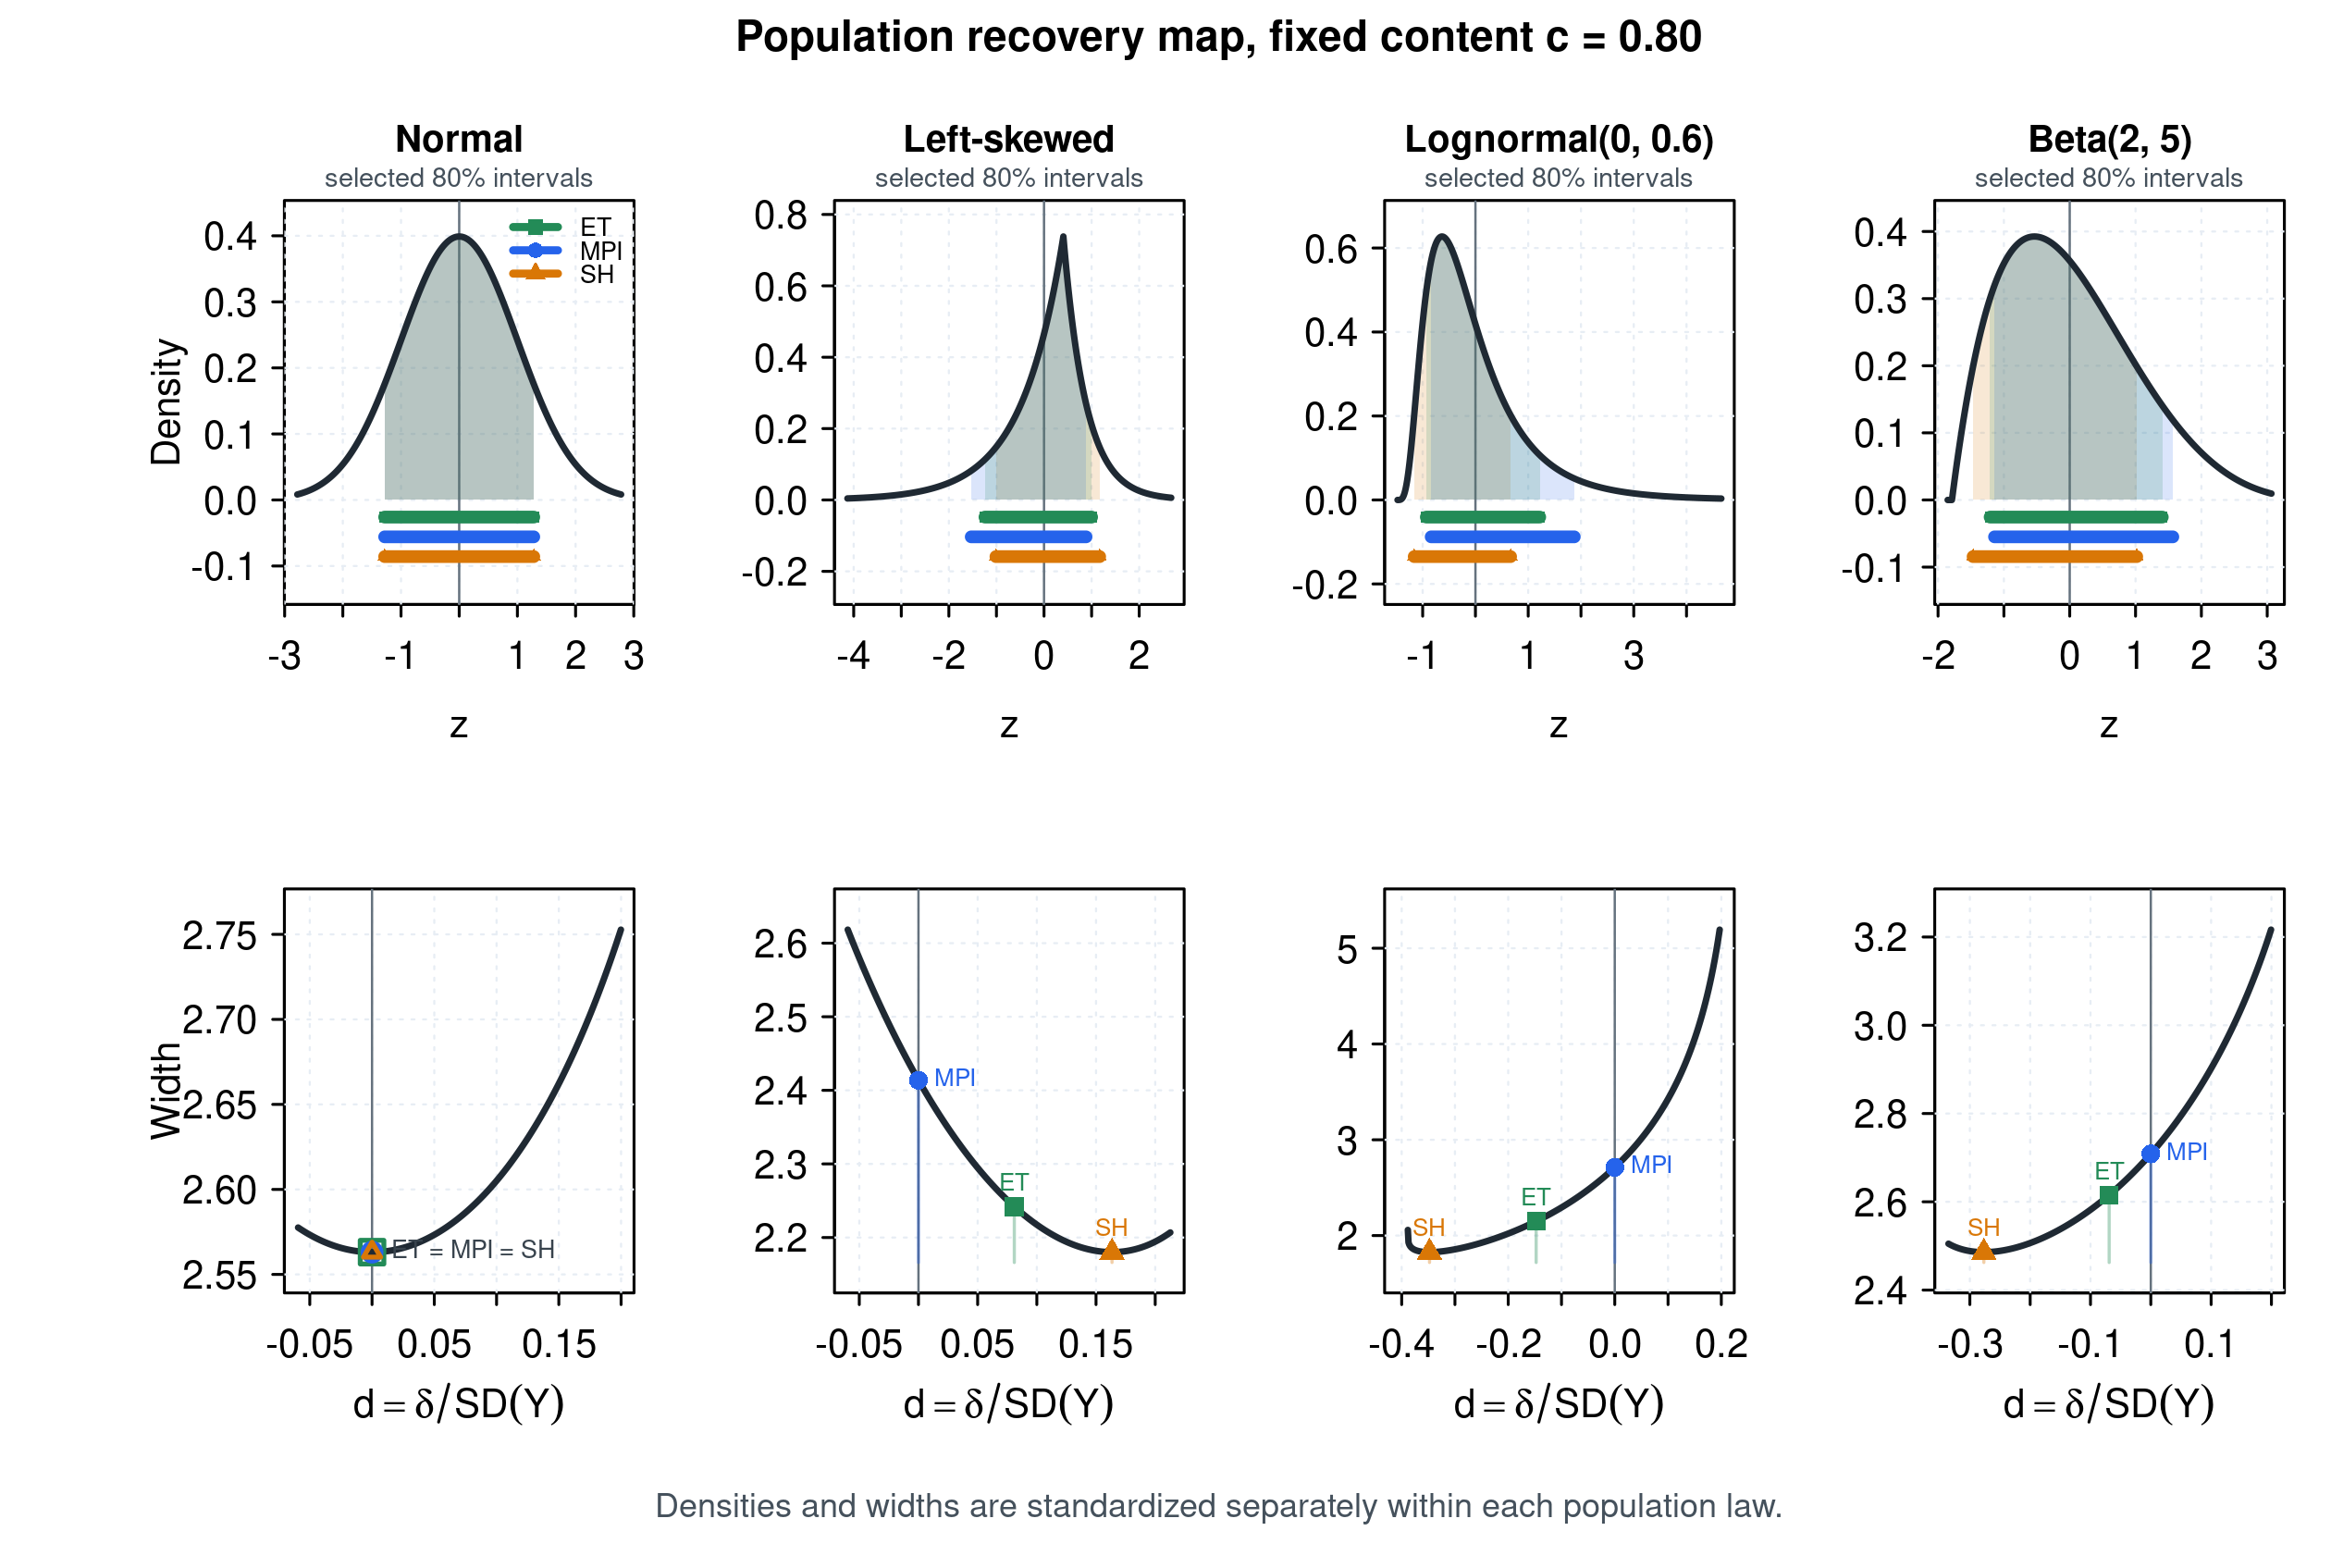
\includegraphics[width=\textwidth]{figures/ch05-mti/generated/figS01_cross_distribution_recovery.png}
\caption{\textbf{Population recovery tilts across symmetric and skewed
distributions.}
Every interval has content \(c=0.80\). Targets are computed on each raw
population law and then displayed after mean/standard-deviation
standardization. The top row shows standardized densities with equal-tailed
  (ET), MPI, and shortest-contiguous (SH) intervals; the bottom row
  shows the standardized width profile along the MTI family. In the
Normal reference case the three targets coincide at
\(\delta/\operatorname{SD}(Y)=0\). Under skewness, ET and SH generally require
  nonzero, distribution-specific recovery tilts, while MPI remains the
zero-tilt retained-mean-balance target. The deterministic display is a
population map for external target specification.}
\label{rqr:fig:mean-tilt-map}
\end{figure}

For initialization and external tilt selection, the same identities suggest a
simple first-order approximation. Let \(\gamma_1\) denote standardized
skewness and set
\[
q_c=\Phi^{-1}\{(1+c)/2\},\qquad K_c=q_c\phi(q_c)/c.
\]
A Cornish--Fisher expansion around a standardized Normal law
\citep{rqr-CornishFisher1937} gives the
shortest-oriented and equal-tailed standardized tilt approximations
\[
d_{\mathrm{SH}}^{\mathrm{CF}}=-\gamma_1K_c,\qquad
d_{\mathrm{ET}}^{\mathrm{CF}}=\frac{1}{3}d_{\mathrm{SH}}^{\mathrm{CF}},
\qquad d=\delta/\operatorname{SD}(Y).
\]
These formulas are not new interval targets; they are local skewness-based
approximations to the population recovery tilts. Right skewness gives a
negative shortest-oriented tilt, while left skewness gives a positive tilt.
They supply simple, interpretable starting values for tilt exploration, not
automatic shortest-interval estimators. Figure~\ref{rqr:fig:mean-tilt-cf-anchors}
places the two approximations on the exact population tilt path using true
population skewness rather than a sample estimate.

\begin{figure}[H]
\centering
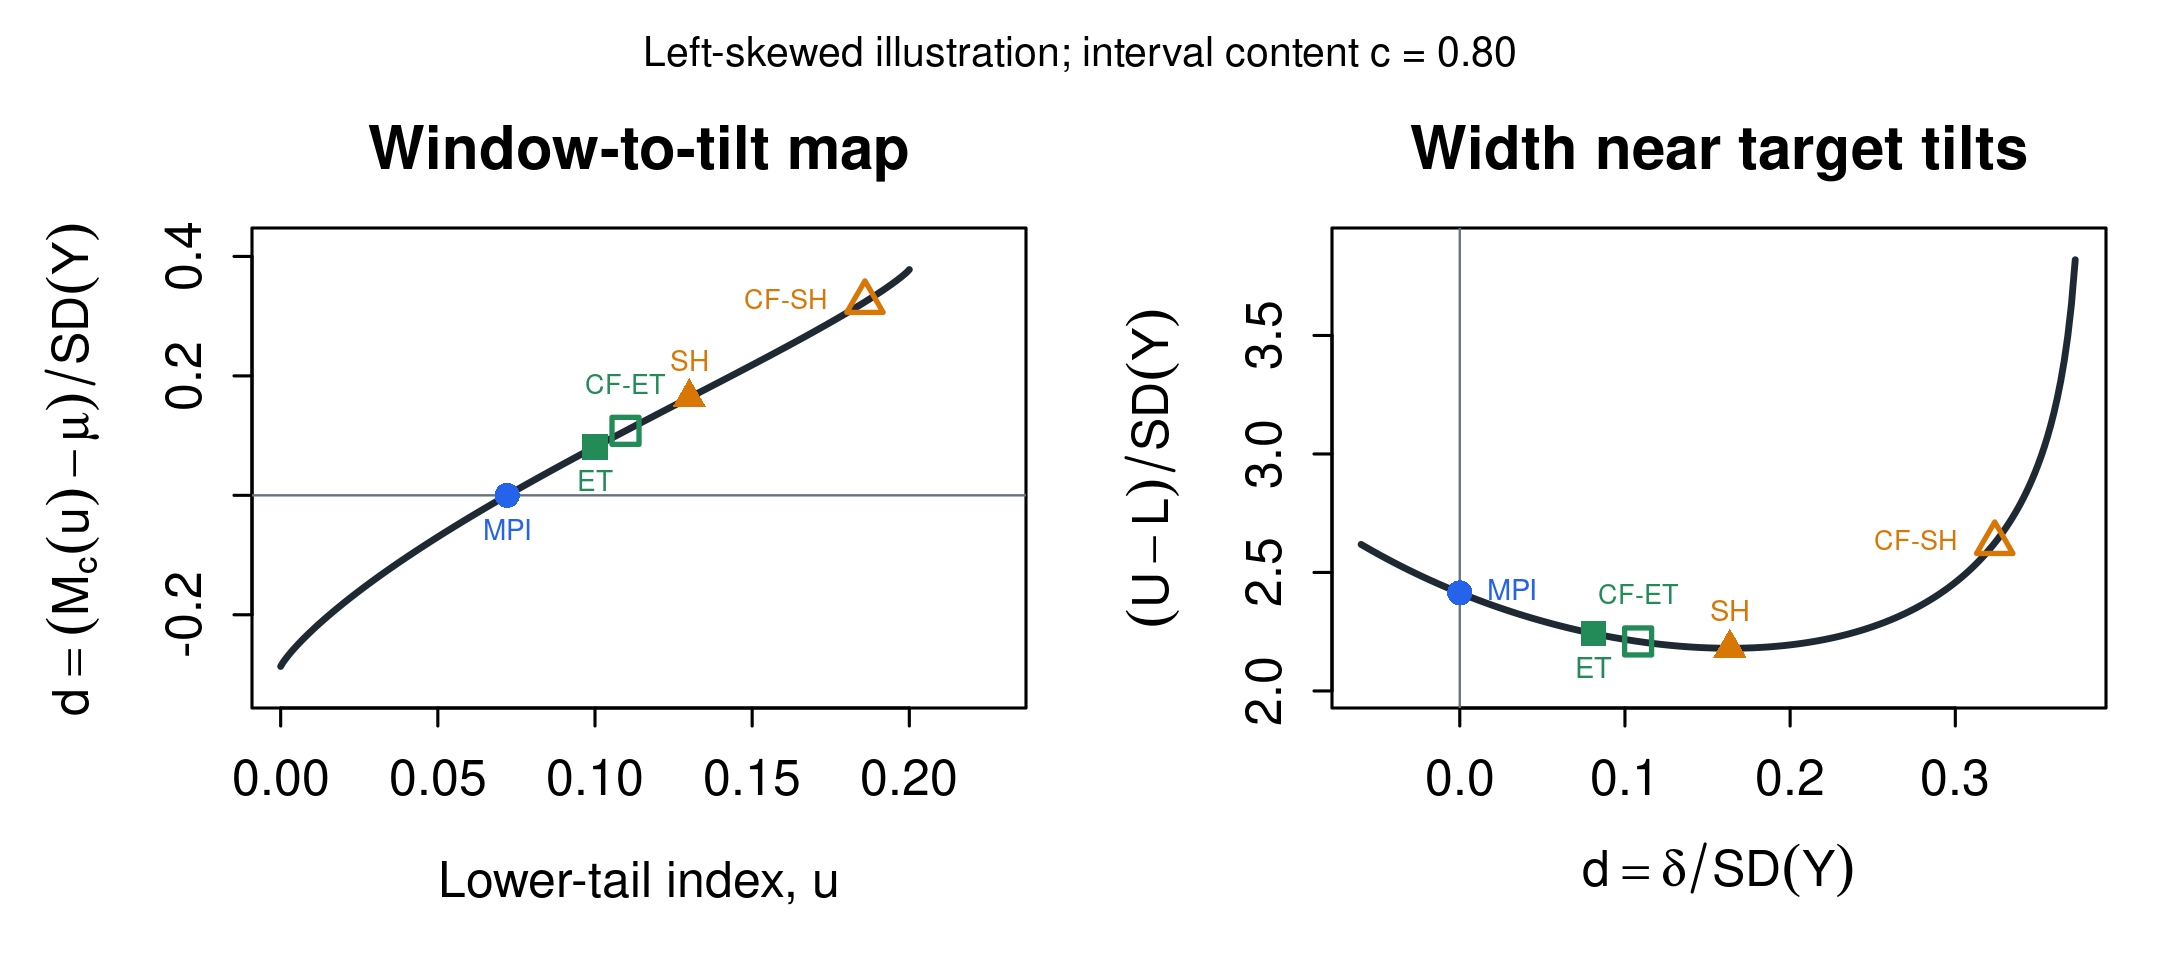
\includegraphics[width=\textwidth]{figures/ch05-mti/generated/fig03_mean_tilt_cf_anchors.png}
\caption{\textbf{Cornish--Fisher recovery-tilt approximation.}
For content \(c=0.80\), the solid curves are the population window-to-tilt
map and width profile from the left-skewed illustration. Filled markers are
the exact population MPI, ET, and SH tilts. Open markers are the first-order
Cornish--Fisher approximations computed from true population skewness. The display
diagnoses a population approximation for initialization and external
tilt selection. Data-driven tilt estimation, MCMC evidence, and response prediction
are separate empirical tasks.}
\label{rqr:fig:mean-tilt-cf-anchors}
\end{figure}

\begin{table}[H]
\centering
\caption{\textbf{Population accuracy of first-order Cornish--Fisher recovery-tilt approximations.} Each row uses a known population law, content $c=0.80$, and true skewness $\gamma_1$. Population and CF columns report standardized recovery tilts $d=\delta/\operatorname{SD}(Y)$; $|e|$ is their absolute gap. Gamma arguments are shape and scale, lognormal arguments are meanlog and sdlog, and the exponential law has unit rate. $^{\dagger}$ denotes an SH population value at the lower support boundary. This is a deterministic population calculation, not MCMC, tilt-selection, or response-prediction evidence.}
\label{rqr:tab:mean-tilt-cf-mini-study}
\TableStyle
\begin{tabular}{@{}l@{\hspace{0.8em}}rrrrrrr@{}}
\toprule
Distribution & $\gamma_1$ & \multicolumn{3}{c}{Equal-tailed} & \multicolumn{3}{c}{Shortest-contiguous} \\
\cmidrule(lr){3-5} \cmidrule(l){6-8}
& & Population $d$ & CF $d$ & $|e|$ & Population $d$ & CF $d$ & $|e|$ \\
\midrule
Normal & 0.000 & 0.000 & 0.000 & 0.000 & 0.000 & 0.000 & 0.000 \\
Gamma(16, 0.25) & 0.500 & -0.047 & -0.047 & 0.000 & -0.140 & -0.141 & 0.001 \\
Gamma(4, 1) & 1.000 & -0.092 & -0.094 & 0.002 & -0.273 & -0.281 & 0.008 \\
Lognormal(0, 0.5) & 1.750 & -0.128 & -0.164 & 0.036 & -0.323 & -0.492 & 0.169 \\
Exponential$^{\dagger}$ & 2.000 & -0.169 & -0.187 & 0.018 & -0.402 & -0.562 & 0.160 \\
Beta(2, 5) & 0.596 & -0.069 & -0.056 & 0.013 & -0.277 & -0.168 & 0.109 \\
Beta(5, 2) & -0.596 & 0.069 & 0.056 & 0.013 & 0.277 & 0.168 & 0.109 \\
\bottomrule
\end{tabular}
\end{table}


Table~\ref{rqr:tab:mean-tilt-cf-mini-study} shows why the approximation should
remain an approximation rather than a target definition. It is exact at symmetry and
close for the near-Normal Gamma laws. Its errors are larger for lognormal and
bounded Beta shapes and for the exponential law, whose shortest interval is a
support-boundary solution. The reflected Beta rows verify the expected sign
reversal but also show that skewness alone does not determine approximation
accuracy. Across these examples the ET approximation is more accurate than the
SH approximation, but that comparison is descriptive rather than a general
ordering.
The numerical summaries therefore report moment shape,
probability-window boundary behavior, and bootstrap sensitivity whenever a
sample plug-in approximation is constructed.

The recovery tilts above are population quantities. A universal tilt does not
recover the same interval functional across distributions, and conditional
recovery generally requires a covariate-dependent \(\delta(x)\). The tilt is
therefore fixed or selected by a separate validation rule; sampling
it as an ordinary parameter would mix distinct interval targets. The target is
equivariant under positive affine changes of response scale when \(\delta\)
and the fixed learning rate are transformed accordingly, but it is not
invariant to arbitrary monotone response transformations. Generalized-Bayes
computations with nonzero tilt require the target content, tilt, learning rate,
and prior class to be specified before the loss update is evaluated. Other
prior, learning-rate, and model classes require separate propriety arguments and
validation. Data-driven tilt selection likewise requires an independent
selection rule before empirical claims are made.

The population score equations do not by themselves establish propriety of a
finite-sample generalized posterior under an arbitrary root prior. With a
fixed learning rate, a finite design, and proper Gaussian root priors, the tilt
is linear in the root parameters and the Gaussian tails make the generalized
posterior proper. This argument covers ridge regression with proper Gaussian
root priors. Heavier-tailed shrinkage priors and dependent root processes
require separate propriety analyses before nonzero tilt is considered.

\section{Mean-Tilted Interval Loss and Target}
\label{rqr:sec:supp-mean-tilt}

The MTI loss is the fixed-tilt generalization of MPI. It keeps the MPI content
score and shifts only the retained-mean equation; setting \(\delta=0\) recovers
the MPI loss. For a fixed mean tilt \(\delta\in\R\), define
\begin{equation}
\ell_{c,\delta}^{\mathrm{MTI}}(m,h;y)
=\rho_c\{(y-m)^2-h^2\}-2c\delta(m-y),
\label{rqr:eq:mean-tilted-loss-midpoint}
\end{equation}
or, equivalently,
\begin{equation}
\ell_{c,\delta}^{\mathrm{MTI}}(a,b;y)
=\rho_c\{(y-a)(y-b)\}-c\delta(a+b-2y).
\label{rqr:eq:mean-tilted-loss-roots}
\end{equation}
The second form is invariant to exchanging the raw root labels. The tilt has
response units so that both terms in the loss have squared-response units, and
nonzero \(\delta\) changes the target placement rather than the content score.
For restricted linear roots \(\eta_k(X)=X^\top\beta_k\) and an externally
fixed \(\delta(X)\), the population score equations are
\begin{align}
\E\!\left[
X\left\{\{c-I_{\eta_1,\eta_2}(Y)\}(\eta_2-Y)-c\delta(X)\right\}
\right]&=0,\\
\E\!\left[
X\left\{\{c-I_{\eta_1,\eta_2}(Y)\}(\eta_1-Y)-c\delta(X)\right\}
\right]&=0.
\end{align}
They are design-weighted projection equations. Pointwise conditional content
and retained-mean identities require a sufficiently rich predictor class and
the unrestricted conditions below.

\subsection{Fixed-Content Mean-Tilted Target}

The next proposition records the population score equations supported by the
mean-tilted loss. It is the integrated counterpart of
the fixed-content mean-tilt proposition in the main article.

\begin{proposition}[Fixed-content mean-tilted target]
\label{rqr:prop:supp-mean-tilt}
Under the regularity conditions in
Section~\ref{rqr:sec:supp-population-target}, a nondegenerate interior
stationary point \((m_\delta,h_\delta)\) satisfies
\[
\Pr(|Y-m_\delta|<h_\delta)=c
\]
and
\[
\E(Y\mid |Y-m_\delta|<h_\delta)=\mu+\delta.
\]
If \(F\) is continuous and strictly increasing on its support and \(\delta\)
lies strictly between the endpoint values of the admissible range, the unique
interior lower-tail index is the solution of
\[
M_c(u_\delta)=\mu+\delta.
\]
Endpoint tilts are understood as boundary limits and satisfy the corresponding
one-sided stationarity conditions.
\end{proposition}

\begin{proof}
Let \(I_{m,h}(Y)=\ind(|Y-m|<h)\). Away from endpoint atoms,
\begin{align}
\frac{\partial}{\partial h}\E\{\ell_{c,\delta}(m,h;Y)\}
&=2h\{\Pr(I_{m,h}=1)-c\},\\
\frac{\partial}{\partial m}\E\{\ell_{c,\delta}(m,h;Y)\}
&=2\E[(m-Y)\{c-I_{m,h}(Y)\}]-2c\delta.
\end{align}
The first equation gives content \(c\). Substitution into the second gives
\(\E\{YI_{m,h}(Y)\}=c(\mu+\delta)\), which is the retained-mean equation.
Theorem~\ref{rqr:thm:supp-quantile-window} and strict monotonicity of \(M_c\)
give the quantile-window statement.
\end{proof}

\begin{lemma}[Profile radius and envelope derivative]
\label{rqr:lem:supp-profile-radius}
Suppose that the support closure of \(F\) is an interval
\([\ell,r]\), where either endpoint may be infinite, \(F\) is continuous and
strictly increasing and absolutely continuous between its support endpoints,
its density is positive and continuous on the support interior, and
\(\E(Y^2)<\infty\). Extend \(F\) by zero and one beyond finite support
endpoints. For every \(m\in\R\), there is a unique \(h_c(m)>0\) satisfying
\[
\Pr\{|Y-m|<h_c(m)\}=c.
\]
The map \(m\mapsto h_c(m)\) is continuous and is differentiable whenever its
two roots are interior to the support. Define
\[
\overline R_{c,\delta}(m)
=
\E\{\ell_{c,\delta}(m,h_c(m);Y)\}.
\]
Also let \(u_c(m)=F\{m-h_c(m)\}\). Then
\begin{equation}
\overline R_{c,\delta}'(m)
=2c\left[M_c\{u_c(m)\}-\mu-\delta\right],
\label{rqr:eq:supp-profiled-risk-derivative}
\end{equation}
where both roots are interior, with the corresponding one-sided derivatives
when a root crosses a finite support endpoint.
\end{lemma}

\begin{proof}
For fixed \(m\), the map
\[
H_m(h)=F(m+h)-F(m-h),\qquad h\ge0,
\]
is continuous, begins at zero, and converges to one. Interval support and
strict increase imply that \(H_m\) passes through every value in \((0,1)\)
strictly: any plateau can occur only before the expanding interval reaches
the support or after it contains the full support. Thus \(H_m(h)=c\) has one
solution. Continuity of this inverse in \(m\) follows by the same strict
crossing argument. When both roots are interior, the implicit-function
theorem applies because
\[
\frac{\partial H_m(h)}{\partial h}
=f(m+h)+f(m-h)>0.
\]

For fixed \(m\), write \(Z_m=(Y-m)^2\) and \(q=h^2\). The subgradient interval
of \(q\mapsto\E\{\rho_c(Z_m-q)\}\) is
\[
\left[\Pr(Z_m<q)-c,\ \Pr(Z_m\le q)-c\right].
\]
Continuity makes \(q=h_c(m)^2\) its unique minimizer. On a compact
neighborhood of \(m\), the partial midpoint score is dominated by a constant
multiple of \(1+|Y|\), which is integrable. Differentiation under the
expectation is therefore valid away from the probability-zero endpoints.
The standard two-sided profiling inequalities, evaluated once at
\(h_c(m)\) and once at \(h_c(m+s)\), together with continuity of \(h_c\),
give the envelope derivative
\begin{align*}
\overline R_{c,\delta}'(m)
&=
2\E\!\left[(m-Y)
\{c-\ind(m-h_c(m)<Y<m+h_c(m))\}\right]-2c\delta\\
&=
2c\left[M_c\{u_c(m)\}-\mu-\delta\right].
\end{align*}
The same inequalities give one-sided derivatives at a finite-support
transition.
\end{proof}

\begin{theorem}[Global profiled-risk identification]
\label{rqr:thm:supp-profiled-risk}
Under the conditions of Lemma~\ref{rqr:lem:supp-profile-radius}, set
\(u_c(m)=F\{m-h_c(m)\}\), so \(u_c(m)\in[0,1-c]\). For
\[
\delta_-:=M_c(0)-\mu<\delta<
\delta_+:=M_c(1-c)-\mu,
\]
the expected loss has a unique global minimizer over finite ordered roots. Its
index \(u_\delta\in(0,1-c)\) satisfies
\[
M_c(u_\delta)=\mu+\delta.
\]
Nondegeneracy gives \(\delta_-<0<\delta_+\), so MPI is an interior
member. The two raw root-label permutations represent the same ordered
interval.
\end{theorem}

\begin{proof}
Write \(a_c(m)=m-h_c(m)\) and \(b_c(m)=m+h_c(m)\). Continuity gives
\[
F\{b_c(m)\}-F\{a_c(m)\}=c,
\]
so \(F\{b_c(m)\}=u_c(m)+c\). When \(0<u_c(m)<1-c\),
\[
a_c(m)=Q\{u_c(m)\},\qquad
b_c(m)=Q\{u_c(m)+c\},
\]
and therefore
\[
m=m_c\{u_c(m)\}
:=\frac{Q\{u_c(m)\}+Q\{u_c(m)+c\}}{2}.
\]
The map \(m_c(u)\) is strictly increasing. If a root extends beyond a finite
support endpoint, \(u_c(m)\) is clamped at \(0\) or \(1-c\); hence \(u_c\) is
globally nondecreasing.

Lemma~\ref{rqr:lem:supp-profile-radius} gives
\eqref{rqr:eq:supp-profiled-risk-derivative}. Strict monotonicity of \(Q\) also
gives, for \(v>u\),
\[
M_c(v)-M_c(u)
=\frac{1}{c}\int_0^c\{Q(v+s)-Q(u+s)\}\,ds>0.
\]
For an interior admissible tilt, the profiled derivative is therefore negative
before the unique solution of \(M_c(u)=\mu+\delta\) and positive afterward.
The profiled risk has a unique global midpoint minimizer, and the preceding
fixed-\(m\) argument gives its unique positive half-width. This proves joint
global identification of the ordered roots.
\end{proof}

The admissible population tilt range is
\[
M_c(0)-\mu\le\delta\le M_c(1-c)-\mu,
\]
and both endpoint values are finite under the assumed second moment. Interior
tilts correspond one-to-one with finite-root quantile windows. At
\(\delta_- = M_c(0)-\mu\), the lower boundary member is
\([Q(0),Q(c)]\). If \(Q(0)=-\infty\), it is a semi-infinite limiting interval
with a finite population-risk infimum. If \(Q(0)\) is finite, every pair
\((a,Q(c))\) with
\(a\le Q(0)\) has the same population loss, so a support constraint is needed
to choose a unique inactive lower root. The upper boundary has the symmetric
qualification. For
\(\delta<\delta_-\) or \(\delta>\delta_+\), the unrestricted population risk
is unbounded below along the corresponding escaping-root direction and has no
finite global target.

MPI and equal-tailed recovery use
\[
\delta_{\mathrm{MPI}}=0,\qquad
\delta_{\mathrm{ET}}=M_c\{(1-c)/2\}-\mu,
\]
whereas shortest-contiguous recovery is generally set-valued. Define
\[
\Delta_{\mathrm{SH}}
=
\{M_c(u)-\mu:u\in S_{\mathrm{SH}}\}.
\]
If \(S_{\mathrm{SH}}\) is a singleton, its element and tilt are denoted
by \(u_{\mathrm{SH}}\) and \(\delta_{\mathrm{SH}}\). These identities establish
population representation. Finite-sample recovery-tilt estimation requires an
external selection protocol.

Implicit differentiation yields
\[
\frac{du_\delta}{d\delta}
=\frac{c}{W_c(u_\delta)}
\]
and
\[
\frac{dW_c(u_\delta)}{d\delta}
=\frac{c\,W_c'(u_\delta)}{W_c(u_\delta)}.
\]
Hence profiling population width along the interior admissible tilt path
identifies any interior shortest-contiguous member. Boundary members use the
one-sided closure described above, and the statement does not extend
the target to disconnected highest-density regions.

\subsection{Cornish--Fisher Tilt Approximations}
\label{rqr:sec:supp-cf-tilt}

The recovery identities also give a simple initialization approximation. Let
\(Z=(Y-\mu)/\sigma\) have small standardized skewness \(\gamma_1\), and let
\(z_p=\Phi^{-1}(p)\). The formal first-order Cornish--Fisher expansion
\citep{rqr-CornishFisher1937}
\[
Q_Z(p)
 \approx
z_p+\frac{\gamma_1}{6}(z_p^2-1)
\]
approximates the quantile function of \(Z\) around the standard Normal law.
For content \(c\), define
\[
q_c=\Phi^{-1}\{(1+c)/2\},\qquad
K_c=q_c\phi(q_c)/c.
\]
Integrating the expansion over the equal-tailed probability window gives
\[
d_{\mathrm{ET}}^{\mathrm{CF}}
\approx
-\frac{\gamma_1}{3}K_c,
\qquad d=\delta/\sigma.
\]
Applying the same expansion to the shortest-window first-order condition
\(W_c'(u)=0\) and then evaluating the retained-window mean gives
\[
d_{\mathrm{SH}}^{\mathrm{CF}}
\approx
-\gamma_1K_c.
\]
Thus the shortest-oriented first-order tilt is three times the equal-tailed
one on the standardized scale. The sign convention is useful for checking
numerical calculations: right skewness gives negative recovery tilts, while left
skewness gives positive recovery tilts.

These displays are used as first-order approximations, not as a universal remainder
theorem. An \(O(\epsilon^2)\) statement is defensible only for an explicitly
indexed near-Normal family \(F_\epsilon\) whose quantile function and
derivative admit a uniform expansion
\[
Q_\epsilon(p)
=z_p+\epsilon\kappa_3(z_p^2-1)/6+r_\epsilon(p),
\qquad
\sup_p\{|r_\epsilon(p)|+|\partial_pr_\epsilon(p)|\}=O(\epsilon^2),
\]
on a neighborhood of the central window, with
\(\gamma_1(F_\epsilon)=\epsilon\kappa_3+O(\epsilon^2)\). Small skewness by
itself does not control higher cumulants or the quantile remainder.

For a known population law these formulas use the true \(\gamma_1\) and
\(\sigma\). A finite-sample plug-in version may replace them by the adjusted
Fisher--Pearson skewness \(\widehat\gamma_1\) and training standard deviation
\(\widehat\sigma\):
\[
\widehat d_{\mathrm{SH}}^{\mathrm{CF}}
=
-\widehat\gamma_1K_c,\qquad
\widehat d_{\mathrm{ET}}^{\mathrm{CF}}
=
\widehat d_{\mathrm{SH}}^{\mathrm{CF}}/3,\qquad
\widehat\delta=\widehat\sigma\,\widehat d.
\]
The plug-in quantities are fixed tilt choices for initialization and external
validation. A posterior treatment of tilt, or reuse of
the MPI hierarchical-scale update at nonzero tilt, would require a separate
model. Strong skewness, finite-support boundary solutions, and heavy-tailed
cases can move the first-order shortest approximation outside the admissible
finite-root tilt range. For this reason, the numerical summaries include adjusted
skewness, excess kurtosis, standardized sixth moment, probability-window
clipping, boundary proximity, and bootstrap sensitivity summaries. The main
article's deterministic Cornish--Fisher figure and population comparison table
illustrate both near-Normal accuracy and material departures under stronger
skewness or support-boundary geometry. These calculations assess the
approximation, while empirical validation and held-out selection rules require
separate study. The table reports the population values used to produce
the display.

The tilt indexes the estimand and is initially treated like a fixed quantile
level. A scalar tilt generally defines only a restricted global target in a
regression model; pointwise equal-tailed or shortest recovery generally
requires \(\delta(x)\). Sampling \(\delta\) as an ordinary unknown would mix
different interval functionals. Data-driven tilt selection therefore requires
a separate selection rule based on independent test data. Under
positive affine transformation \(Y^\star=r+sY\), the corresponding target uses
\(\delta^\star=s\delta\), as stated in
Section~\ref{rqr:sec:supp-population-target}.

These population equations do not establish finite-sample propriety under
arbitrary root priors. For a fixed learning rate and a finite-dimensional
Gaussian root prior, the MPI loss is nonnegative and the tilt is
linear in the roots. The resulting generalized posterior is proper because a
Gaussian density has finite exponential moments in every linear direction. This covers
the initial ridge fixed-design model and finite-horizon Gaussian state model.
Nonzero tilt under heavier-tailed shrinkage priors requires a separate
coercivity or propriety result.

\section{Empirical Balance and Fixed-Target Computation}
\label{rqr:sec:static-theory-statements}

The population theory above concerns unrestricted fixed-content intervals. A
finite sample adds two separate questions: what the fitted interval balances on
the training data, and how a fixed-target MTI calculation is used after a
content and tilt have been chosen.

\paragraph{Training-sample balance.}
Fitted endpoints depend on the observations, and the empirical MPI/MTI loss is
nonsmooth when an observation lies on a root. The finite-sample score identity is
therefore fractional. For intercept-only MTI with fixed \(\delta\), let
\((\widehat a,\widehat b)\), \(\widehat a<\widehat b\), be an interior
subgradient-stationary empirical solution. Then there exist allocations
\(\widehat q_i\in[0,1]\), equal to one for observations strictly inside the
fitted interval, zero for observations strictly outside it, and fractional only
at fitted roots, such that
\[
\sum_{i=1}^n \widehat q_i=nc,
\qquad
\sum_{i=1}^n \widehat q_i y_i
=nc(\overline y+\delta).
\]
Thus the fitted training interval has exact fractional content and exact
fractional retained-mean balance in its empirical estimating equations.
Population content requires a probability argument beyond this score identity.
In the iid intercept-only case, the Dvoretzky--Kiefer--Wolfowitz inequality gives
a conservative high-probability population-content bound; the integrated validation material records
the explicit display.

\paragraph{Fixed-target generalized-Bayes mode.}
For a fixed fitted content \(q\), tilt \(\delta\), and learning rate
\(\omega_{\mathrm R}\), an MTI generalized posterior updates a prior over
interval roots through the cumulative loss,
\[
\Pi_{q,\delta}(d\theta\mid D_n)
\propto
\exp\{-\omega_{\mathrm R}L_{q,\delta,n}(\theta)\}\Pi_0(d\theta).
\]
In the intercept-only tolerance validation, \(\theta=(a,b)\) and ordered
endpoints are obtained by sorting the two raw roots. This distribution is a
loss-based generalized posterior for a fixed interval target. Response
prediction would require a separate response-distribution model. The tilt
\(\delta\) is fixed before computation or selected by the external calibration
rule described below.

The deterministic MTI-ECM calculation used in the validation study is the mode
calculation associated with this fixed-target update. A pseudo-asymmetric-Laplace
normal--exponential augmentation of the product-residual loss gives exact inverse
latent-scale moments. Conditional on these moments, each root has a Gaussian
conditional maximization step; alternating the two root updates gives an ECM
algorithm \citep{rqr-DempsterLairdRubin1977EM,rqr-MengRubin1993ECM}. The numerical
implementation uses objective backtracking and deterministic multi-start
selection. The integrated material gives the full fixed-target equations. Broader Gibbs,
regression, basis-expansion, and time-varying endpoint models are developed in the
companion computation paper.

\paragraph{Direct content-probability check.}
The MTI-ECM comparator also uses a response-distribution content-probability
check during calibration. For a fixed interval \(I\), a direct
Dirichlet-process posterior for
\(F\) gives an exact Beta law for \(F(I)\) conditional on the observed sample
\citep{rqr-Ferguson1973DP}. This check is used to select eligible MTI-ECM
candidates in a separate calibration run. It is a model-based calibration device
for the comparator, while the distribution-free tolerance guarantee in this
paper comes from the TCSP scan calibration.

\section{Empirical Balance}
\label{rqr:sec:supp-static-theory}

\subsection{Fractional Empirical Balance}

Finite-sample score balance is fractional because observations may lie exactly
on fitted roots. For intercept-only roots and fixed \(\delta\), define
\[
R_n(a,b)
=\sum_{i=1}^n
\left[
\rho_c\{(y_i-a)(y_i-b)\}
-c\delta(a+b-2y_i)
\right],
\qquad a<b.
\]
Let \((\widehat a,\widehat b)\) be an interior subgradient-stationary point.
For each observation, choose
\[
s_i\in\partial\rho_c(\widehat e_i),
\qquad
\widehat e_i=(y_i-\widehat a)(y_i-\widehat b),
\]
where \(s_i=c-1\) if \(\widehat e_i<0\), \(s_i=c\) if
\(\widehat e_i>0\), and \(s_i\in[c-1,c]\) if \(\widehat e_i=0\). Set
\(\widehat q_i=c-s_i\). Then
\(\widehat q_i=1\) strictly inside the fitted interval,
\(\widehat q_i=0\) strictly outside, and
\(\widehat q_i\in[0,1]\) only at fitted roots.

\begin{theorem}[Exact fractional empirical balance]
\label{rqr:thm:supp-fractional-balance}
At any interior subgradient-stationary intercept-only MTI solution,
there are allocations \(\widehat q_i\in[0,1]\) with the membership convention
above such that
\[
\sum_{i=1}^n\widehat q_i=nc,
\qquad
\sum_{i=1}^n\widehat q_i y_i
=nc(\overline y+\delta).
\]
\end{theorem}

\begin{proof}
The endpoint subgradient equations are
\[
\sum_{i=1}^n s_i(\widehat b-y_i)-nc\delta=0,
\qquad
\sum_{i=1}^n s_i(\widehat a-y_i)-nc\delta=0.
\]
Subtracting them and using \(\widehat b-\widehat a>0\) gives
\(\sum_i s_i=0\), hence \(\sum_i\widehat q_i=nc\). Substituting this identity
back into either endpoint equation gives
\[
\sum_{i=1}^n(\widehat q_i-c)y_i=nc\delta,
\]
which is the retained-mean balance.
\end{proof}

If \(B_n=\#\{i:\widehat e_i=0\}\), then the theorem immediately implies
\[
P_n(\widehat a<Y<\widehat b)\le c\le
P_n(\widehat a\le Y\le\widehat b),
\qquad
\left|P_n(\widehat a<Y<\widehat b)-c\right|\le B_n/n.
\]
For iid intercept-only data, Massart's sharp DKW inequality
\citep{rqr-Massart1990DKW} gives, with probability at least \(1-\alpha\),
\[
\left|\Pr_F(\widehat a<Y<\widehat b)-c\right|
\le
\frac{B_n}{n}+
\sqrt{\frac{2\log(2/\alpha)}{n}}.
\]
The bound is conservative and high probability. Exact nominal future coverage
and restricted-regression extensions require separate arguments.

For linear roots in a globally ordered chart, the same subgradient selection
gives
\begin{align}
\sum_i X_i\left[(c-\widehat q_i)(\widehat b_i-y_i)-c\delta_i\right]&=0,\\
\sum_i X_i\left[(c-\widehat q_i)(\widehat a_i-y_i)-c\delta_i\right]&=0.
\end{align}
Subtracting yields the width-weighted calibration equation
\[
\sum_i X_i\widehat w_i(c-\widehat q_i)=0,
\qquad \widehat w_i=\widehat b_i-\widehat a_i.
\]
This is the finite-sample analogue of the restricted population score. Pointwise
conditional coverage requires correct specification and a sufficiently rich
predictor class.

\begin{figure}[t]
\centering
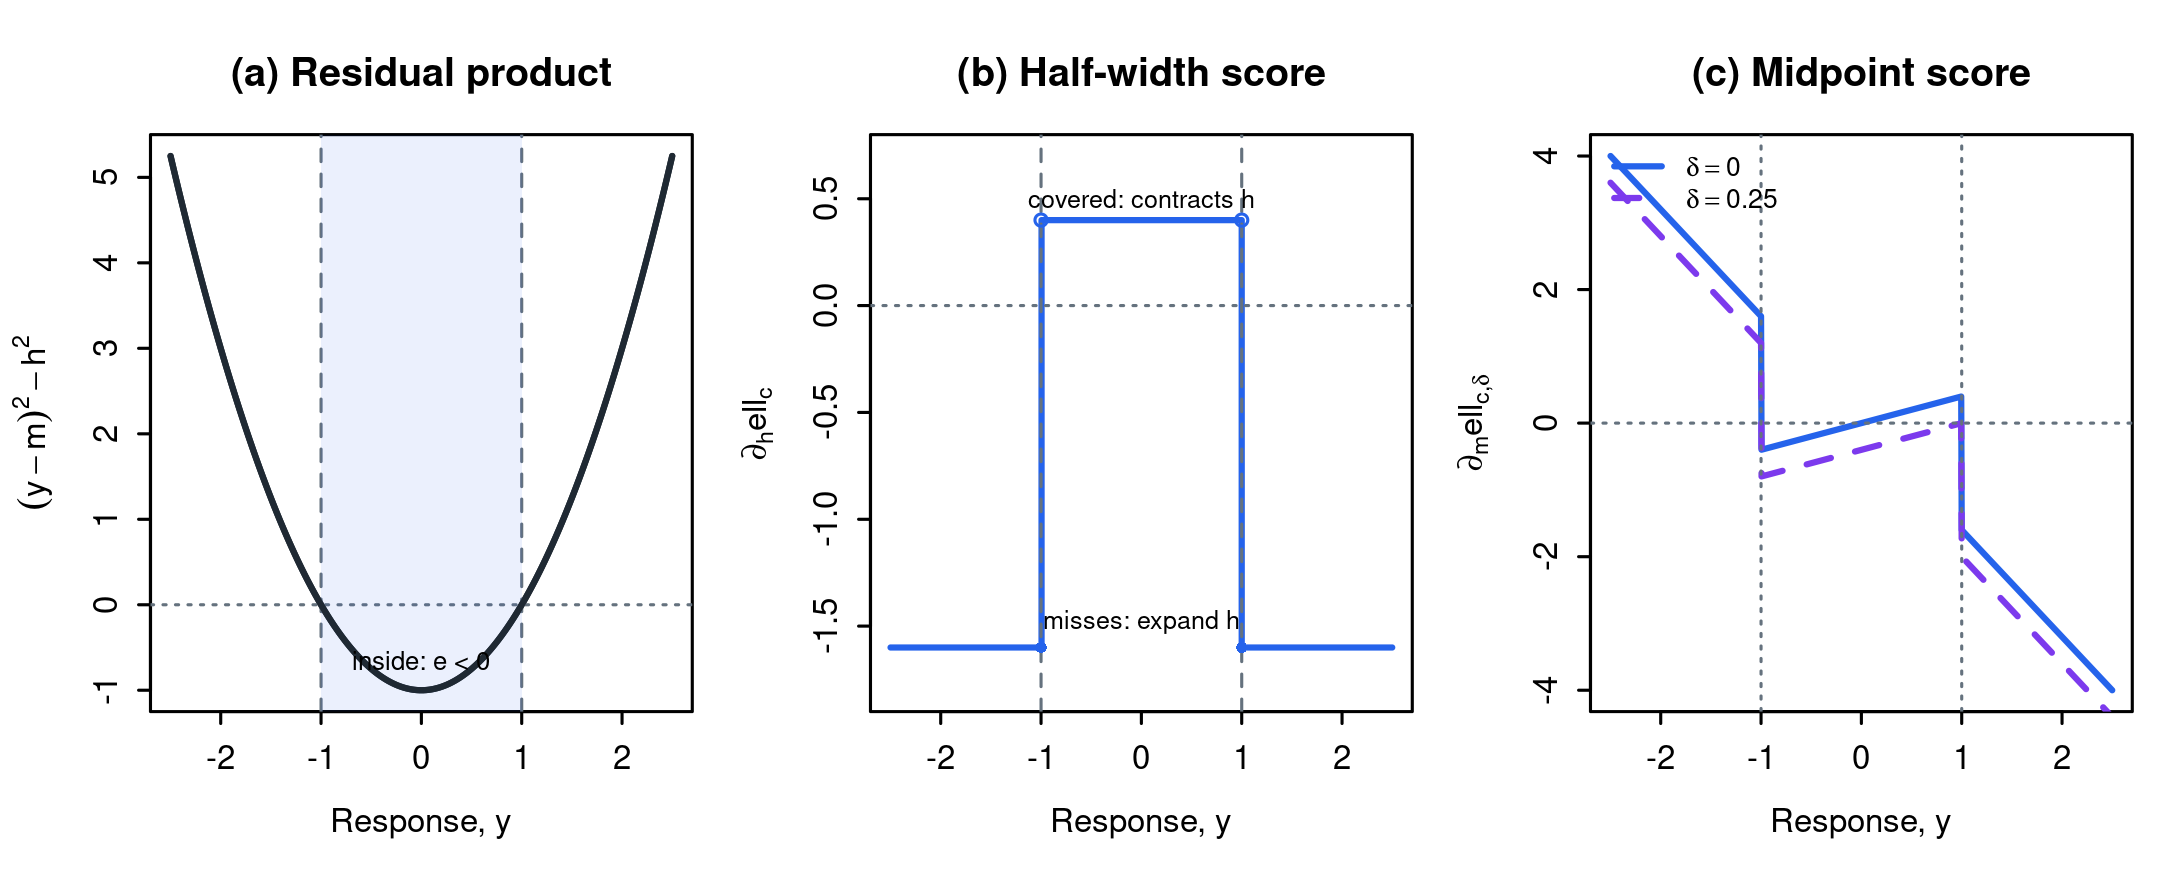
\includegraphics[width=\textwidth]{figures/ch05-mti/generated/figS02_loss_geometry.png}
\caption{\textbf{MPI loss geometry and the fixed midpoint tilt.}
For \(c=0.80\), \(m=0\), and \(h=1\), the residual product is negative exactly
inside the interval. The half-width score contracts \(h\) for covered
observations and expands it for misses. A fixed \(\delta\) adds a constant
shift to the midpoint score but leaves the half-width score unchanged. These
plots use the strict convention \(\ind(e<0)\): filled endpoint marks show the
score at \(y=\pm1\), while open marks show the one-sided inside limits. These
are deterministic pointwise score calculations, not fitted results.}
\label{rqr:fig:supp-loss-geometry}
\end{figure}

\section{Fixed-Target MTI-ECM Calculation}
\label{rqr:sec:supp-mti-ecm}

The MTI-ECM calculation used in the validation study is a deterministic mode
calculation for a fixed loss-defined target. It is included because it links the
tolerance comparison to the MTI generalized-Bayes construction. The calculation
updates an interval-root target under a loss; the distribution-free tolerance
guarantee comes from the TCSP scan calibration.

For \(e_i=(y_i-\eta_{1i})(y_i-\eta_{2i})\), the fixed-target MTI loss is
\[
L_{n,q,\delta}
=\sum_{i=1}^n\left[
\rho_q(e_i)-q\delta(\eta_{1i}+\eta_{2i}-2y_i)
\right],
\qquad
\rho_q(r)=r\{q-\ind(r<0)\}.
\]
With fixed learning rate \(\omega_{\mathrm R}\), the generalized-posterior
kernel is proportional to
\[
\exp\{-\omega_{\mathrm R}L_{n,q,\delta}(\theta)\}\pi_0(\theta).
\]
The validation calculations are intercept-only, so \(\theta=(a,b)\) before the
two roots are sorted into lower and upper endpoints.

The pseudo-asymmetric-Laplace representation gives a convenient quadratic
conditional calculation. Define
\[
\sigma_{\mathrm R}=\omega_{\mathrm R}^{-1},\qquad
\xi_q=\frac{1-2q}{q(1-q)},\qquad
\phi_q=\frac{2}{q(1-q)}.
\]
Then
\begin{align}
&\frac{q(1-q)}{\sigma_{\mathrm R}}
\exp\{-\rho_q(e_i)/\sigma_{\mathrm R}\}\notag\\
&\quad=\int_0^\infty
\Normal\!\left(e_i\mid\xi_qv_i,\phi_q\sigma_{\mathrm R}v_i\right)
\Exp\!\left(v_i\mid\mathrm{rate}=1/\sigma_{\mathrm R}\right)\,dv_i.
\label{rqr:eq:supp-pseudo-al-mixture}
\end{align}
The latent scale is computational; it augments a loss factor rather than a
sampling distribution for \(Y_i\).

Under the \(\GIG(\nu,A,B)\) convention proportional to
\(v^{\nu-1}\exp\{-(Av+B/v)/2\}\), the conditional scale law has
\[
v_i\mid\cdot\sim
\GIG\left\{
\frac12,\
\frac{1}{2\sigma_{\mathrm R}q(1-q)},\
\frac{q(1-q)e_i^2}{2\sigma_{\mathrm R}}
\right\}.
\]
For \(e_i\ne0\),
\[
\tau_i=E(v_i^{-1}\mid\cdot)=\frac{1}{q(1-q)|e_i|}.
\]
The numerical ECM calculation uses a small response-product scale floor when
\(e_i\) is near zero, objective backtracking after each accepted cycle, and
deterministic multi-start selection by the exact penalized objective.

\begin{algorithmblock}{Fixed-target MTI-ECM mode}
\begin{enumerate}[leftmargin=2.2em,itemsep=0.3em,parsep=0pt]
\item Fix \(q\), \(\delta\), \(\omega_{\mathrm R}\), the ridge prior precision,
and deterministic starting roots.
\item At the current roots, compute product residuals \(e_i\) and inverse-scale
moments \(\tau_i\), using the prespecified numerical floor only when needed.
\item Holding one root fixed, solve the Gaussian conditional maximization for
the other root. Repeat with the roles exchanged.
\item Accept a full cycle only if the exact penalized objective decreases,
using backtracking if necessary.
\item Return the best deterministic mode over the prespecified starting values,
then sort the two raw roots to report the interval.
\end{enumerate}
\end{algorithmblock}

The fitted content \(q\) and tilt \(\delta\) are not estimated as ordinary
parameters inside the generalized posterior. The validation study profiles over
a prespecified grid in a separate calibration step and then applies the selected
rule unchanged to independent replications.

\section{Direct DP Content Check}
\label{rqr:sec:supp-direct-dp-check}

The MTI-ECM comparator uses a model-based content-probability check during calibration.
For a fixed closed interval \(I=[l,u]\), let \(N_n(I)=\sum_{i=1}^n\ind(Y_i\in I)\).
Under the direct Dirichlet-process model
\[
F\sim\mathrm{DP}(a,H),\qquad
Y_i\mid F\stackrel{\mathrm{iid}}{\sim}F,
\]
with fixed \(a>0\) and fixed base distribution \(H\), conjugacy gives an exact
posterior law for the interval content.

\begin{proposition}[Direct DP fixed-interval content law]
\label{rqr:prop:supp-dp-content-law}
For fixed \(I=[l,u]\),
\[
F(I)\mid D_n\sim
\mathrm{Beta}\{aH(I)+N_n(I),a(1-H(I))+n-N_n(I)\}.
\]
Consequently \(p_n(I;c)=\Pr\{F(I)\ge c\mid D_n\}\) is available from a Beta
survival probability.
\end{proposition}

\begin{proof}
Dirichlet-process conjugacy gives
\[
F\mid D_n\sim \mathrm{DP}(a+n,H_n),\qquad
H_n=\frac{aH+\sum_{i=1}^n\delta_{Y_i}}{a+n}.
\]
For the partition \((I,I^c)\), the finite-dimensional distribution of a
Dirichlet process is Dirichlet with parameters
\((a+n)H_n(I)=aH(I)+N_n(I)\) and
\((a+n)H_n(I^c)=a\{1-H(I)\}+n-N_n(I)\). The first coordinate is the stated
Beta distribution.
\end{proof}

The direct DP check is used only to choose eligible MTI-ECM candidates in the
calibration run. The distribution-free tolerance guarantee in this paper comes
from the TCSP retained-count calibration.

\section{Calibrated Minimum-Width Tolerance Intervals}
\label{rqr:sec:tcsp}

The preceding theory fixes population content and interval placement. A
tolerance interval adds a repeated-sampling requirement. For iid continuous
univariate observations, the target statement is
\[
\Pr_F^n\{C_F(\widehat T_n)\ge c\}\ge 1-\alpha,\qquad
C_F([L,U])=F(U)-F(L),
\]
where \(\widehat T_n\) is a data-dependent interval. Six quantities must be
kept distinct. The required population content is \(c\), and the tolerance
confidence is \(1-\alpha\). The scan calibration returns a retained count
\(k\), so the fitted content used by a fixed-target MTI approximation is
\(q=k/n\). The fixed MTI placement tilt is \(\delta\), and the
generalized-Bayes learning rate is \(\omega_{\mathrm R}\). When a separate
response-distribution model for \(F\) is used, \(1-\gamma\) denotes a posterior
content-probability threshold for eligible intervals. Neither \(\omega_{\mathrm R}\) nor
\(1-\gamma\) determines the tolerance confidence.
In this article, TCSP denotes the tolerance-calibrated shortest-path procedure:
first calibrate a retained count by the scan statistic, then report the
shortest closed empirical window at that count.

\paragraph{Scan-calibrated empirical procedure.}
Let \(Y_{(1)}\le\cdots\le Y_{(n)}\). For content \(c\), define the uniform scan
statistic
\[
M_n(c)=\max_{0\le s\le 1-c}\#\{i:U_i\in[s,s+c]\},
\qquad U_i\stackrel{\mathrm{iid}}{\sim}\mathrm{Unif}(0,1).
\]
The calibrated retained count is
\[
k_{n,c,\alpha}
=\min\{k:\Pr(M_n(c)<k)\ge 1-\alpha\}.
\]
This count is fixed before any endpoint model is fit. The reported empirical
interval is the closed order-statistic window
\[
\widehat T_n=
[Y_{(\widehat j)},Y_{(\widehat j+k-1)}],
\qquad
\widehat j=\min\argmin_{1\le j\le n-k+1}
\{Y_{(j+k-1)}-Y_{(j)}\},
\]
with \(k=k_{n,c,\alpha}\). This convention is closed and contains exactly
\(k\) sample observations under continuity. It differs from the half-open
\((Y_{(j)},Y_{(j+k)}]\) convention sometimes used for order-statistic
tolerance limits, so a result proved for one convention cannot be transferred
without reconciling the indices and endpoint rule.

\paragraph{MTI summaries after selection.}
The selected window also defines a fixed-target MTI approximation for endpoint
uncertainty. Its fitted content and content buffer are
\[
q_{n,c,\alpha}=k_{n,c,\alpha}/n,\qquad
t_{n,c,\alpha}=q_{n,c,\alpha}-c.
\]
The empirical shortest-path tilt is
\[
\widehat\delta_{\mathrm{SH}}(q)
=
\frac1k\sum_{\ell=\widehat j}^{\widehat j+k-1}Y_{(\ell)}
-\frac1n\sum_{i=1}^nY_i.
\]
After \(q\) and \(\widehat\delta_{\mathrm{SH}}\) are fixed, an MTI endpoint
model with parameter block \(\theta\) uses the loss-based update
\[
\pi_{q,\delta,\omega_{\mathrm R}}(\theta\mid D_n)
\propto
\exp\{-\omega_{\mathrm R}L_{q,\delta,n}(\theta)\}\pi_0(\theta).
\]
This generalized posterior quantifies uncertainty about a fixed interval-root
functional after the target has been specified. The tolerance interval remains
the empirical order-statistic window \(\widehat T_n\). Because
\(\widehat\delta_{\mathrm{SH}}\) is computed from the same sample, these
posterior summaries are conditional on the selected target and do not propagate
shortest-window selection uncertainty. An unconditional interpretation requires
a plug-in stability theorem or a separate target-selection sample.

\paragraph{Additional extensions.}
Response-distribution Bayesian shortest-interval calculations and sample-split spacing constructions
are useful extensions, but they answer different evidentiary questions from the
primary TCSP procedure. A response-distribution model gives posterior
content probabilities under a model for \(F\), whereas TCSP supplies a
distribution-free scan-calibrated empirical interval. A split-spacing construction
uses independent target-selection and calibration samples, whereas TCSP uses the full
sample to choose the minimum-width calibrated order-statistic window. These
extensions remain available as separate methodological and proof directions;
they are not part of the main validation comparison.

\paragraph{Numerical calibration and proof guarantees.}
Numerical evaluation of \(k_{n,c,\alpha}\) is consequential because it sets the
reported interval. The calculation uses adaptive Monte Carlo
calibration of the uniform scan distribution. At each look, one-sided
Clopper--Pearson lower bounds are Bonferroni-adjusted over feasible retained
counts and adaptive looks, and the first retained count whose lower confidence
bound reaches \(1-\alpha\) is selected. The full-range interval
uses its exact order-statistic probability. A more conservative
Massart--DKW empirical-CDF lower band remains available as a conservative
alternative
\citep{rqr-Massart1990DKW}. Exact scan recursion remains an open numerical task.
Accordingly, exact critical-count calculation and the finite-sample theorem for
this closed-window rule are treated as open proof and numerical-calibration
tasks.

The available theory is deliberately narrower than the computational procedures.
Theorems~\ref{rqr:thm:quantile-window}--\ref{rqr:thm:profiled-mean-tilt} identify
the fixed-content MTI family and its admissible tilt coordinate. For tolerance
inference, the empirical closed order-statistic window is the reported interval;
generalized-posterior summaries for fixed \((q,\delta)\) describe endpoint-root
uncertainty after a target has been specified and do not serve as the
content--confidence guarantee. Split exact-spacing calibration has an exact
conditional iid univariate Beta law. The scan count is selected by the
adaptive Clopper--Pearson numerical procedure above, with numerical confidence
distinguished from tolerance confidence. Direct DP and Gaussian DPM
intervals are ordinary
response-distribution Bayesian alternatives, not MTI generalized posteriors.
Exact scan recursion, a finite-sample proof matched to the closed-window
convention, selected-interval asymptotics, posterior-to-interval transfer,
and regression-family tolerance calibration remain separate open problems.

\paragraph{Shortest-path continuation.}
The population shortest-window path gives useful continuation geometry for
moving across contents. This geometry helps initialize and check numerical
paths; it is not the scan calibration. Suppose that the density is
differentiable and strictly unimodal,
and that the shortest window
\(I_q=[L_q,U_q]=[Q(u_q),Q(u_q+q)]\) is unique and interior over a range of
\(q\). Equal endpoint densities then satisfy
\[
f(L_q)=f(U_q)=\lambda_q.
\]
Writing \(a_q=f'(L_q)>0\) and \(b_q=f'(U_q)<0\), formal differentiation of
the content and equal-density equations gives
\[
L_q'=\frac{b_q}{\lambda_q(a_q-b_q)}<0,
\qquad
U_q'=\frac{a_q}{\lambda_q(a_q-b_q)}>0.
\]
Thus the first-order shares of added probability assigned to the left and
right boundaries are
\[
p_L(q)=\frac{-b_q}{a_q-b_q},\qquad
p_R(q)=\frac{a_q}{a_q-b_q},\qquad
p_L(q)+p_R(q)=1.
\]
Only under local symmetry are the two shares equal to one half. The width
satisfies
\[
W_{\mathrm{SH}}'(q)=\frac{1}{\lambda_q},
\qquad
W_{\mathrm{SH}}''(q)
=-\frac{a_qb_q}{\lambda_q^3(a_q-b_q)}>0.
\]
Hence additional content becomes increasingly expensive as the endpoints move
into lower-density regions. If
\(m_q=q^{-1}\int_{u_q}^{u_q+q}Q(s)\,ds
=\mu+\delta_{\mathrm{SH}}(q)\), then
\[
\delta_{\mathrm{SH}}'(q)
=\frac{p_L(q)L_q+p_R(q)U_q-m_q}{q}.
\]
These derivative calculations motivate numerical continuation and diagnose
its behavior. Full regularity, boundary, and nonuniqueness arguments are
reserved for a formal shortest-path theorem.

The continuation calculation starts from a globally solved content, predicts
each next window by nested expansion of the previous window, applies local
correction in a neighborhood of the current solution, expands the neighborhood
when the local optimum lands on its boundary, and finally verifies the selected
interval by an exhaustive empirical scan. The exhaustive scan, not the
continuation approximation, defines the selected window. The continuation
argument does not cover infeasible calibration
\((k>n)\), ties or atoms that violate the continuous-sample convention,
nonunique shortest windows, response-scale dependence of geometric width, and
unsupported attempts to attach the scan guarantee to posterior summaries.

The construction therefore separates three quantities: the empirical scan
tolerance interval, the full-distribution Bayesian shortest-interval
uncertainty summaries, and the fixed-target MTI generalized-posterior summaries.
Finite-sample scan validity requires a proof matched to the closed-window rule
and a calibrated critical count;
first-order tolerance or population-reference width statements additionally require
same-sample shortest-window asymptotics. Any transfer from posterior content
probabilities to endpoint coverage, or from fixed-target MTI summaries to
the selected shortest interval, requires a separate equivalence or
direct-calibration result. Tolerance confidence comes from the scan calibration,
and \(\omega_{\mathrm R}\) remains the generalized-Bayes learning rate.

\section{Width-Regularized Interval Loss}
\label{rqr:sec:supp-rqr-w}

The width-regularized variant in \citet{rqr-PouplinEtAl2024RQR} has a different
population score system from the MPI loss. For comparison, they use the RQR-W
population objective
\[
\E\left[\rho_q\{(Y-a)(Y-b)\}\right]
+\frac{\lambda_W}{2}(b-a)^2,
\qquad \lambda_W\ge0.
\]
In the present terminology, RQR-W is a width-regularized modification of the
MPI loss, not the MPI loss itself.
At a nondegenerate interior stationary point, subtracting the two endpoint
score equations gives
\[
\Pr(a<Y<b)=q-2\lambda_W.
\]
Thus \(q=c+2\lambda_W\) restores content \(c\), subject to
\(0\le\lambda_W<(1-c)/2\). The midpoint equation then gives
\[
\E(Y\mid a<Y<b)
=\mu+\frac{2\lambda_W}{c}(\mu-m),
\qquad m=\frac{a+b}{2}.
\]
Except in special symmetric cases, RQR-W therefore changes the
mean-preserving placement equation. It is a coverage-corrected compromise
between MPI risk and squared width, not a tie-breaker among
unidentified MPI minimizers.

More generally, if a differentiable width penalty \(P(w)\), \(w=b-a\), is
added to a check loss at level \(q\), the coverage equation is
\[
\Pr(a<Y<b)=q-\frac{2P'(w)}{w}.
\]
A correction independent of the distribution and realized width is possible
only when \(P'(w)/w\) is constant, which yields a quadratic penalty up to an
additive constant. This explains both the form of RQR-W and why its path does
not generally coincide with the shortest-contiguous path.

\section{Validation Design}
\label{rqr:sec:evaluation}

Validation is reserved for questions that require repeated sampling or
held-out comparison. Population calculations verify the fixed-content and
mean-tilt characterizations without Monte Carlo error. Reference calculations
compare generalized-posterior draws with quadrature, dense Gaussian full
conditionals, analytic scale updates, and restart equivalence. These
checks provide numerical evidence for the stated computational target on
reference problems. Empirical coverage, width efficiency, and comparator
ranking require repeated-sampling validation.

The main tolerance study is prespecified before inspecting comparative results,
following simulation-study reporting principles
\citep{rqr-MorrisWhiteCrowther2019Simulation}. It uses iid continuous samples from
eight centered and scaled simulation distributions. Gaussian and Student \(t_3\)
samples serve as symmetric reference distributions. The asymmetric simulation
distributions are exponential,
asymmetric Laplace with \(\tau=0.10\), a two-piece Normal law with scale ratio
\(1{:}12\), Beta\((1,8)\), Gamma\((0.5,1)\), and log-normal with log-scale
standard deviation \(1.25\). This panel is intentionally skewed toward
asymmetric laws because the theoretical advantage of a shortest calibrated
window is most relevant when equal-tail or full-range behavior is inefficient.
Multimodal cases are excluded because none of the reported methods is designed
to recover disconnected high-density regions.
The primary simulation design fixes tolerance confidence at \(0.95\) and uses 1000
paired replications per simulation distribution and feasible cell.
The feasible cells are \(n=50,c=0.90\), \(n=100,c\in\{0.90,0.95\}\), and
\(n\in\{500,1000\},c\in\{0.90,0.95,0.99\}\).

The small-sample restriction is structural. For a two-sided distribution-free
interval, even the full sample range reaches content \(c\) with confidence
\(0.95\) only when
\[
  1-n(1-c)c^{n-1}-c^n \ge 0.95 .
\]
The corresponding minimum sample sizes are \(46\), \(93\), and \(473\) for
\(c=0.90\), \(0.95\), and \(0.99\), respectively. Thus
\(n=50,c=0.95\) and \(n=100,c=0.99\) are excluded from the confirmatory
comparison because no two-sided distribution-free method can support the
requested statement in those cells. The \(c=0.99\) rows begin at \(n=500\), the
nearest rounded sample size above the \(n=473\) threshold.

The comparison is deliberately narrow. TCSP is the primary scan-calibrated
shortest empirical tolerance procedure. The reported TCSP calculations use the
adaptive Clopper--Pearson scan calibration described above. Its optimality is
class-specific: it minimizes width among closed
order-statistic windows satisfying the calibrated retained-count rule.
The MTI-ECM comparator links the validation study to the generalized-Bayes
interval construction. It uses a prespecified adaptive calibration rule indexed
by sample size and requested content. Within each cell, the rule fixes a direct
Dirichlet-process content-probability check from an independent calibration run, profiles
fixed-target MTI-ECM endpoint fits over fitted content and retained-mean tilt,
and keeps the shortest candidate satisfying the content-probability check and a
same-cell width-stability restriction against TCSP. This empirical validation is
separate from the distribution-free scan theorem that supports TCSP.
Young--Mathew interpolation
\citep{rqr-YoungMathew2014NonparametricTolerance} and Wilks min--max intervals
\citep{rqr-Wilks1941ToleranceLimits,rqr-Wilks1942StatisticalPrediction} provide the
classical order-statistic comparators. The primary metric is the
content-attainment rate: the Monte Carlo estimate of
\(\Pr_F^n\{C_F(\widehat T_n)\ge c\}\), where
\(C_F([L,U])=F(U)-F(L)\). For each replication, this content check uses the
known simulation distribution rather than the fraction of sampled observations
inside the produced interval. If a method produced no interval in a replication,
that replication would be counted as nonattainment. Widths are reported as
distribution-level empirical 2.5\%--97.5\% ranges, avoiding width averages
across distributions with different scales and tail behavior.
Figure~\ref{rqr:fig:tolerance-validation-width-ranges} also marks the population
shortest content-\(c\) interval for each simulation law. This benchmark uses
the known distribution and serves as a lower width reference rather than as a
sample-based tolerance procedure.

\begin{table}[!htbp]
\centering
\caption{\textbf{Independent-sample tolerance validation.} Results are shown by
feasible sample-size/content cell and method. Each row summarizes the range
across eight simulation distributions at tolerance confidence \(0.95\). All four
reported methods produced an interval in every replication in this run.}
\label{rqr:tab:tolerance-validation-primary}
\TableStyle
\begin{tabular}{@{}l@{\hspace{0.75em}}l@{\hspace{0.75em}}r@{}}
\toprule
Cell & Method & Content-attainment range (\%)\\
\midrule
\(n=50,c=0.90\) & TCSP & 95.6--97.7 \\
 & MTI-ECM & 95.8--97.8 \\
 & Young--Mathew & 94.6--97.0 \\
 & Wilks & 95.6--97.7 \\
\addlinespace[0.25em]
\(n=100,c=0.90\) & TCSP & 98.3--99.4 \\
 & MTI-ECM & 98.5--99.7 \\
 & Young--Mathew & 95.2--96.9 \\
 & Wilks & 99.9--100.0 \\
\addlinespace[0.25em]
\(n=100,c=0.95\) & TCSP & 96.2--97.3 \\
 & MTI-ECM & 95.1--97.5 \\
 & Young--Mathew & 95.5--96.8 \\
 & Wilks & 96.2--97.3 \\
\addlinespace[0.25em]
\(n=500,c=0.90\) & TCSP & 96.7--99.0 \\
 & MTI-ECM & 97.3--99.7 \\
 & Young--Mathew & 94.4--96.1 \\
 & Wilks & 100.0 \\
\addlinespace[0.25em]
\(n=500,c=0.95\) & TCSP & 96.2--99.1 \\
 & MTI-ECM & 97.0--99.2 \\
 & Young--Mathew & 94.2--96.6 \\
 & Wilks & 100.0 \\
\addlinespace[0.25em]
\(n=500,c=0.99\) & TCSP & 95.3--96.7 \\
 & MTI-ECM & 95.2--97.4 \\
 & Young--Mathew & 95.1--96.7 \\
 & Wilks & 95.3--96.7 \\
\addlinespace[0.25em]
\(n=1000,c=0.90\) & TCSP & 98.0--99.6 \\
 & MTI-ECM & 97.7--99.5 \\
 & Young--Mathew & 94.2--96.6 \\
 & Wilks & 100.0 \\
\addlinespace[0.25em]
\(n=1000,c=0.95\) & TCSP & 97.6--99.6 \\
 & MTI-ECM & 96.7--99.9 \\
 & Young--Mathew & 95.1--96.3 \\
 & Wilks & 100.0 \\
\addlinespace[0.25em]
\(n=1000,c=0.99\) & TCSP & 97.5--99.5 \\
 & MTI-ECM & 97.9--99.4 \\
 & Young--Mathew & 94.1--97.2 \\
 & Wilks & 99.9--100.0 \\
\bottomrule
\end{tabular}

\end{table}

\begin{figure}[!htbp]
\centering
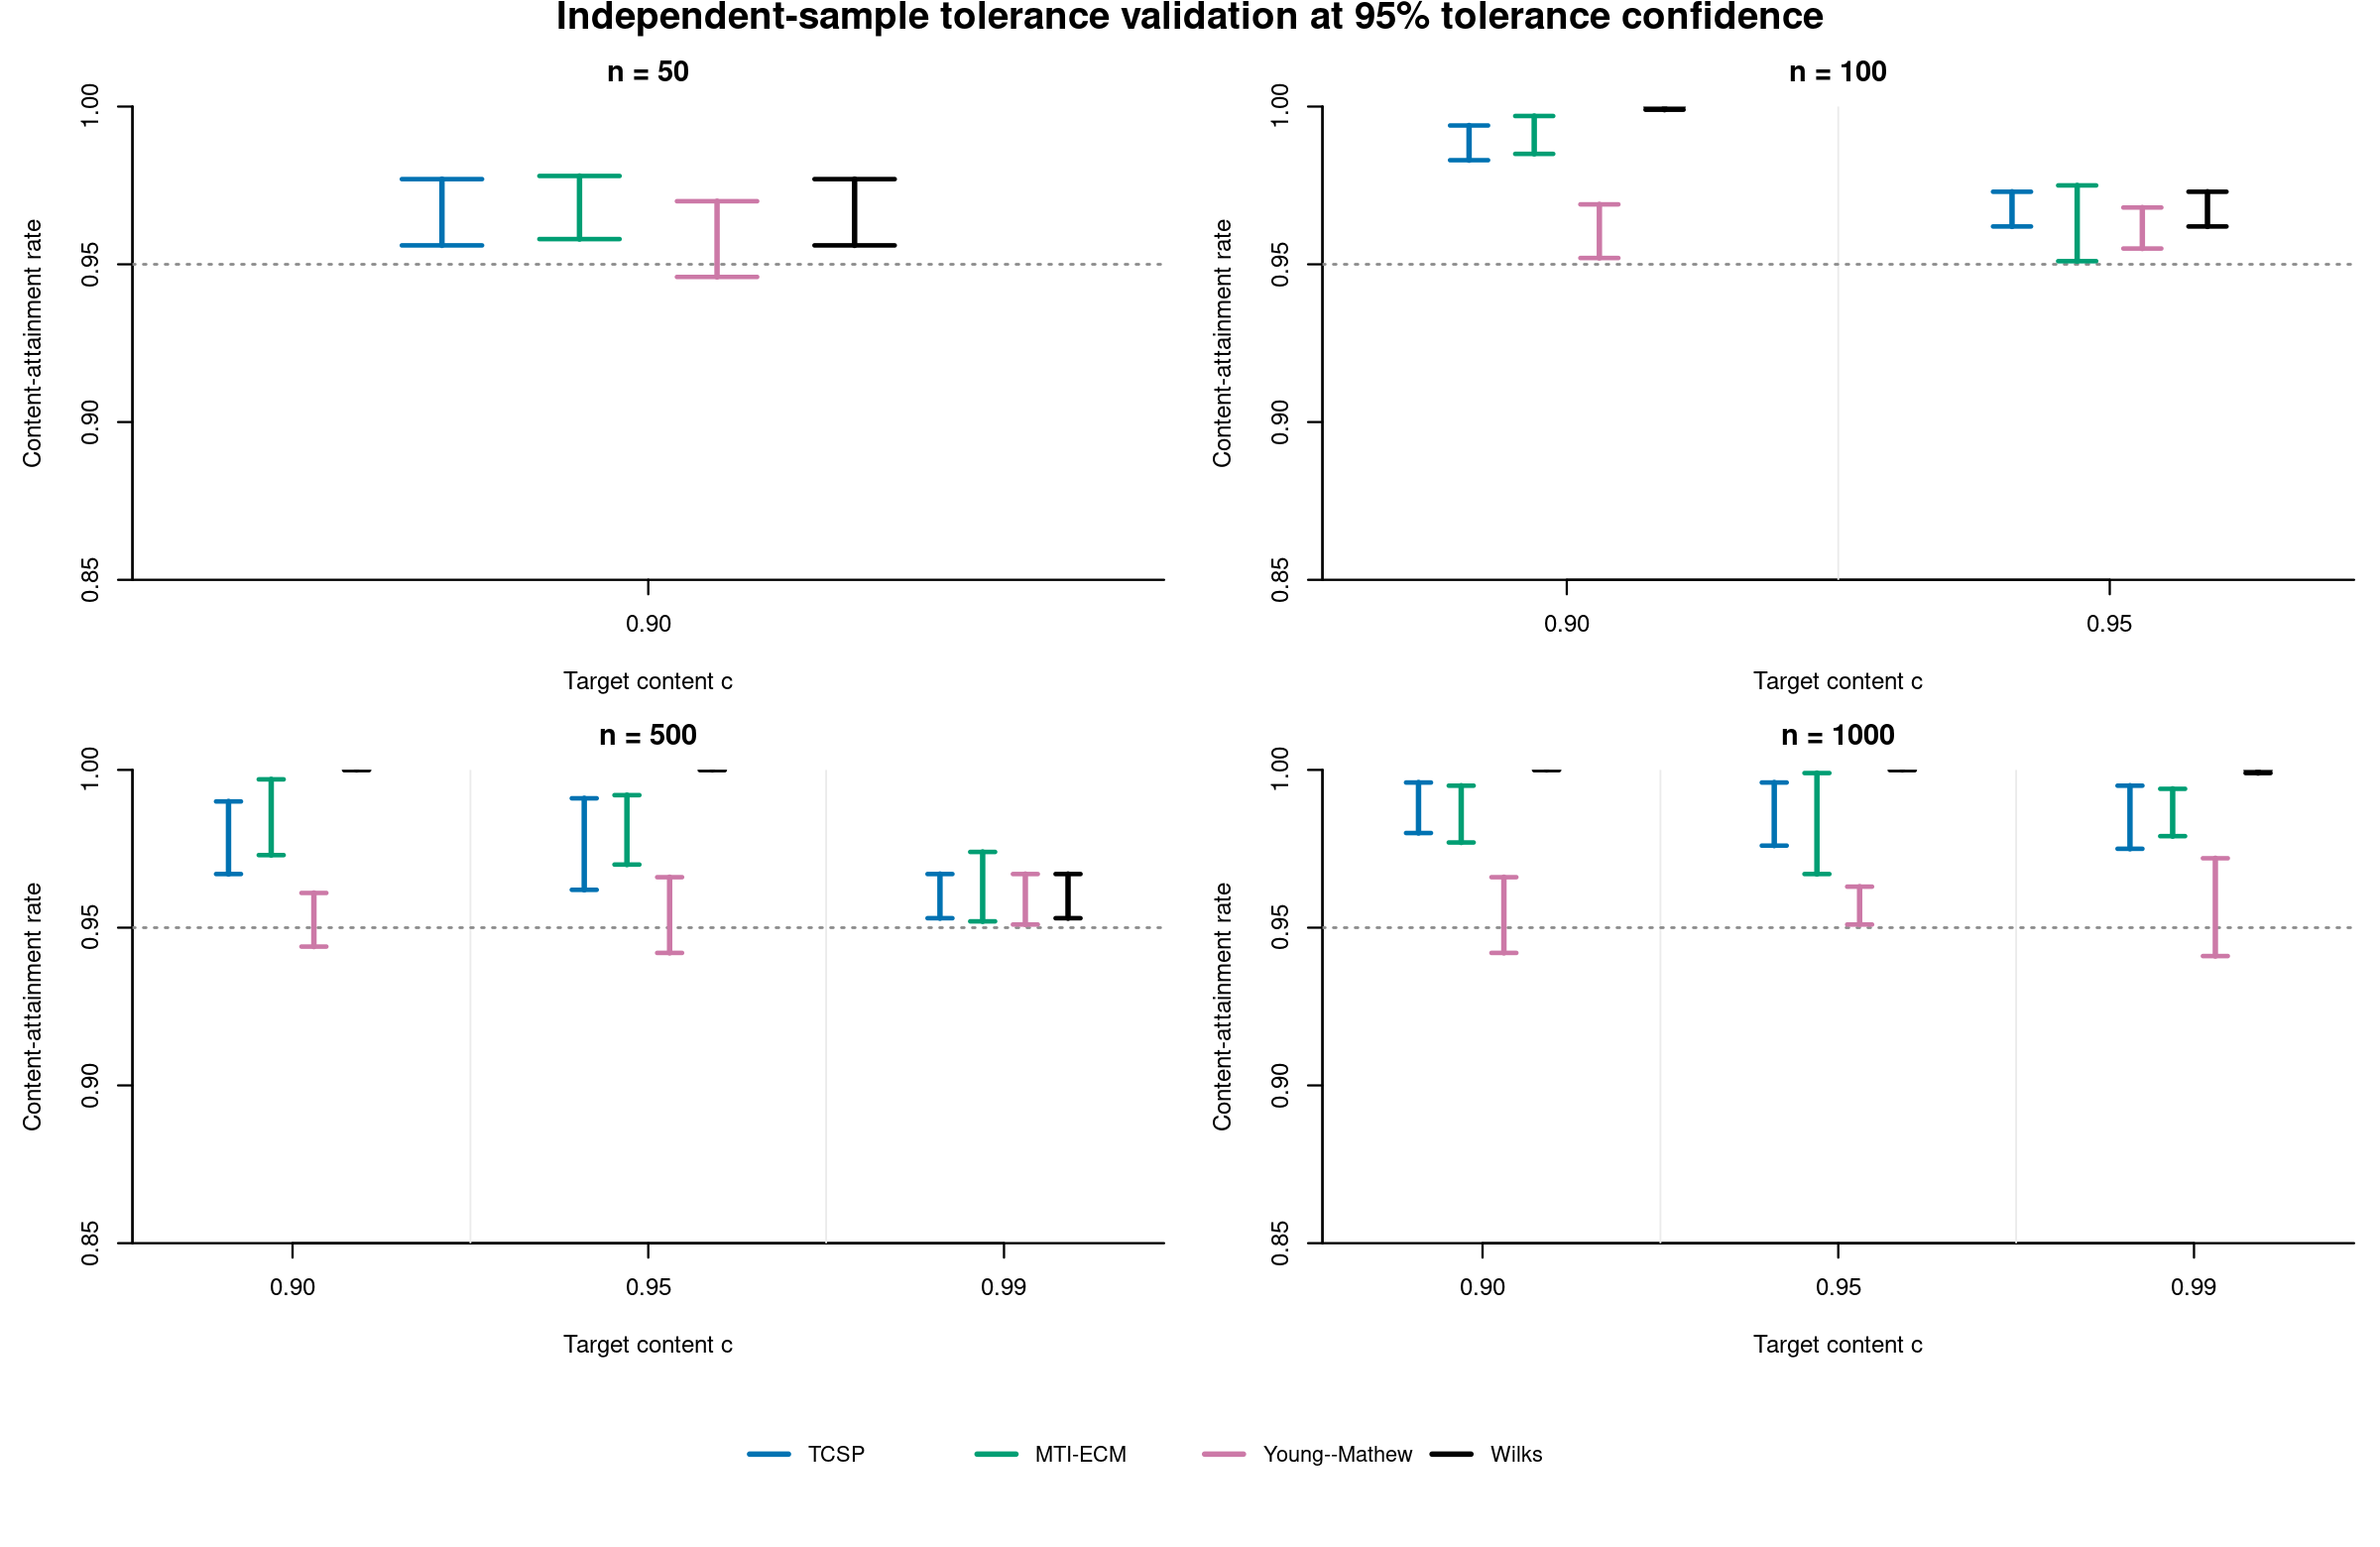
\includegraphics[width=\textwidth]{figures/ch05-mti/generated/fig04_tolerance_validation_primary.png}
\caption{\textbf{Content-attainment by sample size and target content.}
Intervals not produced are counted as nonattainment.
Vertical intervals in the content-attainment panels show the range across
distributional scenarios, and the axis is zoomed to \(0.85\)--\(1.00\).
Dashed reference lines mark nominal tolerance confidence \(0.95\).}
\label{rqr:fig:tolerance-validation-primary}
\end{figure}

\begin{figure}[!htbp]
\centering
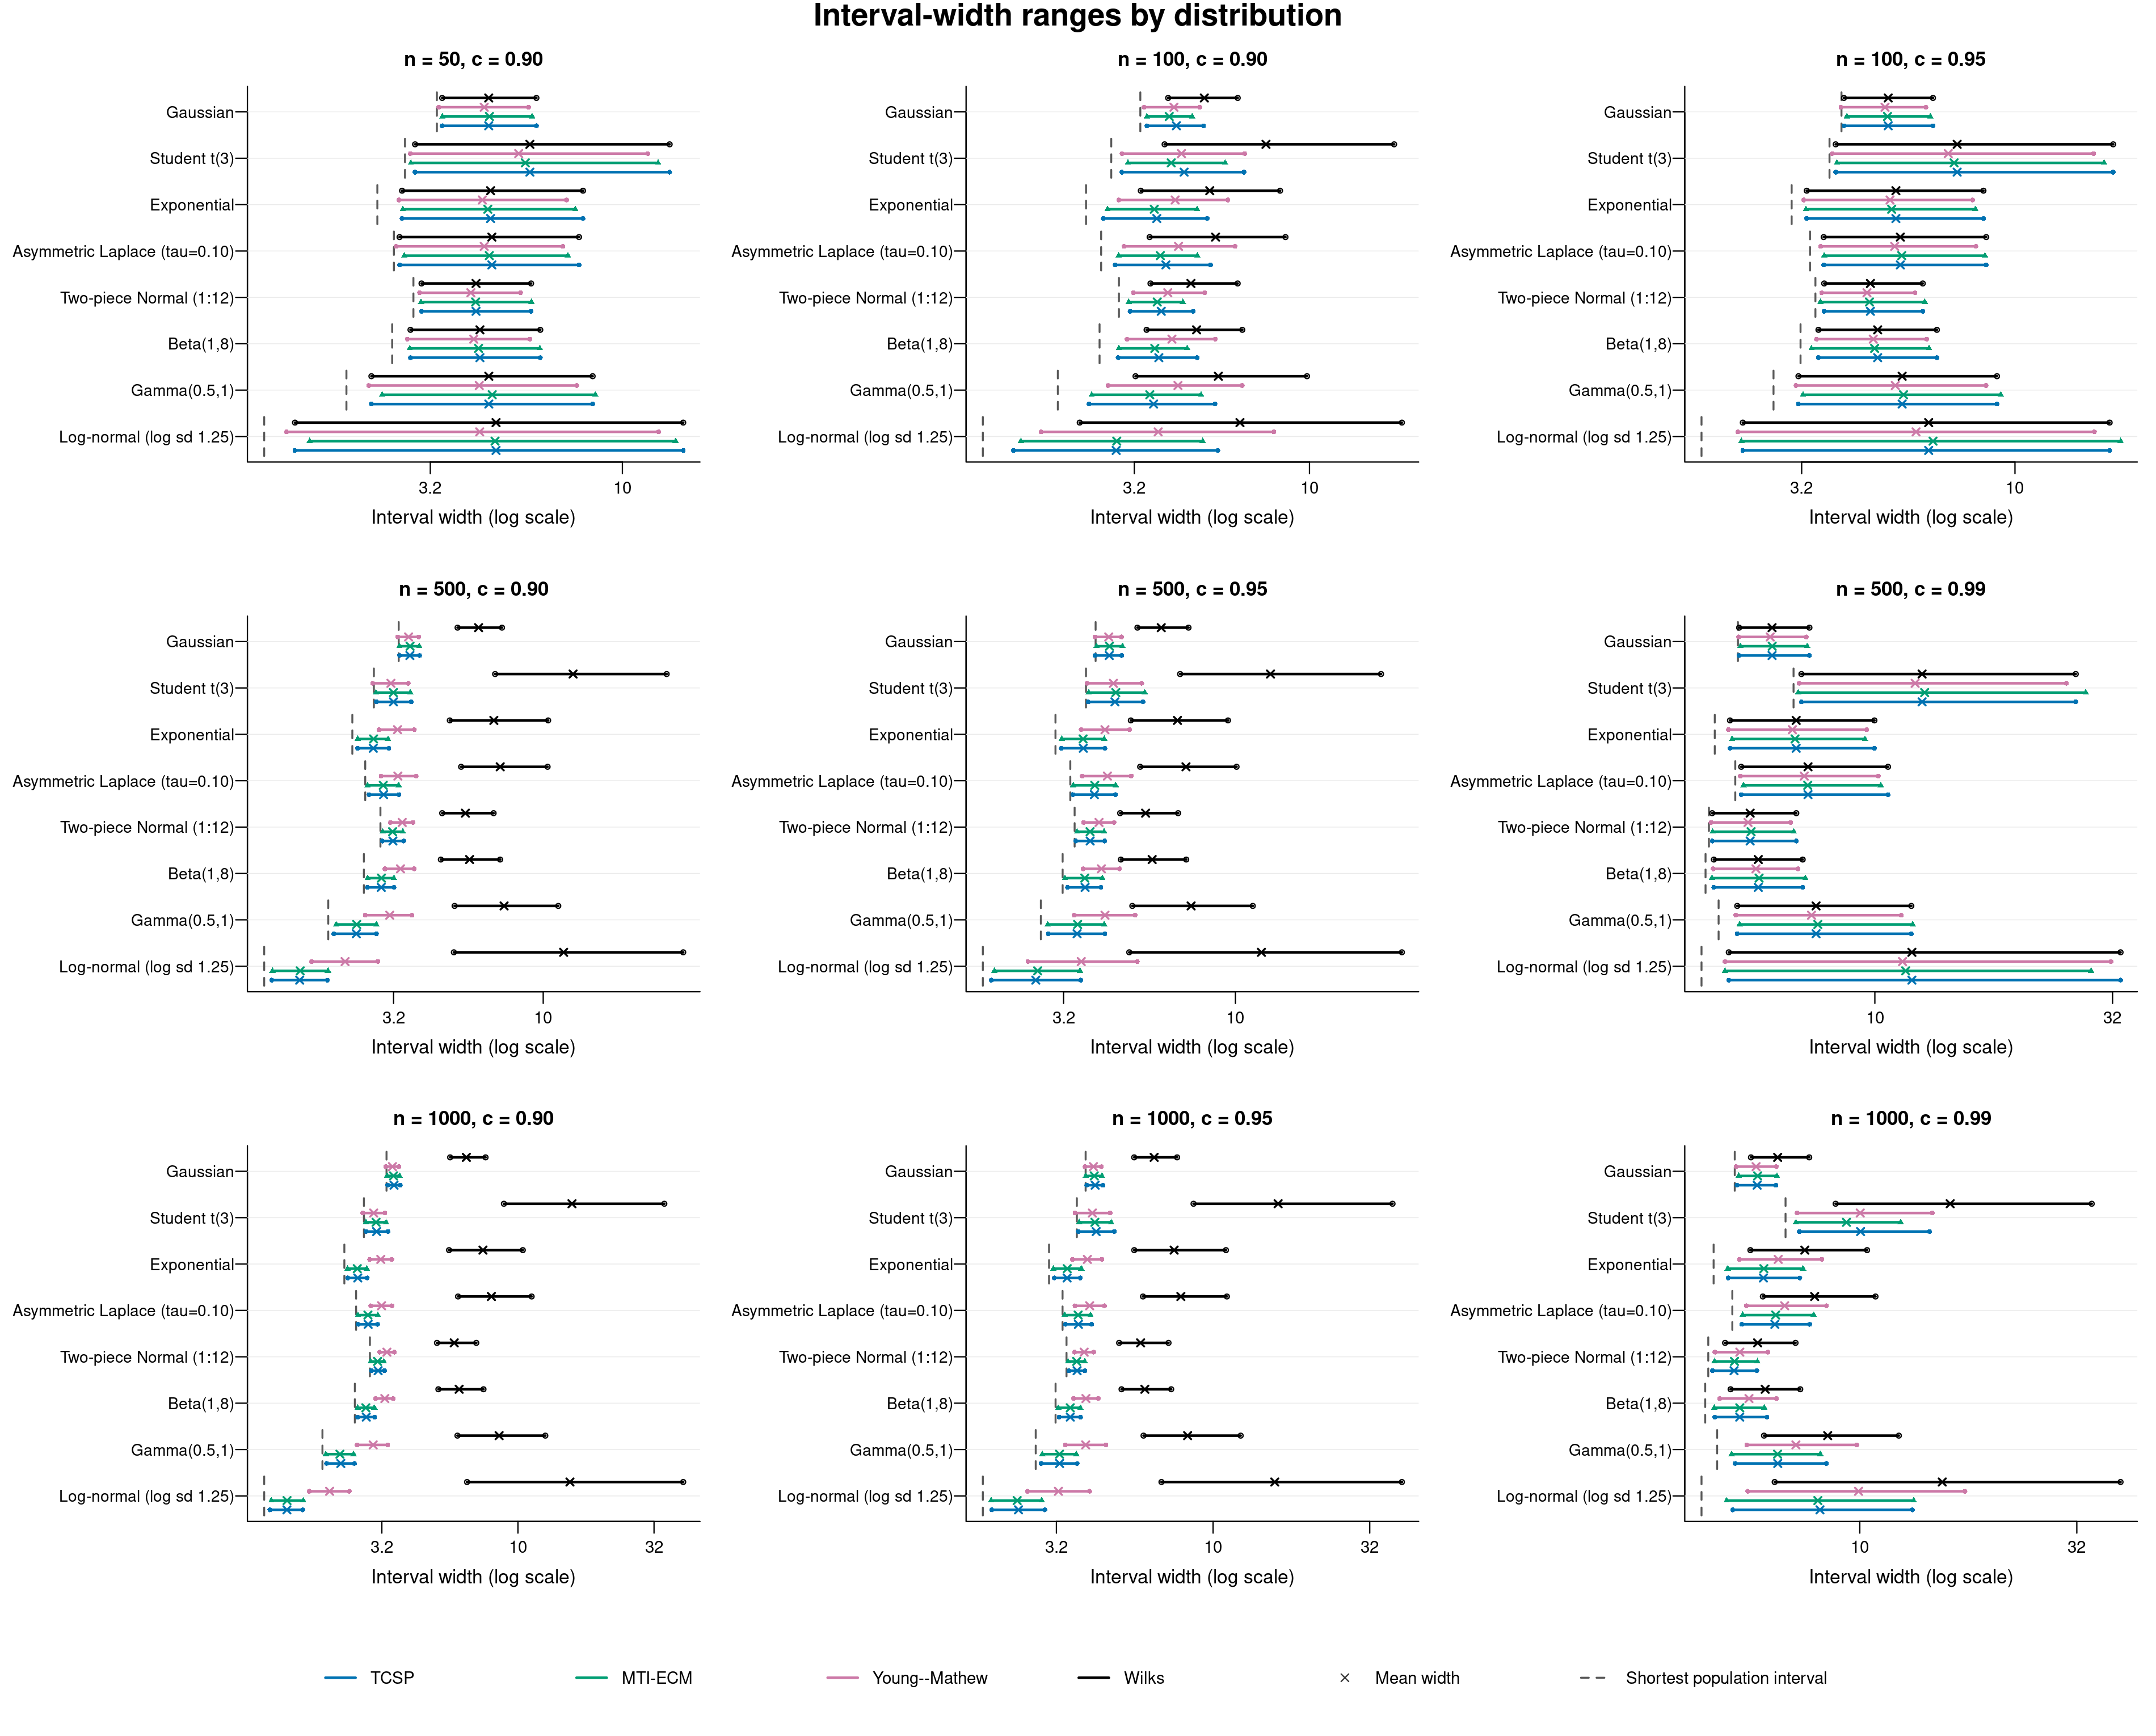
\includegraphics[width=\textwidth]{figures/ch05-mti/generated/fig05_tolerance_validation_width_ranges.png}
\caption{\textbf{Interval-width ranges by distribution.} Horizontal intervals show empirical
2.5\%--97.5\% ranges of interval lengths within each distribution,
sample-size/content cell, and method. Crosses mark the mean interval width
across the 1000 paired replications. Dashed gray markers show the corresponding
population shortest content-\(c\) interval widths under the known simulation
laws. The horizontal axis is logarithmic to display light-tailed, heavy-tailed,
and strongly skewed cases in one figure; the values remain raw interval
lengths.}
\label{rqr:fig:tolerance-validation-width-ranges}
\end{figure}

In the completed run, TCSP content-attainment ranges from 95.3\% to 99.6\% across
distribution-level cells, compared with 95.1\% to 99.9\% for MTI-ECM,
94.1\% to 97.2\% for Young--Mathew, and 95.3\% to 100.0\% for Wilks.
Figures~\ref{rqr:fig:tolerance-validation-primary}
and~\ref{rqr:fig:tolerance-validation-width-ranges} show the same comparison without
pooling widths across distributional scenarios. The calibrated scan procedure
targets the requested finite-sample statement directly. In the independent
validation run, the selected adaptive MTI-ECM rule has observed content
attainment above the nominal tolerance confidence in every distribution-level
cell. MTI-ECM provides a less conservative
width-seeking comparison tied to the generalized-Bayes interval construction:
it also stays above nominal tolerance confidence in all 72 distribution-level
cells and has a smaller cellwise median width than TCSP in 38 cells. The closest
independent validation cells remain near the nominal boundary, so this evidence
should be read as repeated-sampling validation of the selected MTI-ECM rule
rather than as a distribution-free finite-sample guarantee. Young--Mathew is
a strong nonparametric comparator and is slightly
shorter on the symmetric reference distributions, but it falls below nominal
tolerance confidence in nine skewed or heavy-tailed cells. In the six
asymmetric simulation distributions, TCSP and MTI-ECM are each shorter than
Young--Mathew in 36 of 54 cells. Wilks is simple and reliable, but it is often
much wider when the scan calibration does not force the full sample range.

The integrated material gives the distribution-level content-attainment and width tables behind these
summaries, the selected MTI-ECM calibration summary, the TCSP retained counts,
and the full-range feasibility thresholds used to choose the simulation design.
The excluded small-sample cells fall outside the region where a two-sided
distribution-free tolerance statement can be supported at confidence \(0.95\).
Other variants are kept outside the primary comparison.

\section{Tolerance-Validation Protocol and Feasibility}
\label{rqr:sec:supp-tolerance-validation-protocol}

The primary tolerance validation is restricted to iid continuous univariate
samples. This is the setting in which the scan-calibrated empirical procedure,
the stability-restricted MTI-ECM profile rule, Young--Mathew interpolation, and
Wilks-style full-range intervals can be compared on the same target. TCSP
is the primary calibrated tolerance procedure
because it selects the shortest closed order-statistic window at the calibrated
retained count. The reported TCSP calculations use adaptive Clopper--Pearson scan
calibration directly. The MTI-ECM comparator
profiles fixed-target endpoint fits over fitted content and retained-mean tilt,
then applies a direct Dirichlet-process fixed-interval content probability
threshold and a width-stability restriction. Young--Mathew and Wilks are included as classical order-statistic
comparators. Regression and dynamic tolerance calibration require additional
results because the fitted intervals vary with covariates or time.

The simulation design fixes tolerance confidence \(1-\alpha=0.95\) and uses
explicit feasible design cells:
\[
  \begin{aligned}
  (n,c)\in\{&
  (50,0.90),(100,0.90),(100,0.95),\\
  &(500,0.90),(500,0.95),(500,0.99),\\
  &(1000,0.90),(1000,0.95),(1000,0.99)\}.
  \end{aligned}
\]
The distributional panel contains two symmetric reference distributions and six
asymmetric simulation distributions. The symmetric reference distributions are
Gaussian and Student \(t_3\). The asymmetric simulation distributions are
exponential, asymmetric Laplace with \(\tau=0.10\), two-piece Normal with scale
ratio \(1{:}12\), Beta\((1,8)\), Gamma\((0.5,1)\), and log-normal with
log-scale standard deviation \(1.25\). All laws are centered and scaled before
sampling. Each cell uses paired random samples across methods. The
reproducibility materials include the code version, simulation settings,
package versions, random seeds, calibration files, and numerical summaries.
The article comparison combines the completed TCSP, Young--Mathew, and Wilks
confirmatory run with the stability-restricted adaptive MTI-ECM profile rule applied to the
completed independent validation run. The reported rows contribute 288,000
replication-level method evaluations over the 72 distribution-level cells used in the main
comparison. The broader MTI-ECM refinement run is retained as calibration
evidence, with only the selected rule evaluated under the MTI-ECM label in the
independent validation run. All simulations completed, and all four reported methods produced
an interval in every replication. The manuscript tables and figures are
computed directly from these replication-level simulation outputs and the
corresponding scan-calibration outputs. The scenario-range table in the main
article is summarized across distributions within each \((n,c)\) cell, while
the integrated tables retain the distribution-level content-attainment and width
summaries.
Table~\ref{rqr:tab:supp-primary-dgp-delivery} gives the distribution-level
content-attainment percentages before aggregation, and
Table~\ref{rqr:tab:supp-primary-dgp-width-ranges} reports the corresponding
distribution-level 2.5\%--97.5\% ranges of interval lengths. The
replication-level data file records indicators of interval production,
infeasibility indicators, and raw width summaries for each
distribution-level cell as reproducibility information.

The MTI-ECM comparator reported in the main article uses a prespecified adaptive
calibration rule indexed by \((n,c,1-\alpha)\). The rule chooses a
direct Dirichlet-process content-probability check from a separate calibration run,
requires width stability relative to TCSP within the same distribution-level
cells, and then applies that choice unchanged to fresh paired replications in
the independent validation
run. Table~\ref{rqr:tab:supp-mti-ecm-policy} records the selected content-probability check, calibration
lower bound, independent validation range, and width span for each cell.

\begingroup
\TableStyle
\begin{longtable}{@{}>{\raggedright\arraybackslash}p{0.22\textwidth}rrrrrr@{}}
\caption{\textbf{Distribution-level tolerance-validation content attainment.} Entries are percentages of replications in which the produced interval attained the requested population content for the reported methods at tolerance confidence \(0.95\). Intervals not produced are counted as nonattainment.}\label{rqr:tab:supp-primary-dgp-delivery}\\
\toprule
Distribution & \(n\) & \(c\) & TCSP & MTI-ECM & Young--Mathew & Wilks
\\
\midrule
\endfirsthead
\toprule
Distribution & \(n\) & \(c\) & TCSP & MTI-ECM & Young--Mathew & Wilks
\\
\midrule
\endhead
Gaussian & 50 & 0.90 & 97.1 & 97.1 & 96.0 & 97.1
\\
Student t(3) & 50 & 0.90 & 97.1 & 95.8 & 96.7 & 97.1
\\
Exponential & 50 & 0.90 & 96.7 & 97.4 & 96.4 & 96.7
\\
Asymmetric Laplace (tau=0.10) & 50 & 0.90 & 95.9 & 96.9 & 95.5 & 95.9
\\
Two-piece Normal (1:12) & 50 & 0.90 & 96.6 & 96.1 & 95.9 & 96.6
\\
Beta(1,8) & 50 & 0.90 & 97.7 & 97.8 & 97.0 & 97.7
\\
Gamma(0.5,1) & 50 & 0.90 & 95.6 & 97.6 & 94.6 & 95.6
\\
Log-normal (log sd 1.25) & 50 & 0.90 & 96.4 & 96.6 & 96.1 & 96.4
\\
Gaussian & 100 & 0.90 & 99.1 & 98.6 & 96.9 & 100.0
\\
Student t(3) & 100 & 0.90 & 98.3 & 98.5 & 96.3 & 100.0
\\
Exponential & 100 & 0.90 & 99.2 & 99.0 & 95.2 & 100.0
\\
Asymmetric Laplace (tau=0.10) & 100 & 0.90 & 99.1 & 99.4 & 95.9 & 100.0
\\
Two-piece Normal (1:12) & 100 & 0.90 & 98.7 & 98.9 & 96.0 & 99.9
\\
Beta(1,8) & 100 & 0.90 & 98.9 & 99.1 & 96.1 & 99.9
\\
Gamma(0.5,1) & 100 & 0.90 & 99.4 & 99.7 & 96.8 & 100.0
\\
Log-normal (log sd 1.25) & 100 & 0.90 & 99.3 & 99.3 & 96.4 & 100.0
\\
Gaussian & 100 & 0.95 & 96.2 & 97.5 & 95.5 & 96.2
\\
Student t(3) & 100 & 0.95 & 96.8 & 96.8 & 96.0 & 96.8
\\
Exponential & 100 & 0.95 & 97.1 & 95.2 & 96.7 & 97.1
\\
Asymmetric Laplace (tau=0.10) & 100 & 0.95 & 97.2 & 97.4 & 96.6 & 97.2
\\
Two-piece Normal (1:12) & 100 & 0.95 & 97.3 & 95.1 & 96.7 & 97.3
\\
Beta(1,8) & 100 & 0.95 & 97.3 & 96.9 & 96.8 & 97.3
\\
Gamma(0.5,1) & 100 & 0.95 & 96.8 & 96.2 & 96.5 & 96.8
\\
Log-normal (log sd 1.25) & 100 & 0.95 & 96.7 & 96.8 & 96.3 & 96.7
\\
Gaussian & 500 & 0.90 & 96.7 & 97.3 & 95.6 & 100.0
\\
Student t(3) & 500 & 0.90 & 98.3 & 97.6 & 95.8 & 100.0
\\
Exponential & 500 & 0.90 & 99.0 & 99.3 & 94.5 & 100.0
\\
Asymmetric Laplace (tau=0.10) & 500 & 0.90 & 99.0 & 98.8 & 96.1 & 100.0
\\
Two-piece Normal (1:12) & 500 & 0.90 & 98.6 & 98.5 & 95.1 & 100.0
\\
Beta(1,8) & 500 & 0.90 & 99.0 & 99.0 & 94.4 & 100.0
\\
Gamma(0.5,1) & 500 & 0.90 & 98.8 & 99.7 & 94.8 & 100.0
\\
Log-normal (log sd 1.25) & 500 & 0.90 & 99.0 & 99.4 & 95.1 & 100.0
\\
Gaussian & 500 & 0.95 & 96.2 & 97.0 & 96.0 & 100.0
\\
Student t(3) & 500 & 0.95 & 97.4 & 97.8 & 96.6 & 100.0
\\
Exponential & 500 & 0.95 & 99.0 & 99.0 & 96.2 & 100.0
\\
Asymmetric Laplace (tau=0.10) & 500 & 0.95 & 98.0 & 97.9 & 95.1 & 100.0
\\
Two-piece Normal (1:12) & 500 & 0.95 & 97.2 & 98.5 & 94.4 & 100.0
\\
Beta(1,8) & 500 & 0.95 & 99.1 & 98.1 & 96.1 & 100.0
\\
Gamma(0.5,1) & 500 & 0.95 & 99.0 & 98.7 & 95.7 & 100.0
\\
Log-normal (log sd 1.25) & 500 & 0.95 & 98.9 & 99.2 & 94.2 & 100.0
\\
Gaussian & 500 & 0.99 & 96.4 & 96.5 & 95.8 & 96.4
\\
Student t(3) & 500 & 0.99 & 96.7 & 95.5 & 96.7 & 96.7
\\
Exponential & 500 & 0.99 & 96.6 & 97.1 & 96.3 & 96.6
\\
Asymmetric Laplace (tau=0.10) & 500 & 0.99 & 96.1 & 97.4 & 95.6 & 96.1
\\
Two-piece Normal (1:12) & 500 & 0.99 & 96.2 & 96.9 & 95.9 & 96.2
\\
Beta(1,8) & 500 & 0.99 & 95.5 & 95.2 & 95.1 & 95.5
\\
Gamma(0.5,1) & 500 & 0.99 & 95.3 & 97.4 & 95.1 & 95.3
\\
Log-normal (log sd 1.25) & 500 & 0.99 & 96.3 & 95.4 & 95.9 & 96.3
\\
Gaussian & 1000 & 0.90 & 98.0 & 97.7 & 95.3 & 100.0
\\
Student t(3) & 1000 & 0.90 & 98.6 & 97.9 & 94.2 & 100.0
\\
Exponential & 1000 & 0.90 & 99.6 & 98.8 & 96.1 & 100.0
\\
Asymmetric Laplace (tau=0.10) & 1000 & 0.90 & 98.6 & 98.9 & 95.2 & 100.0
\\
Two-piece Normal (1:12) & 1000 & 0.90 & 98.7 & 98.0 & 95.4 & 100.0
\\
Beta(1,8) & 1000 & 0.90 & 99.2 & 99.2 & 94.5 & 100.0
\\
Gamma(0.5,1) & 1000 & 0.90 & 99.5 & 98.8 & 96.1 & 100.0
\\
Log-normal (log sd 1.25) & 1000 & 0.90 & 99.6 & 99.5 & 96.6 & 100.0
\\
Gaussian & 1000 & 0.95 & 98.1 & 96.7 & 95.6 & 100.0
\\
Student t(3) & 1000 & 0.95 & 97.6 & 98.2 & 95.4 & 100.0
\\
Exponential & 1000 & 0.95 & 99.6 & 99.5 & 95.5 & 100.0
\\
Asymmetric Laplace (tau=0.10) & 1000 & 0.95 & 98.5 & 97.9 & 96.3 & 100.0
\\
Two-piece Normal (1:12) & 1000 & 0.95 & 98.8 & 98.7 & 95.1 & 100.0
\\
Beta(1,8) & 1000 & 0.95 & 99.3 & 99.2 & 95.1 & 100.0
\\
Gamma(0.5,1) & 1000 & 0.95 & 99.5 & 99.9 & 95.1 & 100.0
\\
Log-normal (log sd 1.25) & 1000 & 0.95 & 99.6 & 99.3 & 95.5 & 100.0
\\
Gaussian & 1000 & 0.99 & 97.5 & 97.9 & 96.9 & 99.9
\\
Student t(3) & 1000 & 0.99 & 98.8 & 98.8 & 96.9 & 100.0
\\
Exponential & 1000 & 0.99 & 99.5 & 99.3 & 97.2 & 100.0
\\
Asymmetric Laplace (tau=0.10) & 1000 & 0.99 & 99.0 & 99.1 & 96.8 & 100.0
\\
Two-piece Normal (1:12) & 1000 & 0.99 & 98.2 & 98.9 & 95.1 & 100.0
\\
Beta(1,8) & 1000 & 0.99 & 98.8 & 98.7 & 95.3 & 99.9
\\
Gamma(0.5,1) & 1000 & 0.99 & 98.9 & 99.2 & 96.4 & 99.9
\\
Log-normal (log sd 1.25) & 1000 & 0.99 & 99.2 & 99.4 & 94.1 & 100.0
\\
\bottomrule
\end{longtable}

\endgroup

\begingroup
\scriptsize
\setlength{\tabcolsep}{2pt}
\begin{longtable}{@{}>{\raggedright\arraybackslash}p{0.195\textwidth}rr>{\raggedright\arraybackslash}p{0.165\textwidth}rr@{}}
\caption{\textbf{Distribution-level tolerance-validation width ranges.} Width intervals are empirical 2.5\%--97.5\% ranges over the paired Monte Carlo replications within each distribution, sample size, content, and method. Widths are summarized within, rather than pooled across, distributions.}\label{rqr:tab:supp-primary-dgp-width-ranges}\\
\toprule
Distribution & \(n\) & \(c\) & Method & Content-attainment (\%) & Width 95\% range\\
\midrule
\endfirsthead
\toprule
Distribution & \(n\) & \(c\) & Method & Content-attainment (\%) & Width 95\% range\\
\midrule
\endhead
Gaussian & 50 & 0.90 & TCSP & 97.1 & 3.4--5.97 \\
Gaussian & 50 & 0.90 & MTI-ECM & 97.1 & 3.4--5.82 \\
Gaussian & 50 & 0.90 & Young--Mathew & 96.0 & 3.33--5.7 \\
Gaussian & 50 & 0.90 & Wilks & 97.1 & 3.4--5.97 \\
Student t(3) & 50 & 0.90 & TCSP & 97.1 & 2.89--13.27 \\
Student t(3) & 50 & 0.90 & MTI-ECM & 95.8 & 2.81--12.39 \\
Student t(3) & 50 & 0.90 & Young--Mathew & 96.7 & 2.81--11.64 \\
Student t(3) & 50 & 0.90 & Wilks & 97.1 & 2.89--13.27 \\
Exponential & 50 & 0.90 & TCSP & 96.7 & 2.67--7.9 \\
Exponential & 50 & 0.90 & MTI-ECM & 97.4 & 2.68--7.54 \\
Exponential & 50 & 0.90 & Young--Mathew & 96.4 & 2.62--7.15 \\
Exponential & 50 & 0.90 & Wilks & 96.7 & 2.67--7.9 \\
Asymmetric Laplace (tau=0.10) & 50 & 0.90 & TCSP & 95.9 & 2.63--7.71 \\
Asymmetric Laplace (tau=0.10) & 50 & 0.90 & MTI-ECM & 96.9 & 2.7--7.21 \\
Asymmetric Laplace (tau=0.10) & 50 & 0.90 & Young--Mathew & 95.5 & 2.58--7 \\
Asymmetric Laplace (tau=0.10) & 50 & 0.90 & Wilks & 95.9 & 2.63--7.71 \\
Two-piece Normal (1:12) & 50 & 0.90 & TCSP & 96.6 & 3--5.79 \\
Two-piece Normal (1:12) & 50 & 0.90 & MTI-ECM & 96.1 & 2.99--5.8 \\
Two-piece Normal (1:12) & 50 & 0.90 & Young--Mathew & 95.9 & 2.97--5.43 \\
Two-piece Normal (1:12) & 50 & 0.90 & Wilks & 96.6 & 3--5.79 \\
Beta(1,8) & 50 & 0.90 & TCSP & 97.7 & 2.81--6.11 \\
Beta(1,8) & 50 & 0.90 & MTI-ECM & 97.8 & 2.8--6.1 \\
Beta(1,8) & 50 & 0.90 & Young--Mathew & 97.0 & 2.75--5.74 \\
Beta(1,8) & 50 & 0.90 & Wilks & 97.7 & 2.81--6.11 \\
Gamma(0.5,1) & 50 & 0.90 & TCSP & 95.6 & 2.22--8.37 \\
Gamma(0.5,1) & 50 & 0.90 & MTI-ECM & 97.6 & 2.37--8.5 \\
Gamma(0.5,1) & 50 & 0.90 & Young--Mathew & 94.6 & 2.19--7.6 \\
Gamma(0.5,1) & 50 & 0.90 & Wilks & 95.6 & 2.22--8.37 \\
Log-normal (log sd 1.25) & 50 & 0.90 & TCSP & 96.4 & 1.41--14.4 \\
Log-normal (log sd 1.25) & 50 & 0.90 & MTI-ECM & 96.6 & 1.53--13.76 \\
Log-normal (log sd 1.25) & 50 & 0.90 & Young--Mathew & 96.1 & 1.34--12.42 \\
Log-normal (log sd 1.25) & 50 & 0.90 & Wilks & 96.4 & 1.41--14.4 \\
Gaussian & 100 & 0.90 & TCSP & 99.1 & 3.44--4.98 \\
Gaussian & 100 & 0.90 & MTI-ECM & 98.6 & 3.44--4.62 \\
Gaussian & 100 & 0.90 & Young--Mathew & 96.9 & 3.37--4.87 \\
Gaussian & 100 & 0.90 & Wilks & 100.0 & 3.95--6.24 \\
Student t(3) & 100 & 0.90 & TCSP & 98.3 & 2.91--6.5 \\
Student t(3) & 100 & 0.90 & MTI-ECM & 98.5 & 3.03--5.75 \\
Student t(3) & 100 & 0.90 & Young--Mathew & 96.3 & 2.92--6.53 \\
Student t(3) & 100 & 0.90 & Wilks & 100.0 & 3.86--17.44 \\
Exponential & 100 & 0.90 & TCSP & 99.2 & 2.58--5.1 \\
Exponential & 100 & 0.90 & MTI-ECM & 99.0 & 2.65--4.78 \\
Exponential & 100 & 0.90 & Young--Mathew & 95.2 & 2.86--5.85 \\
Exponential & 100 & 0.90 & Wilks & 100.0 & 3.3--8.24 \\
Asymmetric Laplace (tau=0.10) & 100 & 0.90 & TCSP & 99.1 & 2.79--5.22 \\
Asymmetric Laplace (tau=0.10) & 100 & 0.90 & MTI-ECM & 99.4 & 2.85--4.79 \\
Asymmetric Laplace (tau=0.10) & 100 & 0.90 & Young--Mathew & 95.9 & 2.96--6.13 \\
Asymmetric Laplace (tau=0.10) & 100 & 0.90 & Wilks & 100.0 & 3.5--8.54 \\
Two-piece Normal (1:12) & 100 & 0.90 & TCSP & 98.7 & 3.07--4.66 \\
Two-piece Normal (1:12) & 100 & 0.90 & MTI-ECM & 98.9 & 3.05--4.35 \\
Two-piece Normal (1:12) & 100 & 0.90 & Young--Mathew & 96.0 & 3.15--5.02 \\
Two-piece Normal (1:12) & 100 & 0.90 & Wilks & 99.9 & 3.52--6.24 \\
Beta(1,8) & 100 & 0.90 & TCSP & 98.9 & 2.84--4.78 \\
Beta(1,8) & 100 & 0.90 & MTI-ECM & 99.1 & 2.86--4.48 \\
Beta(1,8) & 100 & 0.90 & Young--Mathew & 96.1 & 3.02--5.38 \\
Beta(1,8) & 100 & 0.90 & Wilks & 99.9 & 3.43--6.43 \\
Gamma(0.5,1) & 100 & 0.90 & TCSP & 99.4 & 2.35--5.37 \\
Gamma(0.5,1) & 100 & 0.90 & MTI-ECM & 99.7 & 2.39--4.9 \\
Gamma(0.5,1) & 100 & 0.90 & Young--Mathew & 96.8 & 2.66--6.43 \\
Gamma(0.5,1) & 100 & 0.90 & Wilks & 100.0 & 3.19--9.84 \\
Log-normal (log sd 1.25) & 100 & 0.90 & TCSP & 99.3 & 1.43--5.47 \\
Log-normal (log sd 1.25) & 100 & 0.90 & MTI-ECM & 99.3 & 1.5--4.96 \\
Log-normal (log sd 1.25) & 100 & 0.90 & Young--Mathew & 96.4 & 1.71--7.92 \\
Log-normal (log sd 1.25) & 100 & 0.90 & Wilks & 100.0 & 2.21--18.36 \\
Gaussian & 100 & 0.95 & TCSP & 96.2 & 3.97--6.42 \\
Gaussian & 100 & 0.95 & MTI-ECM & 97.5 & 4.04--6.34 \\
Gaussian & 100 & 0.95 & Young--Mathew & 95.5 & 3.91--6.18 \\
Gaussian & 100 & 0.95 & Wilks & 96.2 & 3.97--6.42 \\
Student t(3) & 100 & 0.95 & TCSP & 96.8 & 3.8--16.99 \\
Student t(3) & 100 & 0.95 & MTI-ECM & 96.8 & 3.82--16.18 \\
Student t(3) & 100 & 0.95 & Young--Mathew & 96.0 & 3.73--15.28 \\
Student t(3) & 100 & 0.95 & Wilks & 96.8 & 3.8--16.99 \\
Exponential & 100 & 0.95 & TCSP & 97.1 & 3.25--8.44 \\
Exponential & 100 & 0.95 & MTI-ECM & 95.2 & 3.24--8.08 \\
Exponential & 100 & 0.95 & Young--Mathew & 96.7 & 3.2--7.95 \\
Exponential & 100 & 0.95 & Wilks & 97.1 & 3.25--8.44 \\
Asymmetric Laplace (tau=0.10) & 100 & 0.95 & TCSP & 97.2 & 3.56--8.56 \\
Asymmetric Laplace (tau=0.10) & 100 & 0.95 & MTI-ECM & 97.4 & 3.57--8.51 \\
Asymmetric Laplace (tau=0.10) & 100 & 0.95 & Young--Mathew & 96.6 & 3.5--8.1 \\
Asymmetric Laplace (tau=0.10) & 100 & 0.95 & Wilks & 97.2 & 3.56--8.56 \\
Two-piece Normal (1:12) & 100 & 0.95 & TCSP & 97.3 & 3.57--6.08 \\
Two-piece Normal (1:12) & 100 & 0.95 & MTI-ECM & 95.1 & 3.5--6.15 \\
Two-piece Normal (1:12) & 100 & 0.95 & Young--Mathew & 96.7 & 3.53--5.83 \\
Two-piece Normal (1:12) & 100 & 0.95 & Wilks & 97.3 & 3.57--6.08 \\
Beta(1,8) & 100 & 0.95 & TCSP & 97.3 & 3.46--6.56 \\
Beta(1,8) & 100 & 0.95 & MTI-ECM & 96.9 & 3.33--6.29 \\
Beta(1,8) & 100 & 0.95 & Young--Mathew & 96.8 & 3.43--6.21 \\
Beta(1,8) & 100 & 0.95 & Wilks & 97.3 & 3.46--6.56 \\
Gamma(0.5,1) & 100 & 0.95 & TCSP & 96.8 & 3.11--9.07 \\
Gamma(0.5,1) & 100 & 0.95 & MTI-ECM & 96.2 & 3.19--9.26 \\
Gamma(0.5,1) & 100 & 0.95 & Young--Mathew & 96.5 & 3.07--8.56 \\
Gamma(0.5,1) & 100 & 0.95 & Wilks & 96.8 & 3.11--9.07 \\
Log-normal (log sd 1.25) & 100 & 0.95 & TCSP & 96.7 & 2.3--16.67 \\
Log-normal (log sd 1.25) & 100 & 0.95 & MTI-ECM & 96.8 & 2.28--17.68 \\
Log-normal (log sd 1.25) & 100 & 0.95 & Young--Mathew & 96.3 & 2.24--15.35 \\
Log-normal (log sd 1.25) & 100 & 0.95 & Wilks & 96.7 & 2.3--16.67 \\
Gaussian & 500 & 0.90 & TCSP & 96.7 & 3.31--3.86 \\
Gaussian & 500 & 0.90 & MTI-ECM & 97.3 & 3.31--3.86 \\
Gaussian & 500 & 0.90 & Young--Mathew & 95.6 & 3.26--3.84 \\
Gaussian & 500 & 0.90 & Wilks & 100.0 & 5.17--7.28 \\
Student t(3) & 500 & 0.90 & TCSP & 98.3 & 2.77--3.62 \\
Student t(3) & 500 & 0.90 & MTI-ECM & 97.6 & 2.76--3.6 \\
Student t(3) & 500 & 0.90 & Young--Mathew & 95.8 & 2.69--3.54 \\
Student t(3) & 500 & 0.90 & Wilks & 100.0 & 6.91--25.85 \\
Exponential & 500 & 0.90 & TCSP & 99.0 & 2.4--3.05 \\
Exponential & 500 & 0.90 & MTI-ECM & 99.3 & 2.4--3.03 \\
Exponential & 500 & 0.90 & Young--Mathew & 94.5 & 2.83--3.71 \\
Exponential & 500 & 0.90 & Wilks & 100.0 & 4.87--10.39 \\
Asymmetric Laplace (tau=0.10) & 500 & 0.90 & TCSP & 99.0 & 2.62--3.3 \\
Asymmetric Laplace (tau=0.10) & 500 & 0.90 & MTI-ECM & 98.8 & 2.59--3.29 \\
Asymmetric Laplace (tau=0.10) & 500 & 0.90 & Young--Mathew & 96.1 & 2.87--3.76 \\
Asymmetric Laplace (tau=0.10) & 500 & 0.90 & Wilks & 100.0 & 5.32--10.34 \\
Two-piece Normal (1:12) & 500 & 0.90 & TCSP & 98.6 & 2.9--3.42 \\
Two-piece Normal (1:12) & 500 & 0.90 & MTI-ECM & 98.5 & 2.91--3.39 \\
Two-piece Normal (1:12) & 500 & 0.90 & Young--Mathew & 95.1 & 3.09--3.67 \\
Two-piece Normal (1:12) & 500 & 0.90 & Wilks & 100.0 & 4.6--6.83 \\
Beta(1,8) & 500 & 0.90 & TCSP & 99.0 & 2.59--3.17 \\
Beta(1,8) & 500 & 0.90 & MTI-ECM & 99.0 & 2.59--3.17 \\
Beta(1,8) & 500 & 0.90 & Young--Mathew & 94.4 & 2.96--3.71 \\
Beta(1,8) & 500 & 0.90 & Wilks & 100.0 & 4.55--7.18 \\
Gamma(0.5,1) & 500 & 0.90 & TCSP & 98.8 & 2--2.77 \\
Gamma(0.5,1) & 500 & 0.90 & MTI-ECM & 99.7 & 2.03--2.77 \\
Gamma(0.5,1) & 500 & 0.90 & Young--Mathew & 94.8 & 2.54--3.64 \\
Gamma(0.5,1) & 500 & 0.90 & Wilks & 100.0 & 5.06--11.23 \\
Log-normal (log sd 1.25) & 500 & 0.90 & TCSP & 99.0 & 1.24--1.9 \\
Log-normal (log sd 1.25) & 500 & 0.90 & MTI-ECM & 99.4 & 1.25--1.91 \\
Log-normal (log sd 1.25) & 500 & 0.90 & Young--Mathew & 95.1 & 1.68--2.8 \\
Log-normal (log sd 1.25) & 500 & 0.90 & Wilks & 100.0 & 5.03--29.37 \\
Gaussian & 500 & 0.95 & TCSP & 96.2 & 3.91--4.67 \\
Gaussian & 500 & 0.95 & MTI-ECM & 97.0 & 3.94--4.69 \\
Gaussian & 500 & 0.95 & Young--Mathew & 96.0 & 3.9--4.66 \\
Gaussian & 500 & 0.95 & Wilks & 100.0 & 5.19--7.3 \\
Student t(3) & 500 & 0.95 & TCSP & 97.4 & 3.73--5.38 \\
Student t(3) & 500 & 0.95 & MTI-ECM & 97.8 & 3.74--5.45 \\
Student t(3) & 500 & 0.95 & Young--Mathew & 96.6 & 3.7--5.34 \\
Student t(3) & 500 & 0.95 & Wilks & 100.0 & 6.9--26.52 \\
Exponential & 500 & 0.95 & TCSP & 99.0 & 3.11--4.17 \\
Exponential & 500 & 0.95 & MTI-ECM & 99.0 & 3.12--4.15 \\
Exponential & 500 & 0.95 & Young--Mathew & 96.2 & 3.56--4.92 \\
Exponential & 500 & 0.95 & Wilks & 100.0 & 4.96--9.51 \\
Asymmetric Laplace (tau=0.10) & 500 & 0.95 & TCSP & 98.0 & 3.36--4.48 \\
Asymmetric Laplace (tau=0.10) & 500 & 0.95 & MTI-ECM & 97.9 & 3.37--4.48 \\
Asymmetric Laplace (tau=0.10) & 500 & 0.95 & Young--Mathew & 95.1 & 3.58--4.98 \\
Asymmetric Laplace (tau=0.10) & 500 & 0.95 & Wilks & 100.0 & 5.28--10.08 \\
Two-piece Normal (1:12) & 500 & 0.95 & TCSP & 97.2 & 3.44--4.17 \\
Two-piece Normal (1:12) & 500 & 0.95 & MTI-ECM & 98.5 & 3.46--4.15 \\
Two-piece Normal (1:12) & 500 & 0.95 & Young--Mathew & 94.4 & 3.61--4.44 \\
Two-piece Normal (1:12) & 500 & 0.95 & Wilks & 100.0 & 4.62--6.81 \\
Beta(1,8) & 500 & 0.95 & TCSP & 99.1 & 3.25--4.06 \\
Beta(1,8) & 500 & 0.95 & MTI-ECM & 98.1 & 3.19--4.1 \\
Beta(1,8) & 500 & 0.95 & Young--Mathew & 96.1 & 3.61--4.6 \\
Beta(1,8) & 500 & 0.95 & Wilks & 100.0 & 4.64--7.19 \\
Gamma(0.5,1) & 500 & 0.95 & TCSP & 99.0 & 2.86--4.17 \\
Gamma(0.5,1) & 500 & 0.95 & MTI-ECM & 98.7 & 2.84--4.15 \\
Gamma(0.5,1) & 500 & 0.95 & Young--Mathew & 95.7 & 3.4--5.11 \\
Gamma(0.5,1) & 500 & 0.95 & Wilks & 100.0 & 5.01--11.23 \\
Log-normal (log sd 1.25) & 500 & 0.95 & TCSP & 98.9 & 1.95--3.55 \\
Log-normal (log sd 1.25) & 500 & 0.95 & MTI-ECM & 99.2 & 1.99--3.53 \\
Log-normal (log sd 1.25) & 500 & 0.95 & Young--Mathew & 94.2 & 2.49--5.18 \\
Log-normal (log sd 1.25) & 500 & 0.95 & Wilks & 100.0 & 4.91--30.5 \\
Gaussian & 500 & 0.99 & TCSP & 96.4 & 5.18--7.28 \\
Gaussian & 500 & 0.99 & MTI-ECM & 96.5 & 5.21--7.21 \\
Gaussian & 500 & 0.99 & Young--Mathew & 95.8 & 5.17--7.17 \\
Gaussian & 500 & 0.99 & Wilks & 96.4 & 5.18--7.28 \\
Student t(3) & 500 & 0.99 & TCSP & 96.7 & 7.01--26.46 \\
Student t(3) & 500 & 0.99 & MTI-ECM & 95.5 & 6.9--27.77 \\
Student t(3) & 500 & 0.99 & Young--Mathew & 96.7 & 6.93--25.28 \\
Student t(3) & 500 & 0.99 & Wilks & 96.7 & 7.01--26.46 \\
Exponential & 500 & 0.99 & TCSP & 96.6 & 4.96--9.98 \\
Exponential & 500 & 0.99 & MTI-ECM & 97.1 & 5.01--9.53 \\
Exponential & 500 & 0.99 & Young--Mathew & 96.3 & 4.92--9.61 \\
Exponential & 500 & 0.99 & Wilks & 96.6 & 4.96--9.98 \\
Asymmetric Laplace (tau=0.10) & 500 & 0.99 & TCSP & 96.1 & 5.23--10.66 \\
Asymmetric Laplace (tau=0.10) & 500 & 0.99 & MTI-ECM & 97.4 & 5.29--10.29 \\
Asymmetric Laplace (tau=0.10) & 500 & 0.99 & Young--Mathew & 95.6 & 5.21--10.17 \\
Asymmetric Laplace (tau=0.10) & 500 & 0.99 & Wilks & 96.1 & 5.23--10.66 \\
Two-piece Normal (1:12) & 500 & 0.99 & TCSP & 96.2 & 4.55--6.84 \\
Two-piece Normal (1:12) & 500 & 0.99 & MTI-ECM & 96.9 & 4.56--6.75 \\
Two-piece Normal (1:12) & 500 & 0.99 & Young--Mathew & 95.9 & 4.52--6.65 \\
Two-piece Normal (1:12) & 500 & 0.99 & Wilks & 96.2 & 4.55--6.84 \\
Beta(1,8) & 500 & 0.99 & TCSP & 95.5 & 4.58--7.05 \\
Beta(1,8) & 500 & 0.99 & MTI-ECM & 95.2 & 4.54--7.14 \\
Beta(1,8) & 500 & 0.99 & Young--Mathew & 95.1 & 4.57--6.9 \\
Beta(1,8) & 500 & 0.99 & Wilks & 95.5 & 4.58--7.05 \\
Gamma(0.5,1) & 500 & 0.99 & TCSP & 95.3 & 5.13--11.93 \\
Gamma(0.5,1) & 500 & 0.99 & MTI-ECM & 97.4 & 5.2--12.01 \\
Gamma(0.5,1) & 500 & 0.99 & Young--Mathew & 95.1 & 5.1--11.36 \\
Gamma(0.5,1) & 500 & 0.99 & Wilks & 95.3 & 5.13--11.93 \\
Log-normal (log sd 1.25) & 500 & 0.99 & TCSP & 96.3 & 4.93--32.87 \\
Log-normal (log sd 1.25) & 500 & 0.99 & MTI-ECM & 95.4 & 4.84--28.5 \\
Log-normal (log sd 1.25) & 500 & 0.99 & Young--Mathew & 95.9 & 4.84--31.39 \\
Log-normal (log sd 1.25) & 500 & 0.99 & Wilks & 96.3 & 4.93--32.87 \\
Gaussian & 1000 & 0.90 & TCSP & 98.0 & 3.32--3.69 \\
Gaussian & 1000 & 0.90 & MTI-ECM & 97.7 & 3.31--3.67 \\
Gaussian & 1000 & 0.90 & Young--Mathew & 95.3 & 3.27--3.65 \\
Gaussian & 1000 & 0.90 & Wilks & 100.0 & 5.63--7.6 \\
Student t(3) & 1000 & 0.90 & TCSP & 98.6 & 2.77--3.33 \\
Student t(3) & 1000 & 0.90 & MTI-ECM & 97.9 & 2.76--3.28 \\
Student t(3) & 1000 & 0.90 & Young--Mathew & 94.2 & 2.69--3.24 \\
Student t(3) & 1000 & 0.90 & Wilks & 100.0 & 8.88--34.51 \\
Exponential & 1000 & 0.90 & TCSP & 99.6 & 2.37--2.8 \\
Exponential & 1000 & 0.90 & MTI-ECM & 98.8 & 2.36--2.78 \\
Exponential & 1000 & 0.90 & Young--Mathew & 96.1 & 2.85--3.44 \\
Exponential & 1000 & 0.90 & Wilks & 100.0 & 5.58--10.42 \\
Asymmetric Laplace (tau=0.10) & 1000 & 0.90 & TCSP & 98.6 & 2.59--3.05 \\
Asymmetric Laplace (tau=0.10) & 1000 & 0.90 & MTI-ECM & 98.9 & 2.58--3.06 \\
Asymmetric Laplace (tau=0.10) & 1000 & 0.90 & Young--Mathew & 95.2 & 2.88--3.45 \\
Asymmetric Laplace (tau=0.10) & 1000 & 0.90 & Wilks & 100.0 & 6.02--11.23 \\
Two-piece Normal (1:12) & 1000 & 0.90 & TCSP & 98.7 & 2.9--3.23 \\
Two-piece Normal (1:12) & 1000 & 0.90 & MTI-ECM & 98.0 & 2.88--3.22 \\
Two-piece Normal (1:12) & 1000 & 0.90 & Young--Mathew & 95.4 & 3.11--3.52 \\
Two-piece Normal (1:12) & 1000 & 0.90 & Wilks & 100.0 & 5.04--7.03 \\
Beta(1,8) & 1000 & 0.90 & TCSP & 99.2 & 2.58--2.97 \\
Beta(1,8) & 1000 & 0.90 & MTI-ECM & 99.2 & 2.58--2.97 \\
Beta(1,8) & 1000 & 0.90 & Young--Mathew & 94.5 & 3--3.48 \\
Beta(1,8) & 1000 & 0.90 & Wilks & 100.0 & 5.1--7.47 \\
Gamma(0.5,1) & 1000 & 0.90 & TCSP & 99.5 & 1.98--2.51 \\
Gamma(0.5,1) & 1000 & 0.90 & MTI-ECM & 98.8 & 1.97--2.49 \\
Gamma(0.5,1) & 1000 & 0.90 & Young--Mathew & 96.1 & 2.56--3.32 \\
Gamma(0.5,1) & 1000 & 0.90 & Wilks & 100.0 & 5.99--12.61 \\
Log-normal (log sd 1.25) & 1000 & 0.90 & TCSP & 99.6 & 1.23--1.62 \\
Log-normal (log sd 1.25) & 1000 & 0.90 & MTI-ECM & 99.5 & 1.24--1.63 \\
Log-normal (log sd 1.25) & 1000 & 0.90 & Young--Mathew & 96.6 & 1.71--2.4 \\
Log-normal (log sd 1.25) & 1000 & 0.90 & Wilks & 100.0 & 6.5--40.48 \\
Gaussian & 1000 & 0.95 & TCSP & 98.1 & 3.95--4.45 \\
Gaussian & 1000 & 0.95 & MTI-ECM & 96.7 & 3.93--4.42 \\
Gaussian & 1000 & 0.95 & Young--Mathew & 95.6 & 3.9--4.4 \\
Gaussian & 1000 & 0.95 & Wilks & 100.0 & 5.6--7.68 \\
Student t(3) & 1000 & 0.95 & TCSP & 97.6 & 3.71--4.84 \\
Student t(3) & 1000 & 0.95 & MTI-ECM & 98.2 & 3.74--4.73 \\
Student t(3) & 1000 & 0.95 & Young--Mathew & 95.4 & 3.63--4.69 \\
Student t(3) & 1000 & 0.95 & Wilks & 100.0 & 8.66--37.39 \\
Exponential & 1000 & 0.95 & TCSP & 99.6 & 3.11--3.77 \\
Exponential & 1000 & 0.95 & MTI-ECM & 99.5 & 3.1--3.8 \\
Exponential & 1000 & 0.95 & Young--Mathew & 95.5 & 3.56--4.42 \\
Exponential & 1000 & 0.95 & Wilks & 100.0 & 5.6--10.99 \\
Asymmetric Laplace (tau=0.10) & 1000 & 0.95 & TCSP & 98.5 & 3.38--4.1 \\
Asymmetric Laplace (tau=0.10) & 1000 & 0.95 & MTI-ECM & 97.9 & 3.36--4.06 \\
Asymmetric Laplace (tau=0.10) & 1000 & 0.95 & Young--Mathew & 96.3 & 3.63--4.5 \\
Asymmetric Laplace (tau=0.10) & 1000 & 0.95 & Wilks & 100.0 & 5.97--11.07 \\
Two-piece Normal (1:12) & 1000 & 0.95 & TCSP & 98.8 & 3.47--3.9 \\
Two-piece Normal (1:12) & 1000 & 0.95 & MTI-ECM & 98.7 & 3.45--3.89 \\
Two-piece Normal (1:12) & 1000 & 0.95 & Young--Mathew & 95.1 & 3.62--4.16 \\
Two-piece Normal (1:12) & 1000 & 0.95 & Wilks & 100.0 & 5.01--7.21 \\
Beta(1,8) & 1000 & 0.95 & TCSP & 99.3 & 3.23--3.78 \\
Beta(1,8) & 1000 & 0.95 & MTI-ECM & 99.2 & 3.2--3.77 \\
Beta(1,8) & 1000 & 0.95 & Young--Mathew & 95.1 & 3.59--4.3 \\
Beta(1,8) & 1000 & 0.95 & Wilks & 100.0 & 5.1--7.35 \\
Gamma(0.5,1) & 1000 & 0.95 & TCSP & 99.5 & 2.83--3.68 \\
Gamma(0.5,1) & 1000 & 0.95 & MTI-ECM & 99.9 & 2.85--3.66 \\
Gamma(0.5,1) & 1000 & 0.95 & Young--Mathew & 95.1 & 3.38--4.55 \\
Gamma(0.5,1) & 1000 & 0.95 & Wilks & 100.0 & 6--12.25 \\
Log-normal (log sd 1.25) & 1000 & 0.95 & TCSP & 99.6 & 1.97--2.9 \\
Log-normal (log sd 1.25) & 1000 & 0.95 & MTI-ECM & 99.3 & 1.96--2.84 \\
Log-normal (log sd 1.25) & 1000 & 0.95 & Young--Mathew & 95.5 & 2.56--4.03 \\
Log-normal (log sd 1.25) & 1000 & 0.95 & Wilks & 100.0 & 6.84--40.05 \\
Gaussian & 1000 & 0.99 & TCSP & 97.5 & 5.21--6.41 \\
Gaussian & 1000 & 0.99 & MTI-ECM & 97.9 & 5.26--6.44 \\
Gaussian & 1000 & 0.99 & Young--Mathew & 96.9 & 5.19--6.42 \\
Gaussian & 1000 & 0.99 & Wilks & 99.9 & 5.61--7.65 \\
Student t(3) & 1000 & 0.99 & TCSP & 98.8 & 7.26--14.48 \\
Student t(3) & 1000 & 0.99 & MTI-ECM & 98.8 & 7.13--12.42 \\
Student t(3) & 1000 & 0.99 & Young--Mathew & 96.9 & 7.17--14.7 \\
Student t(3) & 1000 & 0.99 & Wilks & 100.0 & 8.8--34.22 \\
Exponential & 1000 & 0.99 & TCSP & 99.5 & 4.98--7.28 \\
Exponential & 1000 & 0.99 & MTI-ECM & 99.3 & 4.96--7.4 \\
Exponential & 1000 & 0.99 & Young--Mathew & 97.2 & 5.28--8.18 \\
Exponential & 1000 & 0.99 & Wilks & 100.0 & 5.6--10.39 \\
Asymmetric Laplace (tau=0.10) & 1000 & 0.99 & TCSP & 99.0 & 5.35--7.67 \\
Asymmetric Laplace (tau=0.10) & 1000 & 0.99 & MTI-ECM & 99.1 & 5.37--7.83 \\
Asymmetric Laplace (tau=0.10) & 1000 & 0.99 & Young--Mathew & 96.8 & 5.48--8.38 \\
Asymmetric Laplace (tau=0.10) & 1000 & 0.99 & Wilks & 100.0 & 5.98--10.87 \\
Two-piece Normal (1:12) & 1000 & 0.99 & TCSP & 98.2 & 4.58--5.79 \\
Two-piece Normal (1:12) & 1000 & 0.99 & MTI-ECM & 98.9 & 4.62--5.81 \\
Two-piece Normal (1:12) & 1000 & 0.99 & Young--Mathew & 95.1 & 4.64--6.15 \\
Two-piece Normal (1:12) & 1000 & 0.99 & Wilks & 100.0 & 4.89--7.11 \\
Beta(1,8) & 1000 & 0.99 & TCSP & 98.8 & 4.63--6.11 \\
Beta(1,8) & 1000 & 0.99 & MTI-ECM & 98.7 & 4.62--6.03 \\
Beta(1,8) & 1000 & 0.99 & Young--Mathew & 95.3 & 4.76--6.43 \\
Beta(1,8) & 1000 & 0.99 & Wilks & 99.9 & 5.04--7.29 \\
Gamma(0.5,1) & 1000 & 0.99 & TCSP & 98.9 & 5.16--8.37 \\
Gamma(0.5,1) & 1000 & 0.99 & MTI-ECM & 99.2 & 5.07--8.11 \\
Gamma(0.5,1) & 1000 & 0.99 & Young--Mathew & 96.4 & 5.49--9.84 \\
Gamma(0.5,1) & 1000 & 0.99 & Wilks & 99.9 & 6.02--12.3 \\
Log-normal (log sd 1.25) & 1000 & 0.99 & TCSP & 99.2 & 5.1--13.21 \\
Log-normal (log sd 1.25) & 1000 & 0.99 & MTI-ECM & 99.4 & 4.93--13.31 \\
Log-normal (log sd 1.25) & 1000 & 0.99 & Young--Mathew & 94.1 & 5.52--17.47 \\
Log-normal (log sd 1.25) & 1000 & 0.99 & Wilks & 100.0 & 6.37--39.88 \\
\bottomrule
\end{longtable}
\endgroup


The population benchmark used in the main width figure is shown in
Figure~\ref{rqr:fig:supp-tolerance-population-shortest}. For each simulation law
and content level, this interval is the shortest interval with population
content \(c\) under the known distribution after centering and scaling. It
provides a lower width reference for the empirical intervals, rather than a
sample-based tolerance procedure.

\begin{figure}[H]
\centering
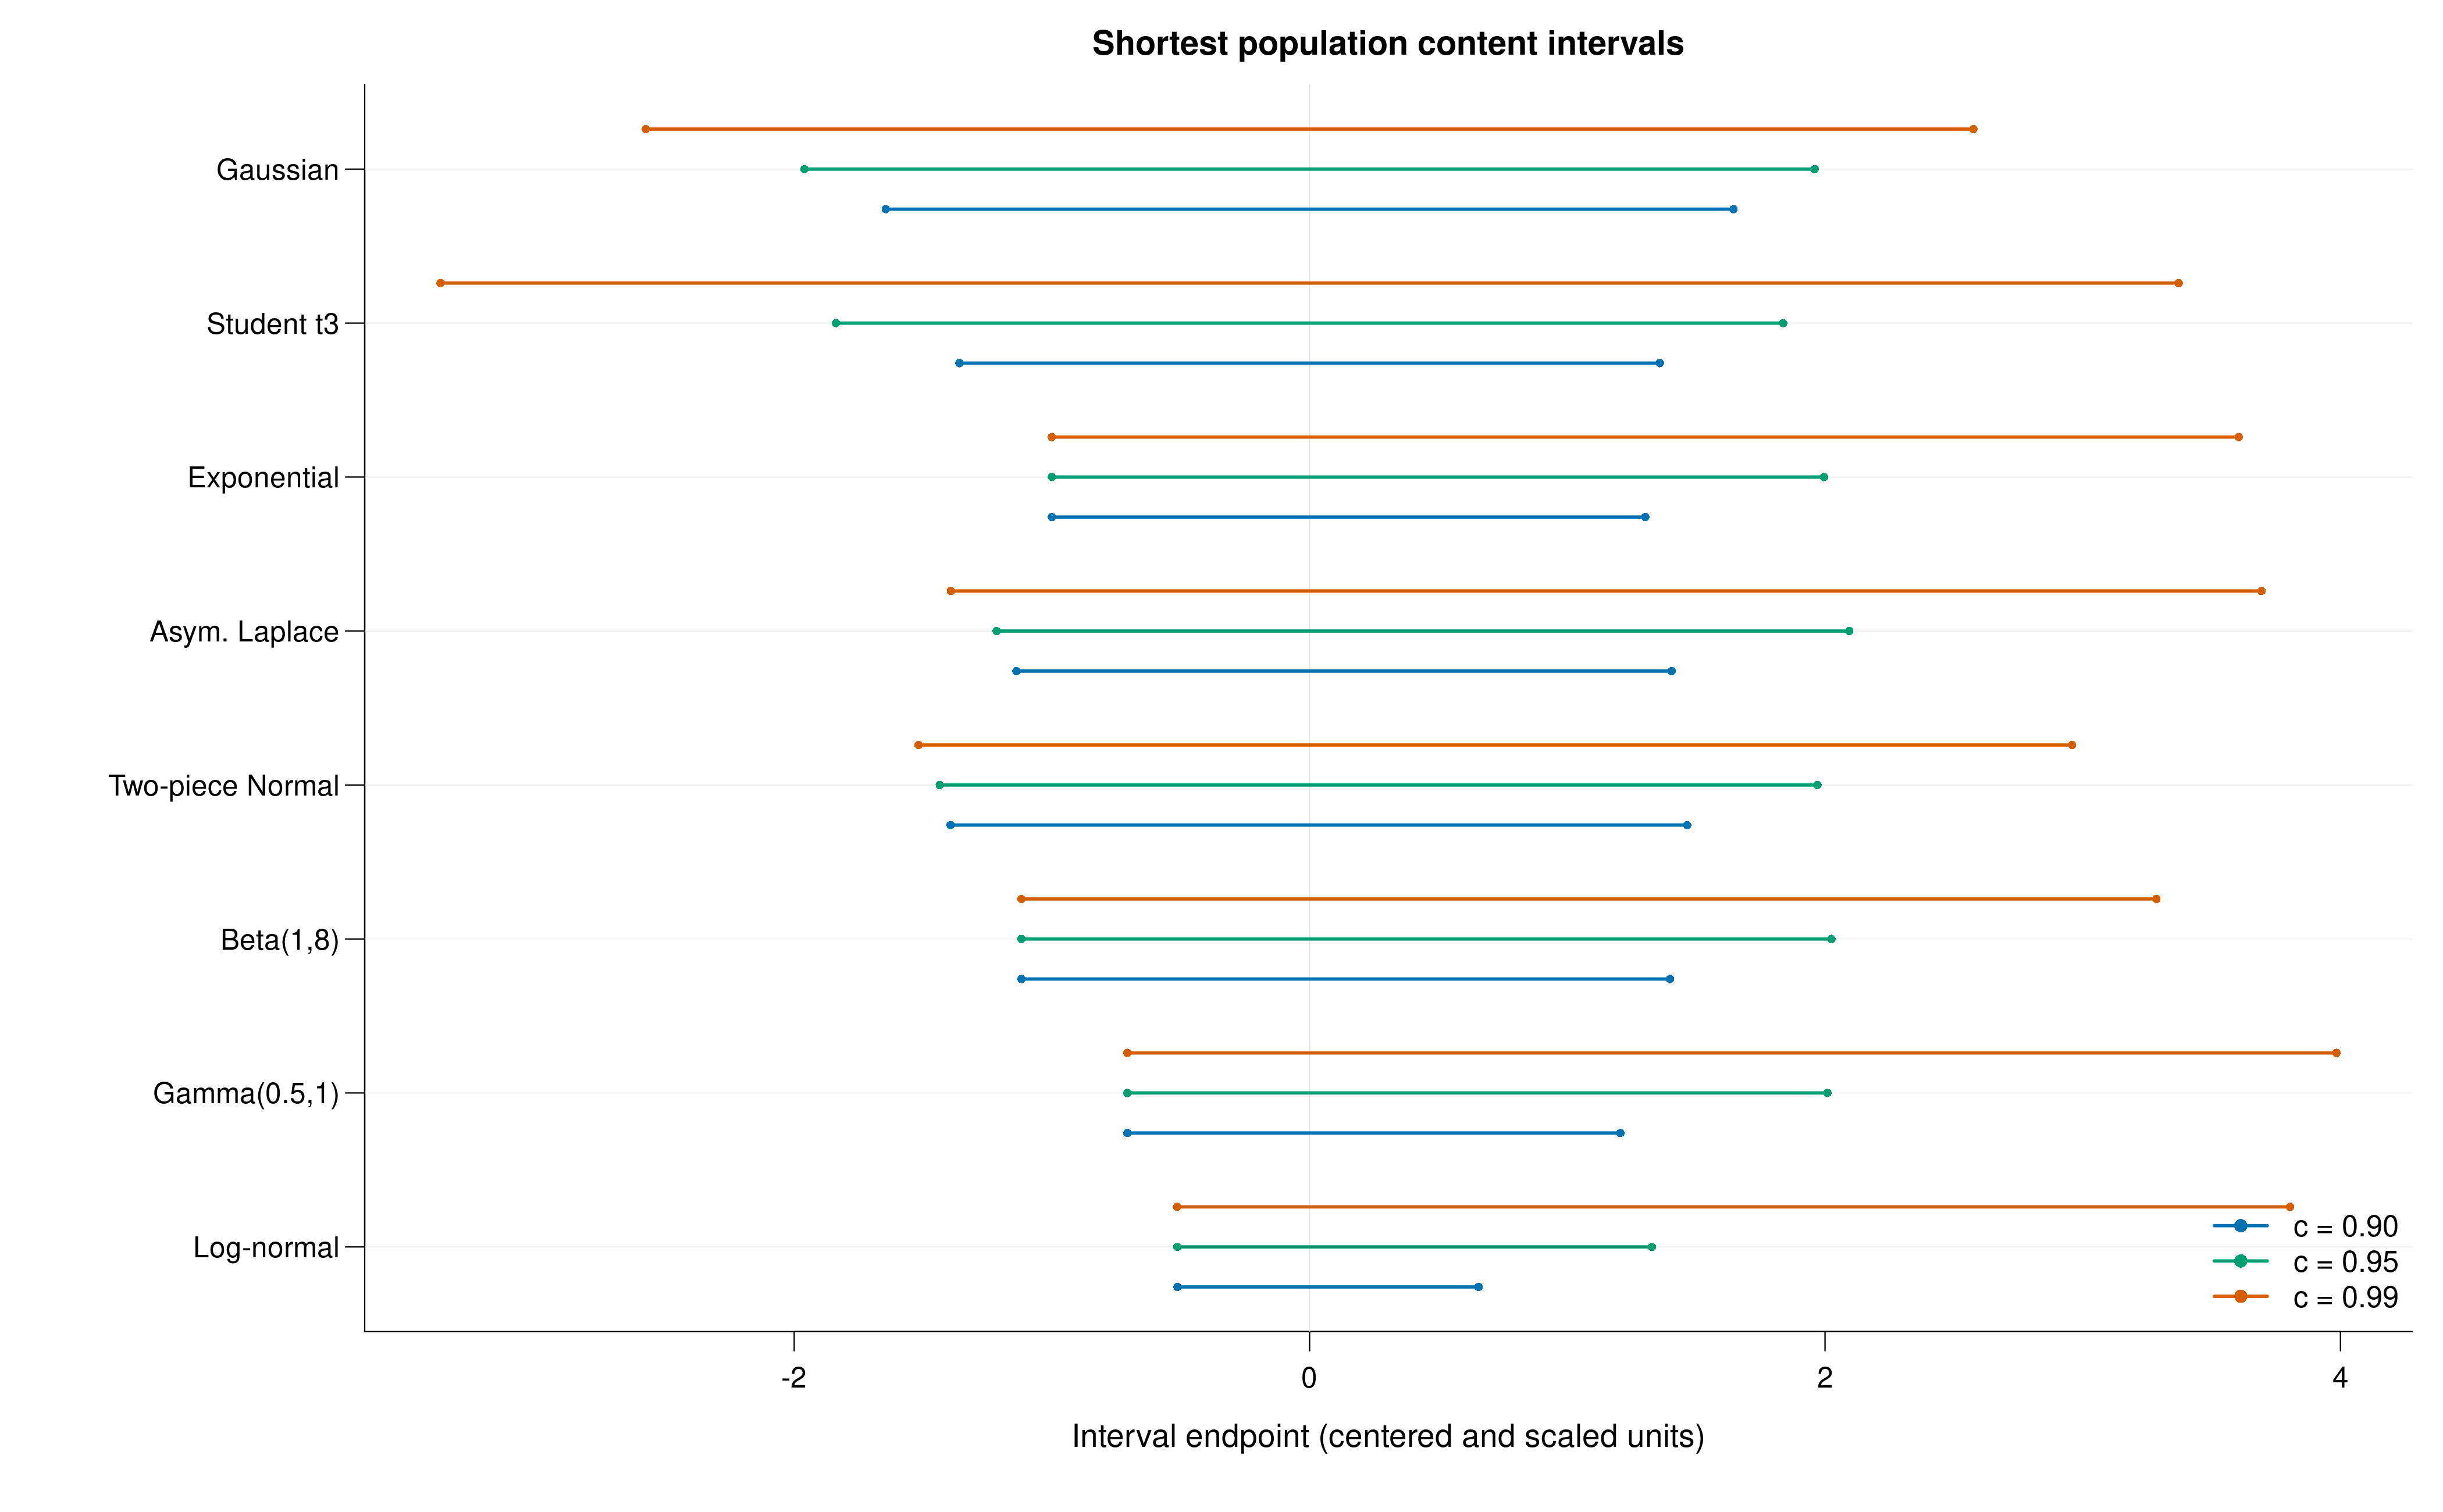
\includegraphics[width=\textwidth]{figures/ch05-mti/generated/figS03_tolerance_population_shortest_intervals.png}
\caption{\textbf{Population shortest-content intervals for the simulation
distributions.} Horizontal intervals show the shortest population content-\(c\)
intervals for the centered and scaled simulation laws. The figure supplies the
width benchmarks used to interpret the empirical width ranges in the main
article.}
\label{rqr:fig:supp-tolerance-population-shortest}
\end{figure}

These results are empirical repeated-sampling evidence for the selected
profile rule; the finite-sample distribution-free guarantee comes from the TCSP
scan calibration.

\begingroup
\scriptsize
\setlength{\tabcolsep}{3pt}
\begin{longtable}{@{}>{\raggedright\arraybackslash}p{0.16\textwidth}>{\centering\arraybackslash}p{0.12\textwidth}>{\centering\arraybackslash}p{0.17\textwidth}>{\centering\arraybackslash}p{0.16\textwidth}>{\centering\arraybackslash}p{0.12\textwidth}>{\centering\arraybackslash}p{0.19\textwidth}@{}}
\caption{\textbf{Selected adaptive MTI-ECM calibration rule.} The direct-DP content-probability check is fixed by a separate calibration run within each sample-size/content cell before the independent validation summaries are computed. Validation attainment is reported as the range across the eight simulation distributions.}\label{rqr:tab:supp-mti-ecm-policy}\\
\toprule
Cell & DP content level & Calibration lower probability & Validation range (\%) & Cells below 95\% & Width 95\% span
\\
\midrule
\endfirsthead
\toprule
Cell & DP content level & Calibration lower probability & Validation range (\%) & Cells below 95\% & Width 95\% span
\\
\midrule
\endhead
\(n=50,c=0.90\) & 0.995 & 0.966 & 95.8--97.8 & 0 & 1.53--13.76 \\
\(n=100,c=0.90\) & 0.995 & 0.986 & 98.5--99.7 & 0 & 1.5--5.75 \\
\(n=100,c=0.95\) & 0.995 & 0.962 & 95.1--97.5 & 0 & 2.28--17.68 \\
\(n=500,c=0.90\) & 0.995 & 0.983 & 97.3--99.7 & 0 & 1.25--3.86 \\
\(n=500,c=0.95\) & 0.995 & 0.983 & 97.0--99.2 & 0 & 1.99--5.45 \\
\(n=500,c=0.99\) & 0.995 & 0.954 & 95.2--97.4 & 0 & 4.54--28.5 \\
\(n=1000,c=0.90\) & 0.995 & 0.985 & 97.7--99.5 & 0 & 1.24--3.67 \\
\(n=1000,c=0.95\) & 0.995 & 0.987 & 96.7--99.9 & 0 & 1.96--4.73 \\
\(n=1000,c=0.99\) & 0.996 & 0.984 & 97.9--99.4 & 0 & 4.62--13.31 \\
\bottomrule
\end{longtable}
\endgroup


The TCSP calibration chooses the retained count \(k\) before seeing the
replicated samples. Table~\ref{rqr:tab:supp-tcsp-scan-calibration} records the
retained counts, retained fractions, content buffers, and lower confidence
bounds used in the simulation design. Adaptive Clopper--Pearson calibration
selects the retained count for each feasible sample-size/content cell before
any distribution-specific replications are evaluated. When \(k=n\), TCSP is forced to
use the full sample range and therefore coincides with Wilks as a reported
interval. This occurs for \((n,c)=(50,0.90),(100,0.95)\), and
\((500,0.99)\).

\begin{table}[H]
\centering
\caption{\textbf{TCSP scan calibration for the simulation design.} The retained
count \(k\) is selected by adaptive Clopper--Pearson Monte Carlo scan
calibration. The content buffer is \(k/n-c\).}
\label{rqr:tab:supp-tcsp-scan-calibration}
\TableStyle
\begin{tabular}{@{}rrrrrr@{}}
\toprule
\(n\) & \(c\) & Retained count \(k\) & \(k/n\) & Buffer \(k/n-c\) & Lower confidence bound\\
\midrule
50 & 0.90 & 50 & 1.000 & 0.100 & 0.966 \\
100 & 0.90 & 98 & 0.980 & 0.080 & 0.979 \\
100 & 0.95 & 100 & 1.000 & 0.050 & 0.963 \\
500 & 0.90 & 467 & 0.934 & 0.034 & 0.950 \\
500 & 0.95 & 487 & 0.974 & 0.024 & 0.951 \\
500 & 0.99 & 500 & 1.000 & 0.010 & 0.960 \\
1000 & 0.90 & 925 & 0.925 & 0.025 & 0.960 \\
1000 & 0.95 & 968 & 0.968 & 0.018 & 0.958 \\
1000 & 0.99 & 998 & 0.998 & 0.008 & 0.975 \\
\bottomrule
\end{tabular}

\end{table}

Small-sample feasibility is governed by the full-range two-sided order-statistic
coverage probability
\[
  \Pr\{Y_{(1)}\le Y_{\mathrm{new}}\le Y_{(n)}
       \text{ for at least content } c\}
  =
  1-n(1-c)c^{n-1}-c^n .
\]
The smallest \(n\) satisfying this inequality depends on both content and
tolerance confidence. Table~\ref{rqr:tab:supp-full-range-thresholds} lists the
thresholds used to design the simulation study.

\begin{table}[H]
\centering
\caption{\textbf{Full-range feasibility thresholds.} Entries are the smallest
sample sizes for which the full-sample interval \([Y_{(1)},Y_{(n)}]\) reaches
the stated two-sided distribution-free content/confidence pair.}
\label{rqr:tab:supp-full-range-thresholds}
\TableStyle
\begin{tabular}{@{}lrrr@{}}
\toprule
Tolerance confidence & \(c=0.90\) & \(c=0.95\) & \(c=0.99\)\\
\midrule
\(0.90\) & 38 & 77 & 388\\
\(0.95\) & 46 & 93 & 473\\
\bottomrule
\end{tabular}
\end{table}

This distinction matters for interpreting the small sample sizes in
\citet{rqr-PourmohamadRichardsonSanso2026CalibratedBNP}. The values
\((38,77,388)\) are appropriate at \(90\%\) tolerance confidence. A
\(95\%\)-confidence design needs the larger thresholds \((46,93,473)\). The
simulation design therefore lists the feasible cells explicitly instead of
forming a Cartesian product of sample sizes and contents. This prevents the
comparison from treating structural infeasibility as a method failure.
The Young--Mathew comparator is evaluated through the \texttt{tolerance}
package's \texttt{nptol.int(..., method = "YM")} function. The completed
run used \texttt{tolerance} version 3.0.0, and the package version is included
in the method reproducibility record.

\section{Pharmaceutical Batch Application}
\label{rqr:sec:pharma-application}

We next apply the four reported procedures to the pharmaceutical-manufacturing
data of \citet{rqr-ZagarMihelic2022PharmaManufacturing}, using the public
\texttt{Laboratory.csv} file \citep{rqr-ZagarMihelic2021LaboratoryCsv}. The
application is descriptive: the simulation study above provides the controlled
evidence about tolerance performance. Here the goal is to show how the
prespecified interval rules place endpoints on observed batch-level data.

One observation corresponds to one manufacturing batch. We restrict attention
to product code 23, which gives 187 batches with a common recorded strength and
batch size. This restriction reduces heterogeneity before applying two-sided
interval procedures.

The main response is the reported film-coated-tablet tensile-strength measure.
The public file does not give product-specific acceptance criteria or a
resolved physical unit for this derived field, so the fitted intervals are
interpreted as statistical summaries of historical batch-to-batch variation.
They are not regulatory specifications, release limits, or process-control
limits. A content-defined two-sided interval is a reasonable descriptive
summary for this example because unusually low and unusually high tablet
strength may both be relevant to handling and performance.

The application uses \(c=0.90\) and tolerance confidence \(0.95\). For each of
1000 paired splits, all methods are fitted to the same \(n=100\) training
batches and evaluated on the remaining 87 batches. TCSP uses the same
adaptive Clopper--Pearson scan convention as the simulation study; for this
cell the retained count is \(k=98\). MTI-ECM uses the frozen selected policy
from the simulation calibration, with no tuning on the pharmaceutical data.
Young--Mathew and Wilks are evaluated with the same endpoint conventions as in
Section~\ref{rqr:sec:evaluation}. The split exercise is not used to choose or tune
a method. Held-out empirical content is interpreted only as a finite-data
stability check on the withheld batches, with the nominal tolerance-confidence
claim anchored in the simulation-calibrated procedure.

\begin{table}[!htbp]
\centering
\caption{\textbf{Pharmaceutical tensile-strength application.} Intervals are
fit on 100 code-23 batches and evaluated on the 87 held-out batches over 1000
paired splits. Width and held-out content summaries report medians with
empirical 2.5\%--97.5\% ranges across splits. Omitted below/above gives the
median held-out percentage below the lower endpoint and above the upper
endpoint.}
\label{rqr:tab:pharma-application-primary}
\TableStyle
\begin{tabularx}{\textwidth}{@{}l>{\raggedright\arraybackslash}X>{\raggedright\arraybackslash}X>{\raggedright\arraybackslash}Xr@{}}
\toprule
Method & Median interval & Width median [95\% range] & Held-out content median [95\% range] & Omitted below/above\\
\midrule
TCSP & [1.101, 1.618] & 0.552 [0.462, 0.628] & 95.4 [88.5, 100.0] & 1.1 / 2.3 \\
MTI-ECM & [1.101, 1.618] & 0.552 [0.462, 0.628] & 95.4 [88.5, 100.0] & 1.1 / 2.3 \\
Young--Mathew & [1.137, 1.690] & 0.532 [0.452, 0.610] & 95.4 [88.5, 100.0] & 2.3 / 1.1 \\
Wilks & [1.040, 1.748] & 0.665 [0.535, 0.708] & 98.9 [93.1, 100.0] & 0.0 / 0.0 \\
\bottomrule
\end{tabularx}

\end{table}

\begin{figure}[!htbp]
\centering
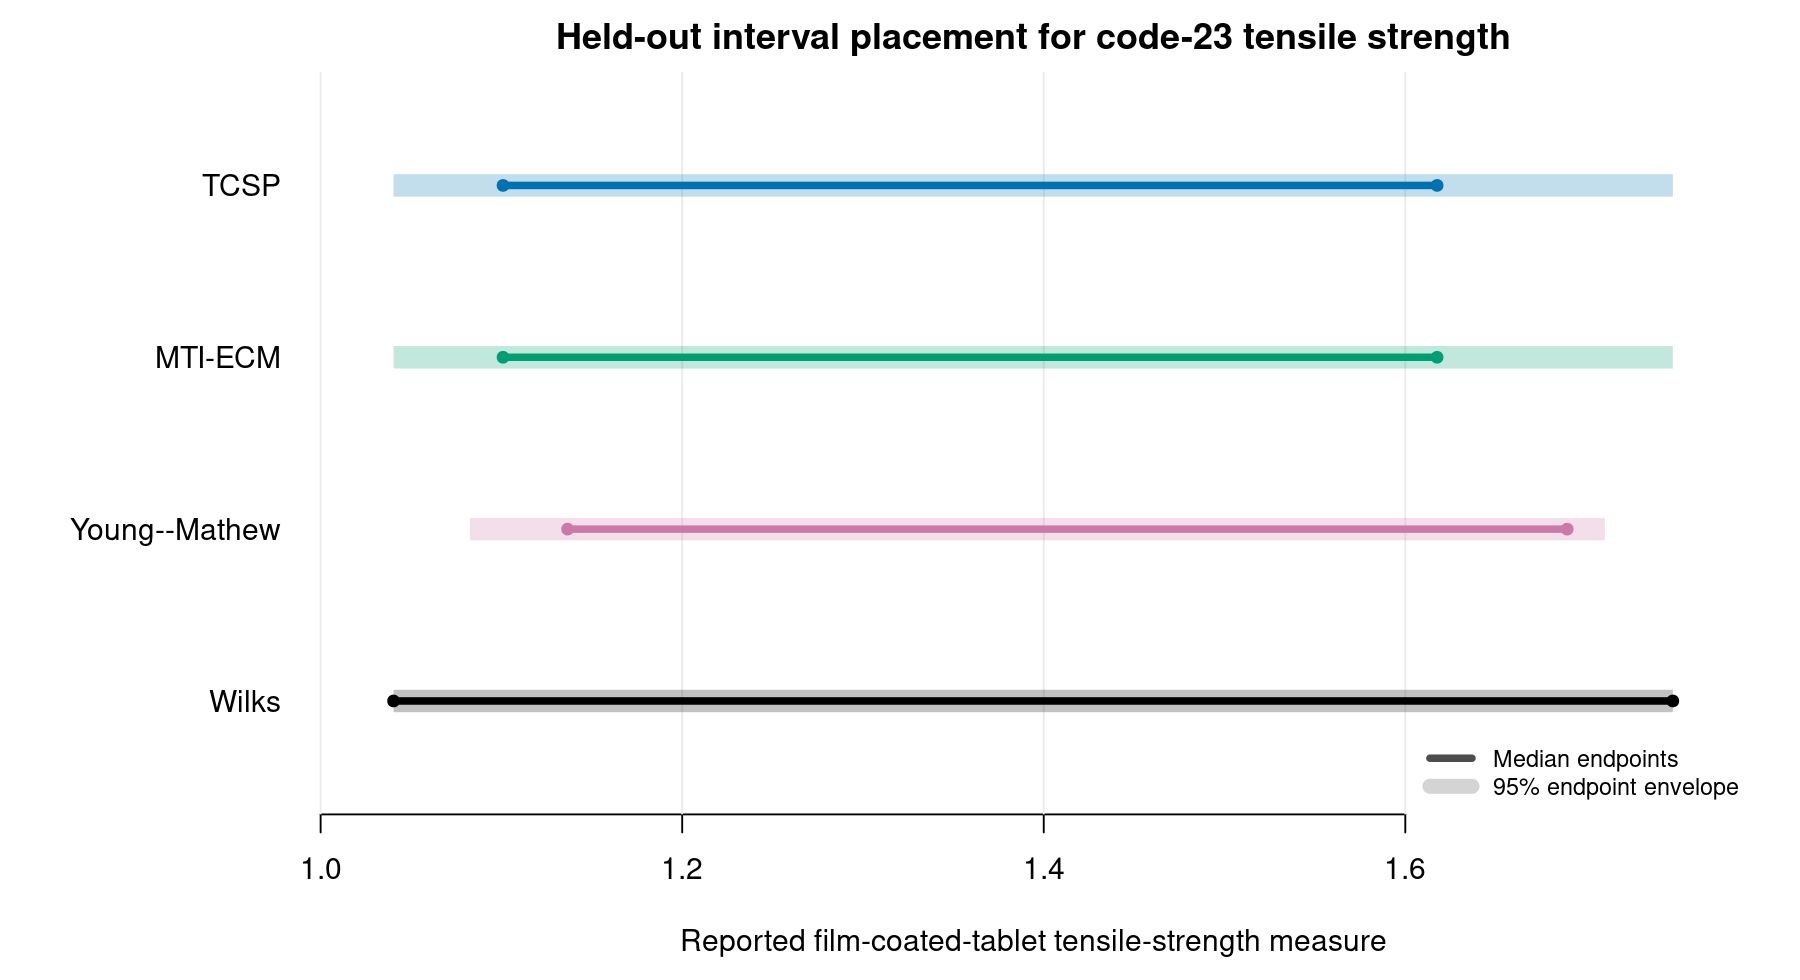
\includegraphics[width=\textwidth]{figures/ch05-mti/generated/fig06_pharma_application_tensile_intervals.png}
\caption{\textbf{Endpoint placement in the pharmaceutical application.} Thick
segments show median endpoints across paired splits; pale segments show the
empirical 95\% endpoint envelope. TCSP and the frozen MTI-ECM rule coincide to
the displayed precision for this response, Young--Mathew shifts the median
interval upward, and Wilks uses a wider range.}
\label{rqr:fig:pharma-application-primary}
\end{figure}

For the tensile-strength measure, TCSP and the frozen MTI-ECM rule produce the
same displayed median interval, \([1.101,1.618]\), with median width \(0.552\).
Young--Mathew is slightly shorter in median width but shifts the interval
upward and has the same median held-out content. Wilks has higher held-out
content because it uses the full sample range more often, but its median width
is larger. These patterns support the application's role as an interpretability
check, with method comparisons remaining anchored in the controlled simulation
study. The integrated material repeats the analysis for tablet-core weight relative
standard deviation, a strongly right-skewed response for which the two-sided
analysis is useful for studying placement but an upper tolerance limit would be
more natural for a direct quality-control decision.

\section{Pharmaceutical Application Details}
\label{rqr:sec:supp-pharma-application}

The pharmaceutical application uses the public manufacturing data described by
\citet{rqr-ZagarMihelic2022PharmaManufacturing}. The analysis file is
\texttt{Laboratory.csv}, version 1 on Figshare
\citep{rqr-ZagarMihelic2021LaboratoryCsv}. The downloaded file contains 1005
batches and 55 recorded fields. The analysis script verifies the byte count and
MD5 digest before restricting the analysis to product code 23. This restriction
leaves 187 batches with recorded strength \(20\)M and size 960000.
The analysis is descriptive and uses procedures fixed before examining these
responses. It illustrates endpoint placement on observed manufacturing batches;
the tolerance-confidence evidence in the paper comes from the controlled
simulation study.

\begin{table}[H]
\centering
\caption{\textbf{Application response diagnostics for product code 23.}
The tensile-strength measure is used in the main article. The weight-RSD
response is reported here because it is more strongly right-skewed but has a
mainly upper-adverse quality interpretation. Film-coated-tablet hardness is not
used because the recorded values have more ties on the observed scale.}
\label{rqr:tab:supp-pharma-response-diagnostics}
\TableStyle
\setlength{\tabcolsep}{2pt}\begin{tabular}{@{}llrrrrrr@{}}
\toprule
Role & Response & Batches & Distinct & Largest tie & Median & SD & Skewness\\
\midrule
Main & fct\_tensile & 187 & 82 & 11 & 1.341 & 0.124 & 0.44 \\
Supplement & tbl\_rsd\_weight & 187 & 83 & 6 & 1.030 & 0.467 & 3.00 \\
Excluded & fct\_av\_hardness & 187 & 32 & 17 & 70.560 & 6.459 & 0.48 \\
\bottomrule
\end{tabular}

\end{table}

For each of 1000 paired splits, all four methods use the same 100 training
batches and the same 87 held-out batches. TCSP uses the retained count
\(k=98\) from the adaptive scan calibration for \(n=100\), \(c=0.90\), and
tolerance confidence \(0.95\). MTI-ECM uses the frozen selected calibration
policy from the independent simulation validation, with direct
Dirichlet-process content-probability threshold \(0.995\). The fitted content
and tilt are selected by the prespecified MTI-ECM rule within each training
sample; the rule itself is not tuned on these pharmaceutical responses. The
held-out empirical summaries describe stability within the finite historical
data set, with repeated-sampling tolerance assessment left to the simulation
study.

\begin{table}[H]
\centering
\caption{\textbf{Additional weight-RSD application.} Intervals are fit on
100 code-23 batches and evaluated on the 87 held-out batches over 1000 paired
splits. Width and held-out content summaries report medians with empirical
2.5\%--97.5\% ranges across splits.}
\label{rqr:tab:supp-pharma-rsd}
\TableStyle
\begin{tabularx}{\textwidth}{@{}l>{\raggedright\arraybackslash}X>{\raggedright\arraybackslash}X>{\raggedright\arraybackslash}Xr@{}}
\toprule
Method & Median interval & Width median [95\% range] & Held-out content median [95\% range] & Omitted below/above\\
\midrule
TCSP & [0.600, 2.610] & 2.000 [1.527, 2.370] & 96.6 [89.7, 100.0] & 0.0 / 2.3 \\
MTI-ECM & [0.600, 2.610] & 2.000 [1.527, 2.370] & 96.6 [89.7, 100.0] & 0.0 / 2.3 \\
Young--Mathew & [0.700, 2.970] & 2.260 [1.572, 2.589] & 95.4 [87.4, 98.9] & 3.4 / 1.1 \\
Wilks & [0.600, 4.050] & 3.370 [1.818, 3.450] & 98.9 [93.1, 100.0] & 0.0 / 0.0 \\
\bottomrule
\end{tabularx}

\end{table}

\begin{figure}[H]
\centering
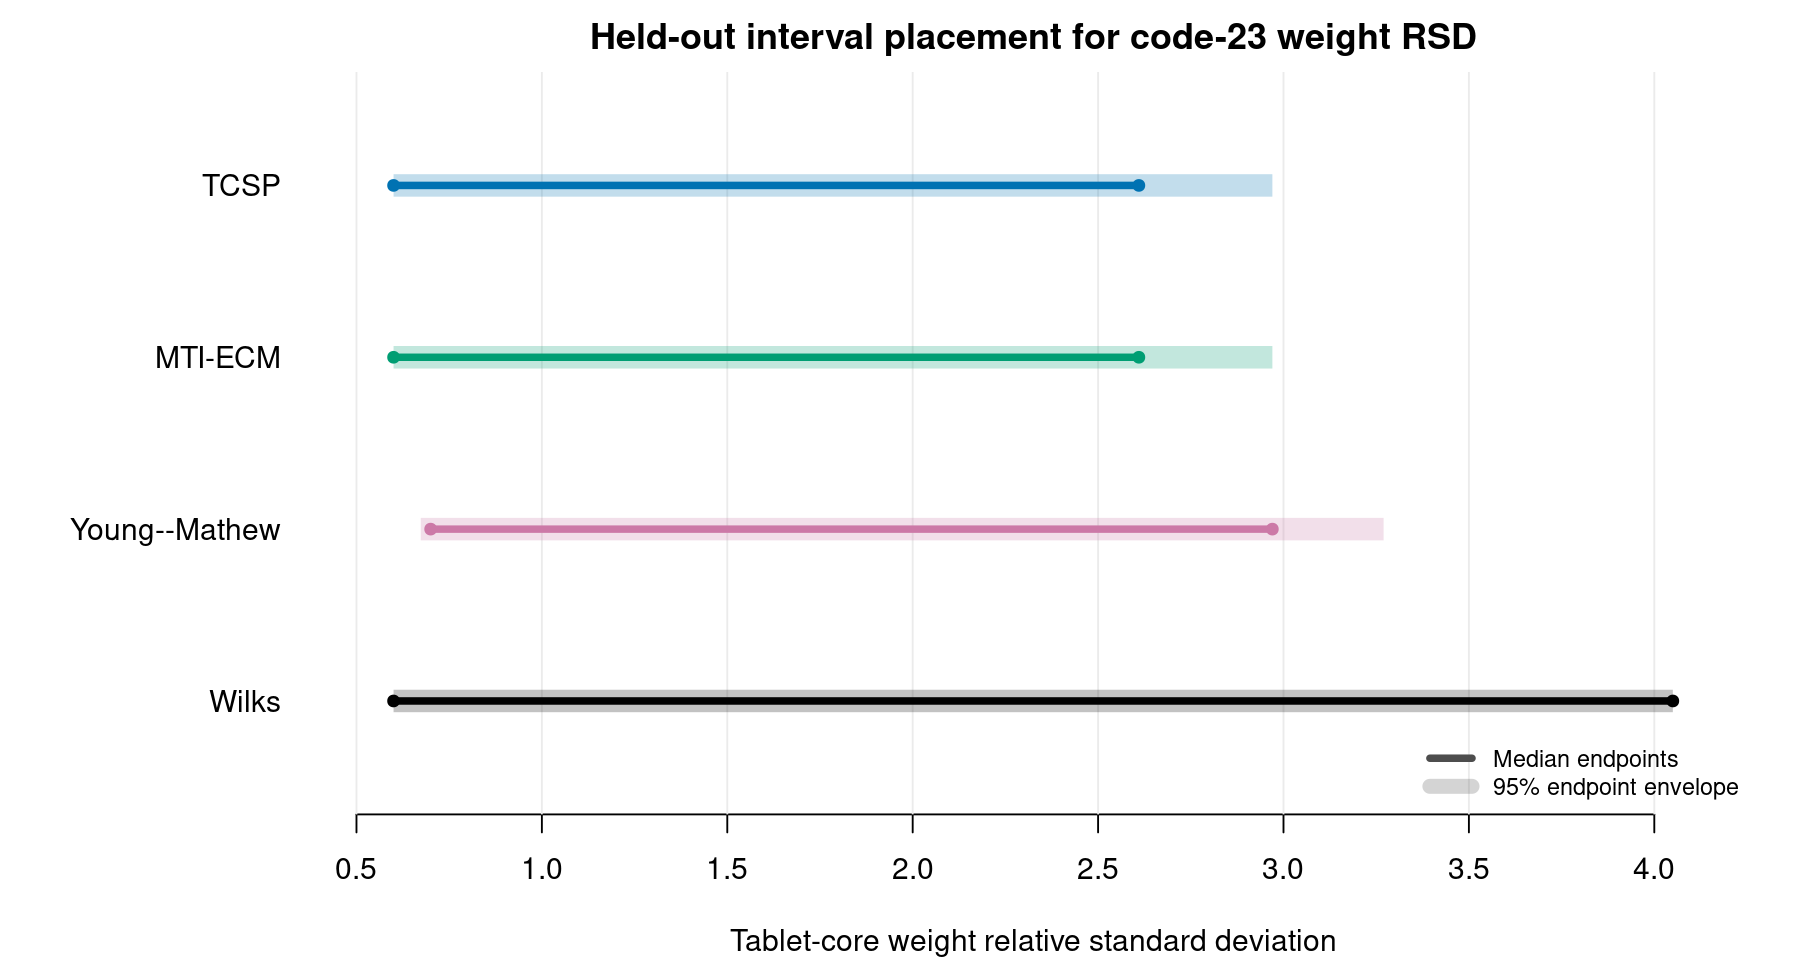
\includegraphics[width=\textwidth]{figures/ch05-mti/generated/figS04_pharma_application_rsd_intervals.png}
\caption{\textbf{Endpoint placement for tablet-core weight RSD.} Thick
segments show median endpoints across paired splits; pale segments show the
empirical 95\% endpoint envelope. The response is strongly right-skewed, so the
two-sided interval is interpreted as a placement analysis rather than as a
direct quality-control rule.}
\label{rqr:fig:supp-pharma-rsd}
\end{figure}

Held-out content was also summarized within production month, API batch, and
batch-order quartile whenever a held-out group contained at least three
observations. These checks are descriptive because the splits are drawn from a
finite historical data set rather than from a controlled independent
experiment. The summaries in Table~\ref{rqr:tab:supp-pharma-dependence} indicate
how much held-out content varies across recorded batch groupings.

\begin{table}[H]
\centering
\caption{\textbf{Held-out grouping sensitivity in the pharmaceutical
application.} Entries summarize, across paired splits, the within-split range
of empirical content across groups with at least three held-out batches.}
\label{rqr:tab:supp-pharma-dependence}
\TableStyle
\begin{tabularx}{\textwidth}{@{}lllrr@{}}
\toprule
Response & Grouping & Method & Median range & 97.5\% range\\
\midrule
Tensile strength & API batch & TCSP & 33.3 & 100.0 \\
Tensile strength & API batch & MTI-ECM & 33.3 & 100.0 \\
Tensile strength & API batch & Young--Mathew & 33.3 & 100.0 \\
Tensile strength & API batch & Wilks & 25.0 & 66.7 \\
Tensile strength & Batch-order quartile & TCSP & 8.0 & 21.1 \\
Tensile strength & Batch-order quartile & MTI-ECM & 8.0 & 21.1 \\
Tensile strength & Batch-order quartile & Young--Mathew & 8.7 & 26.5 \\
Tensile strength & Batch-order quartile & Wilks & 4.5 & 15.8 \\
Tensile strength & Production month & TCSP & 33.3 & 75.0 \\
Tensile strength & Production month & MTI-ECM & 33.3 & 75.0 \\
Tensile strength & Production month & Young--Mathew & 33.3 & 80.0 \\
Tensile strength & Production month & Wilks & 25.0 & 66.7 \\
Weight RSD & API batch & TCSP & 33.3 & 100.0 \\
Weight RSD & API batch & MTI-ECM & 33.3 & 100.0 \\
Weight RSD & API batch & Young--Mathew & 33.3 & 100.0 \\
Weight RSD & API batch & Wilks & 25.0 & 33.3 \\
Weight RSD & Batch-order quartile & TCSP & 8.7 & 27.2 \\
Weight RSD & Batch-order quartile & MTI-ECM & 8.7 & 27.2 \\
Weight RSD & Batch-order quartile & Young--Mathew & 10.4 & 27.3 \\
Weight RSD & Batch-order quartile & Wilks & 4.8 & 15.5 \\
Weight RSD & Production month & TCSP & 25.0 & 50.0 \\
Weight RSD & Production month & MTI-ECM & 25.0 & 50.0 \\
Weight RSD & Production month & Young--Mathew & 33.3 & 66.7 \\
Weight RSD & Production month & Wilks & 14.3 & 33.3 \\
\bottomrule
\end{tabularx}

\end{table}

\section{Reproducibility and Validation Limits}
\label{rqr:sec:supp-reproducibility}

The reproducibility materials separate mathematical statements, numerical
construction, and repeated-sampling evidence. The proofs above support the
population MPI and MTI identities, the fractional empirical score balance, and
the direct DP fixed-interval content law under their stated assumptions. The
TCSP retained counts are calibrated before the replicated samples are analyzed.
The MTI-ECM content-probability check and stability rule are selected in a separate
calibration run and then applied unchanged in the independent validation run.

The validation evidence is confined to iid continuous univariate samples from
the prespecified simulation distributions. It does not establish tolerance
validity for regression intervals, dynamic endpoint states, dependent samples,
or response-predictive distributions. Those extensions require their own
targets, assumptions, algorithms, diagnostics, and validation designs.

\section{Discussion}
\label{rqr:sec:discussion}

Probability content alone determines a class of interval placements. MPI selects
the mean-preserving member under the stated population conditions. MTI
generalizes MPI by making retained-mean balance a fixed coordinate:
\(\delta=0\) returns MPI, and admissible nonzero tilts specify other contiguous
content-\(c\) windows. Equal-tailed and shortest-contiguous intervals are
therefore distribution-specific members of the same placement family.

The tolerance contribution is a separate frequentist layer. A scan statistic
chooses an empirical retained count, after which the shortest closed
order-statistic window at that count is reported. This makes TCSP the primary
tolerance procedure and gives a class-specific minimum-width property within the
calibrated empirical scan class. The validation study shows that TCSP gives
reliable content attainment across the feasible design cells while avoiding much
of the width inflation of full-range Wilks intervals. The calibrated MTI-ECM
comparator links the empirical study to the MTI loss and can be shorter in many
cells, but its evidence is repeated-sampling validation of a selected rule
rather than a distribution-free finite-sample theorem.

The separation between target, computation, and tolerance guarantees is essential. MTI
identifies which fixed-content interval is being estimated. A generalized
posterior describes uncertainty for a fixed loss-defined target. A response
model, such as a direct Dirichlet-process posterior for \(F\), gives
model-based content probabilities. Tolerance confidence in TCSP comes from the
scan calibration. Moving a guarantee from one layer to another requires a
separate theorem or direct validation study.

The pharmaceutical application has a narrower role. It demonstrates how the
precalibrated procedures behave on historical batch data, while the
repeated-sampling tolerance evidence comes from the simulation design.

Several limitations remain. The TCSP statement is iid, continuous, and
univariate, and it uses the closed order-statistic convention stated in the
paper. Boundary tilts can lead to one-sided limits or inactive roots, and tilts
outside the admissible range do not define a finite unrestricted target.
Regression-family and dynamic tolerance calibration, selected-interval
asymptotics, exact scan recursion, and posterior-to-interval transfer remain open
problems. These topics are better treated in a companion development focused on
endpoint regression and dynamic computation, where the evidence standards differ
from the finite-sample tolerance procedure studied here.

\section{Regression and dynamic endpoint extensions}
\noindent
Mean-tilted intervals (MTI) provide a fixed-content family of interval targets
indexed by retained-mean balance. This paper develops generalized-Bayes
computation for using those targets in regression and time-varying endpoint
models after content and tilt have been specified. The update combines a prior
with an exponentiated residual-product check loss, yielding uncertainty
summaries for endpoint functions rather than a response-distribution model.

The pseudo-AL normal--exponential representation gives
generalized-inverse-Gaussian latent-scale updates and Gaussian conditional
updates for one root when the other is fixed. The same representation gives
deterministic ECM equations for generalized-posterior modes. We present ridge
endpoint regression, a conditionally Gaussian shrinkage construction for the
zero-tilt case, deterministic basis-expansion endpoint models, and dynamic linear
endpoint states updated by alternating forward-filtering backward-sampling
steps. These methods extend the MTI target from iid intervals to regression and
dynamic settings; tolerance guarantees and response prediction require
separate calibration or response models.

\subsection{Introduction}
\label{mti:sec:introduction}

Intervals with the same probability content can represent different statistical
targets. Equal-tailed, mean-preserving, and shortest-contiguous intervals share
content but differ in endpoint placement. The companion tolerance paper
develops this geometry and uses it to define scan-calibrated tolerance
procedures.
The present paper focuses on a different question: once a fixed-content target
has been specified, how can endpoint functions be estimated and summarized in
regression and time-varying settings?

The starting point is the residual-product criterion introduced by
\citet{rqr-PouplinEtAl2024RQR}. For ordered endpoints \(a<b\), the product
residual \((y-a)(y-b)\) is negative exactly when \(y\) lies inside the interval.
With a check loss applied to this scalar residual, the unrestricted population
score equations identify the mean-preserving interval (MPI). MTI generalizes
MPI by adding a fixed retained-mean tilt \(\delta\), so that different
admissible fixed-content windows are represented by different tilt values.

This paper treats MPI and MTI as loss-defined targets. For a fixed content
\(c\), tilt \(\delta\), and learning rate \(\omega_{\mathrm R}\), a
generalized posterior is obtained by updating a prior with
\(\exp\{-\omega_{\mathrm R}L_{c,\delta,n}\}\)
\citep{rqr-BissiriHolmesWalker2016GeneralBayes}. This update is useful for
regularization and uncertainty summaries for endpoint functions. Because the
update targets endpoints, posterior endpoint draws should be interpreted as
uncertainty summaries for the interval functional. Repeated-sampling tolerance
statements require a separate calibration layer.

The contributions are threefold. First, we formulate static endpoint regression
for MPI and fixed-tilt MTI, including the root-label symmetry and the
midpoint-gap summaries needed for interpretation. Second, we derive a
pseudo-asymmetric-Laplace augmentation that gives Gaussian conditional root
updates, generalized-inverse-Gaussian latent-scale updates, and a deterministic
ECM mode algorithm. Third, we show how the same fixed-target computation extends
to deterministic basis expansions and to dynamic linear endpoint states through
alternating root-specific smoothing updates.

The formal setting is deliberately bounded. Nonzero tilt is treated as fixed before
fitting or selected by an external rule. The conditionally Gaussian shrinkage
construction is stated for the MPI case unless an additional propriety argument
is supplied. Dynamic endpoint models describe time-varying interval-root
functionals under the chosen loss and prior; they do not inherit the iid
tolerance guarantee studied in the companion paper.

\subsection{Fixed-Content Targets and Generalized Bayes}
\label{mti:sec:targets}

Let \(Y\) have a continuous distribution with finite mean \(\mu\), and let
\(c\in(0,1)\) denote the desired interval content. For endpoints \(a<b\), define
\[
e(a,b;y)=(y-a)(y-b),
\qquad
\rho_c(r)=r\{c-\ind(r<0)\}.
\]
The MPI loss is
\[
\ell_c^{\mathrm{MPI}}(a,b;y)=\rho_c\{e(a,b;y)\}.
\]
At an unrestricted regular population stationary point, the score equations
give
\[
\Pr(a<Y<b)=c,
\qquad
\E(Y\mid a<Y<b)=\mu.
\]
Thus MPI selects the content-\(c\) interval whose retained mean equals the full
mean.

MTI replaces zero retained-mean balance by a fixed offset. In midpoint and
half-width coordinates \(a=m-h\), \(b=m+h\), the fixed-tilt loss can be written
\[
\ell_{c,\delta}(m,h;y)
=\rho_c\{(y-m)^2-h^2\}-2c\delta(y-m).
\]
At a regular unrestricted stationary point,
\[
\Pr(|Y-m|<h)=c,
\qquad
\E(Y\mid |Y-m|<h)=\mu+\delta .
\]
The tilt \(\delta\) is part of the target specification. Treating it as an
ordinary unknown inside the same posterior would average over distinct interval
targets.

For data \(D_n=\{(x_i,y_i):i=1,\ldots,n\}\), write the two raw root functions as
\(\eta_1(x;\theta_1)\) and \(\eta_2(x;\theta_2)\). Given fixed
\((c,\delta,\omega_{\mathrm R})\), the generalized posterior is
\begin{equation}
\pi(\theta_1,\theta_2\mid D_n)
\propto
\exp\{-\omega_{\mathrm R}L_{c,\delta,n}(\theta_1,\theta_2)\}
\pi_0(\theta_1,\theta_2).
\label{mti:eq:generalized-posterior}
\end{equation}
The learning rate controls the scale of the loss update. It is distinct from
the content \(c\), the tilt \(\delta\), and any response-distribution parameter.

\subsection{Static Endpoint Regression}
\label{mti:sec:static-regression}

In static linear endpoint regression, the raw roots are
\[
\eta_{1i}=x_i^\top\beta_1,\qquad
\eta_{2i}=x_i^\top\beta_2.
\]
The loss is symmetric in the two roots. Lower and upper endpoints are therefore
reported after sorting the fitted root values,
\[
L_i=\min(\eta_{1i},\eta_{2i}),\qquad
U_i=\max(\eta_{1i},\eta_{2i}),\qquad
W_i=U_i-L_i.
\]
This sorting is applied to endpoint functionals, not to individual regression
coefficients.

The midpoint-gap coordinates clarify which summaries are invariant to root
labels:
\[
\beta_m=\frac{\beta_1+\beta_2}{2},
\qquad
\beta_s=\frac{\beta_2-\beta_1}{2}.
\]
At a design row \(x\),
\[
M(x)=x^\top\beta_m,\qquad
S(x)=x^\top\beta_s,
\]
and
\[
L(x)=M(x)-|S(x)|,\qquad
U(x)=M(x)+|S(x)|,\qquad
W(x)=2|S(x)|.
\]
The vector \(\beta_m\) is the coefficient vector for the geometric midpoint.
The signed vector \(\beta_s\) is an orientation coordinate for the gap. A direct
lower-endpoint and upper-endpoint coefficient interpretation requires a design
region where one root remains below the other.

Ridge priors give a regularized default for fixed-dimensional endpoint regression.
Let
\[
\beta_j\sim\Normal(b_{0j},P_{0j}^{-1}),\qquad j=1,2,
\]
with proper precision matrices \(P_{0j}\). Proper Gaussian priors are also
useful for fixed nonzero tilt because the tilt term is linear in the root
parameters and the Gaussian prior has finite moment-generating functions in
finite dimensions.

\subsection{Pseudo-AL Computation}
\label{mti:sec:pseudo-al}

The product-residual check loss admits a normal-exponential representation
analogous to the asymmetric-Laplace construction used in Bayesian quantile
regression \citep{env-yu2001bayesian,qdesn-KozumiKobayashi2011Gibbs}. Let
\[
\sigma_{\mathrm R}=\omega_{\mathrm R}^{-1},\qquad
\xi_c=\frac{1-2c}{c(1-c)},\qquad
\phi_c=\frac{2}{c(1-c)}.
\]
For \(e_i=(y_i-\eta_{1i})(y_i-\eta_{2i})\),
\begin{align}
&\frac{c(1-c)}{\sigma_{\mathrm R}}
\exp\{-\rho_c(e_i)/\sigma_{\mathrm R}\}\notag\\
&\quad=
\int_0^\infty
\Normal(e_i\mid \xi_cv_i,\phi_c\sigma_{\mathrm R}v_i)
\Exp(v_i\mid\mathrm{rate}=1/\sigma_{\mathrm R})\,dv_i .
\label{mti:eq:pseudo-al}
\end{align}
This identity augments the generalized-posterior factor in
\eqref{mti:eq:generalized-posterior}. The resulting kernel is defined on product
residuals and should be interpreted as a loss factor for endpoints; a sampling
density for \(Y_i\) would require an additional response model.

The latent-scale full conditional is
\[
v_i\mid\cdot\sim
\GIG\left\{
\frac12,\
\frac{1}{2\sigma_{\mathrm R}c(1-c)},\
\frac{c(1-c)e_i^2}{2\sigma_{\mathrm R}}
\right\}.
\]
Conditional on \((v_i)\) and one root, the other root has a Gaussian update.
For example, holding \(\eta_2\) fixed, define
\[
\mat A_1=\diag(y_i-\eta_{2i})\mat X,\qquad
z_1=y\circ(y-\eta_2)-\xi_c v.
\]
With weight matrix
\[
\mat W_v=\diag\{(\phi_c\sigma_{\mathrm R}v_i)^{-1}\},
\]
the canonical parameters for \(\beta_1\) are
\[
\mat Q_1=P_{01}+\mat A_1^\top\mat W_v\mat A_1,
\qquad
h_1=P_{01}b_{01}+\mat A_1^\top\mat W_v z_1.
\]
The conditional update is
\[
\beta_1\mid\cdot\sim \Normal(\mat Q_1^{-1}h_1,\mat Q_1^{-1}).
\]
The update for \(\beta_2\) is obtained by exchanging root labels.

For fixed nonzero tilt, the conditional precision is unchanged and the
canonical vector receives the additive shift
\[
h_1^{\mathrm{MTI}}
=h_1+\omega_{\mathrm R}c\mat X^\top\delta ,
\]
with the same form for the second root. This is the main computational
convenience of the fixed-tilt construction.

The same augmentation yields an ECM mode calculation
\citep{rqr-DempsterLairdRubin1977EM,rqr-MengRubin1993ECM}. For \(e_i\ne0\),
\[
E(v_i^{-1}\mid\cdot)=\frac{1}{c(1-c)|e_i|}.
\]
Using these inverse-scale moments, the conditional maximization for each root
is a Gaussian ridge solve. The numerical implementation uses objective
backtracking and deterministic multi-start selection, because the joint
criterion is not globally quadratic in the two roots.

\subsection{Basis Expansions and Time-Varying Endpoints}
\label{mti:sec:extensions}

Deterministic basis expansions use the static regression equations with a
larger fixed design matrix. For example, a precomputed echo-state or deep
echo-state representation supplies a deterministic nonlinear basis
\(h_i\), after which the root functions are
\[
\eta_{1i}=h_i^\top\beta_1,\qquad
\eta_{2i}=h_i^\top\beta_2.
\]
The recurrent basis construction is part of the predictor representation. The
generalized posterior remains the fixed-target endpoint update in
\eqref{mti:eq:generalized-posterior}. The choices used to form the basis should be
stated as part of the validation design.

Time-varying endpoint models replace static coefficients by root-specific state
trajectories. A basic dynamic linear specification is
\[
\eta_{jt}=f_t^\top\theta_{jt},\qquad
\theta_{jt}=G_t\theta_{j,t-1}+\varepsilon_{jt},\qquad j=1,2,
\]
with Gaussian state innovations. The stacked prior over both root paths is
Gaussian. The product residual makes the joint augmented log density quartic in
the two paths together, but conditional on one complete root path the other path
has a linear Gaussian observation equation. Alternating root-specific
forward-filtering backward-sampling steps therefore gives a natural blocked
sampler for the specified fixed-target generalized posterior
\citep{env-goncalves}.

Discount factors and component scales affect the state prior and hence the
posterior target. Fixed discount templates can be treated as part of the model
specification. Adaptive discount or scale selection changes the inferential
target unless the selection rule is stated as part of a larger model or as a
separate sensitivity analysis.

\subsection{Uncertainty Calibration and Diagnostics}
\label{mti:sec:diagnostics}

The generalized posterior in \eqref{mti:eq:generalized-posterior} is centered at a
loss-defined target under standard local conditions, but its curvature
covariance need not equal the frequentist sandwich covariance. In fixed
dimension, open-faced-sandwich adjustment \citep{rqr-Shaby2014OpenFacedSandwich}
can be used as a post-processing calibration for differentiable coefficient or
endpoint summaries when consistent curvature and score-variance estimates are
available. This adjustment calibrates generalized-posterior uncertainty; it is
separate from any response-distribution model used for prediction.

For MCMC calculations, reporting should include the number of chains, warmup and
retained draws, convergence diagnostics, effective sample sizes, and any
root-label handling. For ECM calculations, reporting should include the
selected content and tilt, the final objective value, the number of iterations,
the stopping rule, and stability checks across starting values. For deterministic
basis-expansion and time-varying endpoint models, the basis construction, state prior,
and validation protocol should be stated before empirical comparisons are made.

Empirical evaluation must match the target. Endpoint regression can be assessed
through held-out MTI loss, empirical content, interval width, and recovery of
known endpoint functions in simulation. Tolerance validation requires a
content-confidence tolerance procedure, such as the TCSP construction in the companion
tolerance paper. Forecast evaluation requires a response-distribution model or a
clearly defined predictive interval rule.

\subsection{Discussion}
\label{mti:sec:discussion}

MTI provides a way to specify fixed-content interval placement through
retained-mean balance. The generalized-Bayes construction developed here turns a
chosen fixed-content target into regularized endpoint regression, deterministic
basis-expansion endpoint models, and time-varying endpoint models. The pseudo-AL augmentation
gives practical Gibbs and ECM computations while preserving the distinction
between a loss update and a response likelihood.

The main limitation is also the main organizing principle: content, endpoint
uncertainty, and tolerance confidence are different statistical statements.
Nonzero tilt should be fixed or selected by a separate rule before fitting.
Regression and time-varying endpoint models require their own validation before
claims about repeated-sampling tolerance behavior are made. This separation
keeps the computation extensible without overstating what the interval targets
imply.


\subsection{Integrated computational details}
\subsubsection{Notation and Targets}
\label{mti:sec:supp-targets}

For an observation \(y_i\) and raw roots \(\eta_{1i}\) and \(\eta_{2i}\),
define
\[
e_i=(y_i-\eta_{1i})(y_i-\eta_{2i}),\qquad
\rho_c(r)=r\{c-\ind(r<0)\}.
\]
The MPI loss is \(\rho_c(e_i)\). With fixed tilt \(\delta_i\), the MTI loss is
\[
\rho_c(e_i)-c\delta_i(\eta_{1i}+\eta_{2i}-2y_i).
\]
The cumulative loss over observed indices \(I_{\mathrm{obs}}\) is denoted by
\(L_{c,\delta}(\theta)\). The fixed-target generalized posterior is
\[
\pi(\theta\mid D)
\propto
\exp\{-\omega_{\mathrm R}L_{c,\delta}(\theta)\}\pi_0(\theta).
\]
The symbols \(c\), \(\delta\), and \(\omega_{\mathrm R}\) have different roles:
content, retained-mean tilt, and learning rate, respectively.

\subsubsection{Root Labels and Endpoint Summaries}
\label{mti:sec:supp-labels}

The product-residual loss is invariant to exchanging the two raw roots. With
exchangeable root priors, the unordered pair is identified but the labels
``root 1'' and ``root 2'' are not. Endpoint summaries are therefore computed
after sorting the roots at the evaluation points:
\[
L_i=\min(\eta_{1i},\eta_{2i}),\qquad
U_i=\max(\eta_{1i},\eta_{2i}),\qquad
W_i=U_i-L_i.
\]

For static linear roots, define
\[
\beta_m=\frac{\beta_1+\beta_2}{2},\qquad
\beta_s=\frac{\beta_2-\beta_1}{2}.
\]
Then \(M(x)=x^\top\beta_m\), \(S(x)=x^\top\beta_s\), and
\[
L(x)=M(x)-|S(x)|,\qquad
U(x)=M(x)+|S(x)|,\qquad
W(x)=2|S(x)|.
\]
The midpoint coefficient \(\beta_m\) is root-label invariant. The signed gap
coefficient \(\beta_s\) changes sign under a root swap. Lower- and
upper-endpoint coefficient summaries require a declared design region where the
two roots remain ordered.

\subsubsection{Pseudo-AL Augmentation}
\label{mti:sec:supp-pseudo-al}

Let
\[
\sigma_{\mathrm R}=\omega_{\mathrm R}^{-1},\qquad
\xi_c=\frac{1-2c}{c(1-c)},\qquad
\phi_c=\frac{2}{c(1-c)}.
\]
The single-observation loss factor satisfies
\begin{align}
&\frac{c(1-c)}{\sigma_{\mathrm R}}
\exp\{-\rho_c(e_i)/\sigma_{\mathrm R}\}\notag\\
&\quad=\int_0^\infty
\Normal(e_i\mid \xi_cv_i,\phi_c\sigma_{\mathrm R}v_i)
\Exp(v_i\mid\mathrm{rate}=1/\sigma_{\mathrm R})\,dv_i .
\end{align}
Thus
\[
v_i\mid\cdot\sim
\GIG\left\{
\frac12,\
\frac{1}{2\sigma_{\mathrm R}c(1-c)},\
\frac{c(1-c)e_i^2}{2\sigma_{\mathrm R}}
\right\}.
\]
The latent scales are part of the computational representation of a
loss-based update. They are not latent response variables.

\subsubsection{Gaussian Root Updates and Fixed Tilt}
\label{mti:sec:supp-static-updates}

Let \(\mat X_{\mathrm{obs}}\) be the observed design matrix and let
\(\mat W_v=\diag\{(\phi_c\sigma_{\mathrm R}v_i)^{-1}:i\in I_{\mathrm{obs}}\}\).
Conditional on the second root, define
\[
\mat A_1=\diag(\vect y_{\mathrm{obs}}-\vect\eta_{2,\mathrm{obs}})
\mat X_{\mathrm{obs}},
\qquad
\vect z_1=\vect y_{\mathrm{obs}}\circ
(\vect y_{\mathrm{obs}}-\vect\eta_{2,\mathrm{obs}})-\xi_c\vect v.
\]
For Gaussian prior canonical parameters \((\mat Q_{01},\vect h_{01})\),
\[
\mat Q_1=\mat Q_{01}+\mat A_1^\top\mat W_v\mat A_1,\qquad
\vect h_1=\vect h_{01}+\mat A_1^\top\mat W_v\vect z_1.
\]
Hence
\[
\beta_1\mid\cdot\sim
\Normal(\mat Q_1^{-1}\vect h_1,\mat Q_1^{-1}).
\]
The second root is updated by exchanging labels.

For fixed nonzero tilt, let \(\vect\delta_{\mathrm{obs}}\) be fixed over the
observed design. The precision matrix is unchanged, and the canonical vector is
shifted to
\[
\vect h_1^{\mathrm{MTI}}
=\vect h_1+
\omega_{\mathrm R}c\mat X_{\mathrm{obs}}^\top\vect\delta_{\mathrm{obs}},
\]
with the same shift for the second root. Proper Gaussian priors give a finite
normalizing constant in finite dimension because the tilt is linear in the
roots.

\subsubsection{ECM Mode Calculation}
\label{mti:sec:supp-ecm}

The ECM calculation maximizes the fixed generalized-posterior kernel. It uses
the exact inverse-scale moment
\[
\tau_i=E(v_i^{-1}\mid\cdot)=\frac{1}{c(1-c)|e_i|}
\]
away from \(e_i=0\), with a prespecified numerical floor near zero. Holding
\(\beta_2\) fixed, set
\[
\mat B_1=\diag(\vect y_{\mathrm{obs}}-\vect\eta_{2,\mathrm{obs}})
\mat X_{\mathrm{obs}},
\qquad
\vect r_1=\vect y_{\mathrm{obs}}^{\,2}
-\vect y_{\mathrm{obs}}\circ\vect\eta_{2,\mathrm{obs}}.
\]
With ridge prior precision \(\mat P_1\), the conditional maximization solves
\[
\left\{\mat P_1+
\frac{1}{\phi_c\sigma_{\mathrm R}}\mat B_1^\top\diag(\vect\tau)\mat B_1
\right\}\beta_1
=
\frac{1}{\phi_c\sigma_{\mathrm R}}
\mat B_1^\top\{\diag(\vect\tau)\vect r_1-\xi_c\vect 1\}
+\omega_{\mathrm R}c\mat X_{\mathrm{obs}}^\top\vect\delta_{\mathrm{obs}}.
\]
The second root uses the same equation with labels exchanged. A full ECM cycle
updates the latent-scale moments, solves the two conditional Gaussian systems,
and accepts the result only if the exact penalized objective decreases.

\subsubsection{Conditionally Gaussian Shrinkage}
\label{mti:sec:supp-shrinkage}

The zero-tilt MPI sampler can use a conditionally Gaussian regularized
horseshoe prior through the Nishimura--Suchard representation
\citep{qdesn-CarvalhoPolsonScott2010HS,qdesn-PiironenVehtari2017RHS,exd-nishimura2023shrunken}.
Conditional on the local, global, and slab-scale states, each root coefficient
block has a Gaussian prior precision and therefore fits directly into the
Gaussian update above. This construction is stated for MPI. Extending nonzero
tilt through random shrinkage scales requires its own propriety and diagnostic
checks.

\subsubsection{Deterministic Basis Expansions}
\label{mti:sec:supp-features}

Let \(\mat X_{\mathrm F}\) denote a deterministic basis matrix obtained before
the endpoint update is fitted. The static formulas apply with
\(\mat X_{\mathrm{obs}}\) replaced by the observed rows of
\(\mat X_{\mathrm F}\). Echo-state and deep echo-state basis functions
\citep{qdesn-Jaeger2001EchoState,qdesn-GallicchioMicheliPedrelli2018DeepESNDesign} are one
source of such a matrix. The recurrent representation is part of the design
construction; posterior uncertainty in the endpoint model is conditional on the
chosen basis unless the basis-generation mechanism is included in the
model.

\subsubsection{Dynamic Endpoint-State Updates}
\label{mti:sec:supp-dynamic}

A dynamic endpoint model replaces static coefficients by root-specific state
trajectories,
\[
\eta_{jt}=f_t^\top\theta_{jt},\qquad
\theta_{jt}=G_t\theta_{j,t-1}+\varepsilon_{jt},\qquad j=1,2.
\]
Gaussian initial and evolution distributions give a Gaussian prior over each
root path. Because the product residual contains both endpoint paths, the joint
augmented log density is quartic in the two paths. Conditional on one complete
path, however, the other path has a linear Gaussian observation equation.
Root-specific forward-filtering backward-sampling can therefore be alternated
within the specified fixed-target generalized posterior
\citep{env-goncalves}.

Discount factors and component scales are part of the state prior. Fixed values
or precomputed templates define a fixed target. Adaptive choices are best
reported as sensitivity analyses unless they are embedded in a fully specified
probability model.

\subsubsection{Diagnostics and Validation Limits}
\label{mti:sec:supp-diagnostics}

MCMC summaries should report multiple-chain convergence diagnostics, effective
sample sizes, Monte Carlo error, root-label handling, and endpoint functional
summaries. ECM summaries should report objective descent, iteration counts,
stopping criteria, final roots, fitted content, tilt, and sensitivity to
starting values. Basis-expansion analyses should report how the basis was
chosen. Dynamic analyses should report state-prior choices, smoothing
diagnostics, and whether discount or scale values were fixed in advance.

These diagnostics assess computation for a fixed endpoint target. They do not
establish tolerance validity or response-predictive calibration. Such claims
require a separate validation design aligned with the intended statistical
statement.
